%% ch19b：CuTe 官方白皮书中文导读（不编号，置于第四部分篇首）
%% 译自 Cris Cecka, "CuTe: Layout Representation and Algebra",
%% NVIDIA Research, arXiv:2603.02298v2（2026）。图、公式、代码均移植自
%% 官方公开 LaTeX 源 CuTeWhitepaper.tex，版权归原作者所有。
\begingroup
% --- 论文宏（仅本导读局部有效，出组即恢复全书定义）---
\def\CuTe{\textsc{CuTe}}
\def\R{\mathbb{R}}
\def\Q{\mathbb{Q}}
\def\Z{\mathbb{Z}}
\def\C{\mathbb{C}}
\def\N{\mathbb{N}}
\def\O{\mathcal{O}}
\def\D{\mathcal{D}}
\def\i{\imath}
\def\eps{\varepsilon}
\def\L{\mathcal{L}}
\def\E{\mathcal{E}}
\newcommand{\abs}[1]{\left| {#1} \right|}
\newcommand{\norm}[1]{\left\| {#1} \right\|}
\newcommand{\ceil}[1]{\left\lceil {#1} \right\rceil}
\newcommand{\floor}[1]{\left\lfloor {#1} \right\rfloor}
\def\v{\mathbf}
\def\bar#1{\overline{#1}}
\def\hat#1{\widehat{#1}}
\def\tilde#1{\widetilde{#1}}
\def\del{\nabla}
\def\d#1{\,\mathrm{d}{#1}}
\newcommand{\pluseq}{\mathrel{+}=}
\newcommand*\BitAnd{\mathbin{\&}}
\newcommand*\BitOr{\mathbin{|}}
\newcommand*\BitXor{\mathbin{\oplus}}
\newcommand*\BitNeg{\ensuremath{\mathord{\sim}}}
\newcommand*\ShiftLeft{\ll}
\newcommand*\ShiftRight{\gg}
\newcommand{\argmax}{\operatornamewithlimits{argmax}}
\newcommand{\sgn}{\operatorname{sgn}}
\newcommand{\diag}{\operatorname{diag}}
\def\epsilon{\varepsilon}
\newcommand{\pp}[2]{\frac{\partial #1}{\partial #2}}
\newcommand{\dd}[2]{\frac{\mathrm{d} #1}{\mathrm{d} #2}}
% 论文 paralist 的 compactitem 环境
\newenvironment{compactitem}{\begin{itemize}[itemsep=0pt,topsep=2pt]}{\end{itemize}}

% --- 导读内独立编号（不挂靠任何章号）---
\setcounter{section}{0}
\setcounter{subsection}{0}
\setcounter{subsubsection}{0}
\setcounter{figure}{0}
\setcounter{table}{0}
\setcounter{equation}{0}
\setcounter{theorem}{0}
\renewcommand{\thesection}{\arabic{section}}
\renewcommand{\thesubsection}{\arabic{section}.\arabic{subsection}}
\renewcommand{\thesubsubsection}{\arabic{section}.\arabic{subsection}.\arabic{subsubsection}}
\renewcommand{\thefigure}{W.\arabic{figure}}
\renewcommand{\thetable}{W.\arabic{table}}
\renewcommand{\theequation}{W.\arabic{equation}}
\renewcommand{\thetheorem}{W.\arabic{theorem}}
% 论文节标题映射：\section/\subsection/\subsubsection 正常编号并入目录
\def\wph#1{\section{#1}}
\def\wpsh#1{\subsection{#1}}
\def\wpssh#1{\subsubsection{#1}}

\chapter*{导读：CuTe 布局表示与代数\\（NVIDIA 官方白皮书中文译注）}
\addcontentsline{toc}{chapter}{导读：CuTe 布局表示与代数（白皮书中文译注）}
\markboth{导读：CuTe 布局表示与代数}{导读：CuTe 布局表示与代数}

\begin{center}
\small
原文：\textbf{Cris Cecka}，\emph{CuTe: Layout Representation and Algebra}，
NVIDIA Research，arXiv:2603.02298v2（2026）。\\[2pt]
本导读为该论文的完整中文翻译，全部插图（TikZ）、公式与代码均移植自论文官方
公开 \LaTeX{} 源 \texttt{CuTeWhitepaper.tex}，版权归原作者及 NVIDIA 所有，
本中译仅供学习使用。译文与全书第~20\textendash 26 章术语保持一致
（Product=乘积、Composition=复合、Coalesce=合并、Complement=补、
Divide=切分、Inverse=逆）。
\end{center}

\begin{quotation}\noindent\small
\textbf{摘要。}高性能计算与深度学习的现代体系结构越来越多地引入专用张量指令，
包括用于矩阵乘法的 Tensor Core 与面向多维数据的硬件优化拷贝操作。这些指令规定
了固定且往往十分复杂的数据布局，必须在整条执行流水线中被正确地传递，才能同时
保证正确性与最优性能。本文介绍 \CuTe{}——一套用于表示和操作张量的新颖数学规约。
\CuTe{} 提出两项关键创新：（1）层次化的布局表示，它是对传统扁平形状（flat
shape）与扁平步幅（flat stride）张量表示的直接推广，能够表达现代硬件指令所需
的复杂映射；（2）一套丰富的布局操作代数——包括拼接（concatenation）、合并
（coalescence）、复合（composition）、补（complementation）、切分（division）、
分块（tiling）与求逆（inversion）——支持复杂的布局操作、推导、验证与静态分析。
\CuTe{} 布局为管理 GPU kernel 中的数据布局与线程排布提供了统一框架，而布局代数
使得我们能够在编译期对布局性质进行强有力的推理，并简洁地表达通用张量变换。

在本文中我们将展示：与传统方法相比，\CuTe{} 的抽象显著助力软件开发，推动对体系
结构规定布局的编译期验证，便于实现可泛化到大量应用场景的算法原语，并能简洁地
表达现代专用张量指令所需的分块（tiling）与划分（partitioning）模式。

\CuTe{} 已成功部署于生产系统，是 NVIDIA CUTLASS 库以及包括 CuTe DSL 在内的一系
列相关工作的基础。我们同时给出数学基础与 Python 参考实现（PyCuTe），确立 \CuTe{}
作为面向以张量为中心的计算时代的、有原则的布局感知编程方法。
\end{quotation}

%% wp0 引言与动机（论文第 1 节）
\wph{引言与动机}

现代 GPU 越来越多地针对以张量（tensor）为中心的计算进行优化，其驱动力来自深度学习与科学计算的需求。NVIDIA 的 Volta 架构（NVIDIA，2017）引入了 Tensor Core，使硬件能够直接高效地完成小矩阵乘法。这一能力在 Turing（NVIDIA，2018）与 Ampere（NVIDIA，2021）中得到扩展，提供了在 GPU 内存层次结构中进行结构化矩阵搬运的专用指令。Hopper（NVIDIA，2023）与 Blackwell（NVIDIA，2025）架构进一步推进了这一范式，引入了在全球内存与共享内存之间高效传输 5 阶（rank）张量的拷贝指令，并进一步扩展了 Tensor Core 的能力。GPU 峰值性能很大程度上取决于这些面向张量的硬件特性能否被充分发挥，能高效表示与操作这些张量的高性能编程模型也就应运而生。

现有及新兴的硬件表现如何，很大程度上取决于多维数据在多个层次化内存空间与多个层次化并行级别中怎样被存储与访问。数据存储布局（layout）历来通过决定内存访问发生的方式与时机来影响性能；而随着硬件指令的规模越来越大，并为其输入输出规定了固定的布局，布局也开始决定正确性。这些布局必须沿整条执行流水线传递下去，才能保证硬件指令被正确调用，并保证内存访问模式得到优化。

在本工作中，我们呈现 \CuTe 的基础概念。\CuTe 是一项针对 \underline{CU}DA \underline{Te}nsors（即 \underline{C}ompute \underline{U}nified \underline{Te}nsors）的规约，旨在为编写峰值性能的线性代数库提供建构基石。\CuTe 的核心是两项关键创新：
\begin{compactitem}
\item {\em 一种新颖的张量布局表示}：\CuTe 的形状（shape）、布局与张量天然是层次化的，由更小的嵌套实例构造而成。这种层次结构提供了表示现代张量指令所需复杂映射的手段，同时仍是 {\tt BLAS}、{\tt torch.tensor}、{\tt numpy.ndarray} 与 MATLAB 等库中既有的扁平形状与扁平步幅（stride）表示的严格扩展。
\item {\em 一种定义在布局之上的新颖操作代数}：\CuTe 布局支持一组丰富的操作，包括拼接（concatenation）、合并（coalescence）、复合（composition）、补（complementation）、切分（division）、分块（tiling）与求逆（inversion），它们的结果都仍是新的 \CuTe 布局。这些操作支撑现代张量指令所需的复杂划分（partitioning）、操纵、验证与推导。
\end{compactitem}

\CuTe 的布局表示给通用算法一个直观的框架来管理线程与数据，布局代数则给高性能线性代数 kernel 的开发一条有表达力的路径，用来操纵布局、生成新布局。两者能带来：
\begin{compactitem}
\item 对复杂布局与划分的支持：\CuTe 便于表示应用特定数据模式所需的精细布局，以及专用张量指令所需的复杂划分模式。
\item 关注点分离：数据布局独立于算法逻辑进行声明，提升清晰性与模块化。
\item 静态分析与优化：精深的代数技术使我们能够依据体系结构约束对张量参数进行检查、重排与划分。
\end{compactitem}

\wpsh{相关工作}

\CuTe 的动机源于支持高效张量收缩开发的需求：张量收缩是众多科学计算与机器学习应用的核心。计算一般张量收缩的传统方法依赖矩阵化，即在逻辑上或显式地重组张量数据，以便通过一系列对基础线性代数子程序（BLAS）库的调用来完成计算。

%鉴于大多数张量收缩的理论计算与通信复杂度与矩阵乘法等价，张量收缩运算原则上能够以相似的效率扩展。

BLAS 为核心线性代数运算提供了高效且可移植的实现，并为广泛的体系结构提供了高度优化的版本（Blackford 等，2002）。在 BLAS 原语中，通用矩阵乘法（GEMM）例程无疑是全部科学计算与机器学习中被优化得最充分、使用最广泛的操作。

类 BLAS 库实例化软件（BLIS）框架（Van Zee 与 van de Geijn，2015）扩展了 GEMM，使其同时支持行模与列模中的非单位步幅，从而在不借助显式内存拷贝的情况下解决了处理不规则内存布局的部分挑战。BLAS 的跨步批量（strided-batched）GEMM 扩展进一步推广了该原语，使其能够应用于更多张量收缩（Shi 等，2016）。在对矩阵布局做更进一步的抽象时，启发 \CuTe 的思路是：在张量记号中使用多重索引，使任意张量收缩都能变换为规范化的 batched-GEMM 原语。

许多现有库都依赖张量，而它们几乎全都基于扁平形状与扁平步幅表示。在 Python 中，这包括 {\tt numpy.ndarray} 与 {\tt torch.tensor}：

\noindent
\begin{minipage}[t]{0.48\textwidth}
\begin{python}
>>> import numpy
>>> a = numpy.ndarray([3,7,5])
>>> a.dtype
dtype('float64')
>>> a.shape
(3, 7, 5)
>>> a.strides
(280, 40, 8)
\end{python}
\end{minipage}
\hfill
\begin{minipage}[t]{0.48\textwidth}
\begin{python}
>>> import torch
>>> a = torch.empty(3,7,5)
>>> a.dtype
torch.float32
>>> a.shape
torch.Size([3, 7, 5])
>>> a.stride()
(35, 5, 1)
\end{python}
\end{minipage}

\noindent 在 C++ 中，则是 {\tt std::mdspan}：

\noindent
\begin{cpp}
std::mdspan a = std::mdspan(data, 3, 7, 5);
a.extent(0);  // 3
a.extent(1);  // 7
a.extent(2);  // 5
a.stride(0);  // 35
a.stride(1);  // 5
a.stride(2);  // 1
\end{cpp}

\noindent \CuTe 支持这些表示，并对其做严格扩展：推广到层次化的形状与步幅，以表示更复杂的布局、非整数步幅以及非整数的布局陪域。

对稠密张量表示的独立推广还包括 HeLayers（Aharoni 等，2023）、ThunderKittens（Spector 等，2024），以及 OpenAI 的 Triton 编译器（Tillet 等，2019）中所使用的 Linear Layouts（Zhou 等，2025）方法。ThunderKittens 为寄存器内存、共享内存、行主序/列主序块、由行主序/列主序子块组成的行主序/列主序块，以及为 warp 与线程规定的访问模式实现了种类繁多的定制类型。这些类型的编写考虑了体系结构布局需求与内存层次，但其表示范围局限于既有的类型与模式。Linear Layouts 基于 $\mathbb{F}_2$ 线性代数，为张量布局提供了更一般的表示，也为布局分析与生成开辟了途径。但 Linear Layouts 对 $\mathbb{F}_2$ 的严格依赖使其中一些算子难以被人工检视，并将该工作限制在 2 的幂形状与步幅上，这对许多应用来说是不可接受的。

另一些启发了本工作部分内容的布局分析方法同样依赖 $\mathbb{F}_2$ 线性代数，例如 Edelman 等（1994）、Cormen（1993）与 Bouverot-Dupuis 及 Sheeran（2023）的工作。这些工作给出了分析与算法生成的出发点，但受限于其撰写时的应用语境。

由于 CUTLASS v3（NVIDIA，2023）中 \CuTe 的 C++ 实现是开源的并附有部分文档，它已在分析 \CuTe 布局与 \CuTe 代数操作的独立工作中被引用和使用。Bhaskaracharya 等（2025）在整数集关系（ISL）的语境下分析了 \CuTe 与 Linear Layouts（Zhou 等，2025），但略去了能将 Linear Layouts 表示为 \CuTe 布局的步幅抽象。LEGO（Tavakkoli 等，2025）在代码生成器中使用受限形式的 \CuTe 布局与原始形式的 \CuTe 复合来生成复杂索引。Carlisle 等（2026）则在范畴论的语境下分析了 \CuTe 布局及作用于其上的若干操作。
在本文中，我们打算对 \CuTe 概念及其应用给出更明确、更形式化的论述，并提供 \CuTe 的一个 Python 参考实现。
纯 Python 的参考实现 PyCuTe（NVIDIA，2026）可在 \url{https://github.com/NVlabs/CuTe} 获取，它与本文的定义与后置条件一一对应；它不同于面向 CUDA kernel JIT 编译的 CuTe DSL（NVIDIA，2025），也不同于 CUTLASS 中的 C++ CuTe 头文件。

\CuTe 的设计与概念已在若干应用中落地。例如，Graphene 张量编译器（Hagedorn 等，2023）用 \CuTe 表示张量运算；Stream-K 算法（Osama 等，2023）的实现用了 \CuTe 的 C++ 实现，NVIDIA CUTLASS v3 库（Kerr 等，2017）的开发也以它为核心。大型语言模型最先进的实现中也一直有它，FlashAttention 及其一代代演进（Dao 等，2022、Dao，2023、Shah 等，2024）就是例子，深度学习前沿的研究与应用处处用得上 \CuTe。一批相关编译器项目同样建在 \CuTe 之上，包括 CuTe DSL（NVIDIA，2025）：一种面向线性代数应用、基于 Python、动态编译 CUDA 软件的 DSL。

\wpsh{规范化循环与循环变换}
\label{sec:loops}

循环索引的显式计算是高性能线性代数 kernel 开发中的常见挑战。这些计算很难被程序员一次写对，维护起来更是难上加难。与其将数据访问信息与算法逻辑耦合在一起，我们更愿意用矩阵/向量坐标（coordinate）清晰地书写算法逻辑，而将数据访问模式抽象到数据布局之中。

为便于说明，我们首先定义本工作所发展的技术能够处理的循环嵌套类别。具体而言，我们把{\em 标准循环形式}（standard loop form）定义为具有单个索引、从零开始、以常量为界、且每次迭代递增 1 的循环。

例如，考虑如下循环：
\begin{cpp}
for (int m = 2; m <= 50; m += 3)
  A[m] = e(m);
\end{cpp}
该循环将 {\tt A[2]}、{\tt A[5]}、{\tt A[8]}、$\ldots$ 设为纯表达式 {\tt e(m)} 的结果。它可以变换为如下的规范化循环（canonical loop）：
\begin{cpp}
for (int i = 0; i < 17; ++i)
  (A + 2)[3*i] = g(i);
\end{cpp}
这里，指针偏移了一个循环不变常量，循环步幅被归一化为 1，下界变换为零，上界紧致且不含端点，纯表达式变换为 {\tt g(i) = e(3*i+2)}。现在，把上例理解为遍历一个逻辑上的 17 元素向量是很自然的：逻辑坐标以 3 为步幅，对基地址 {\tt A + 2} 处的数据进行索引。该程序可用如下数据表示：
\begin{verbatim}
Accessor: A + 2
   Shape: 17
  Stride: 3
\end{verbatim}
嵌套循环可以类似地处理。考虑如下的二维循环嵌套：
\begin{cpp}
for (int n = 3; n < 43; n += 2)
  for (int m = 4; m <= 22; m += 5)
    A[p*m + q*n] = e(m,n);
\end{cpp}
它可以变换为规范化循环形式：
\begin{cpp}
for (int j = 0; j < 20; ++j)
  for (int i = 0; i < 4; ++i)
    (A + 4*p + 3*q)[5*p*i + 2*q*j] = g(i,j);
\end{cpp}
有了规范化循环嵌套，很自然地可以把变换后的循环理解为遍历一个逻辑上的 $4 {\times} 20$ 矩阵：逻辑行坐标 $i$ 以 $5p$ 为步幅，逻辑列坐标 $j$ 以 $2q$ 为步幅，对基地址 {\tt A + 4*p + 3*q} 处的数据进行索引。这可以用如下数据表示：
\begin{verbatim}
Accessor: A + 4p + 3q
   Shape: ( 4, 20)
  Stride: (5p, 2q)
\end{verbatim}
一个关键观察是，$4 {\times} 20$ 矩阵也可以被解释为一个具有非均匀、半仿射步幅的 80 元素向量，用等价的规范化循环形式表达即为：
\begin{cpp}
for (int k = 0; k < 80; ++k)
  (A + 4*p + 3*q)[5*p*(k%4) + 2*q*(k/4)] = f(k);
\end{cpp}
其中 {\tt \%} 是取模运算，{\tt /} 是整数向下取整除法。这一变换是 2 维坐标 \verb|(i,j)| 与 1 维坐标 \verb|k| 之间的余字典序（colexicographical）双射 \verb|(i,j) = (k%4,k/4)|。
该双射与先前表示的形状等价，并可由其直接推导而来。因此，该形状表示既可以接受 2 维坐标，也可以接受 1 维坐标，为数据索引提供了一个灵活且与阶无关的框架。

规范化循环形式还为可证正确的循环变换提供了指导，这类变换经常出现在面向张量计算的优化编译器中。考虑最一般的规范化循环嵌套：
\begin{cpp}
for (int in = 0; in < Nn; ++in)
  ...
    for (int i1 = 0; i1 < N1; ++i1)
      for (int i0 = 0; i0 < N0; ++i0)
        A[d0*i0 + d1*i1 + ... + dn*in] = e(i0,i1,...,in);
\end{cpp}
其中 $(N_0, N_1, \ldots, N_n)$ 是计算的“形状”，$(d_0, d_1, \ldots, d_n)$ 是访问模式的“步幅”，
\begin{verbatim}
Accessor: A
   Shape: (N0,N1,...,Nn)
  Stride: (d0,d1,...,dn)
\end{verbatim}
由于 $\text{形状}:\text{步幅}$ 信息与循环嵌套本身之间存在一一对应，我们不必问“如何对循环施加变换——切分、转置、拼接、置换、截断、向量化等”，而是可以转而问：“$\text{形状}:\text{步幅}$ 表示的合法变换方式有哪些，又有哪些算子能提供这些变换？”事实上，若 $\v{L} = \text{形状}:\text{步幅}$ 表示数据访问与循环嵌套，那么存在哪些函数 $P$，使得
\begin{align*}
\v{L}' = P(\v{L}) = \v{L} \circ P
\end{align*}
构成从 $\v{L} = \text{形状}:\text{步幅}$ 到新循环嵌套 $\v{L}' = \text{形状}':\text{步幅}'$（可能具有新的形状与步幅）的一个有意义的变换？这些变换 $P$ 本质上是对循环嵌套的{\em 重写}，若定义得当，它们自身可以可复合、可求逆，并为命令式循环提供类似函数式编程的控制。结合上文讨论的 1 维坐标与 N 维坐标之间的双射，本文将证明：这些变换的一种非常有效的表示是 $P = \v{P} = \text{形状}^*:\text{步幅}^*$，正是我们用来表示数据访问与循环嵌套自身的同一类对象。

\wpsh{张量与折叠}

为了进一步阐述除 1 维坐标之外还能以 N 维坐标索引的形状这一动机，我们推广 Shi 等（2016）中将张量收缩映射到规范化类 BLAS 原语的观察。

在本工作中，张量用粗体字母表示，索引用小写字母表示，索引的界用对应的大写字母表示。张量的阶指它所拥有的维度（也称为模（mode））的数量。例如：
\begin{compactitem}
\item 标量 $\alpha$ 是 0 阶张量。
\item 向量 $\mathbf{a}_i$ 是 1 阶张量，其中 $0 \leq i < I$。
\item 矩阵 $\mathbf{A}_{mn}$ 是 2 阶张量，其中 $0 \leq m < M$ 且 $0 \leq n < N$。
\item 三路数组 $\mathbf{A}_{mnp}$ 是 3 阶张量，其中 $0 \leq m < M$、$0 \leq n < N$ 且 $0 \leq p < P$。
\end{compactitem}
对仅在等式单侧出现的重复索引隐含求和（爱因斯坦记号），因此张量收缩的一个实例是
\begin{align}
\v{C}_{stqp} = \v{A}_{stupr} \, \v{B}_{qtru},
\label{eqn:contraction}
\end{align}
它表示一个 5 阶张量与一个 4 阶张量收缩生成一个 4 阶张量。这类收缩在 {\tt numpy.einsum} 与 {\tt torch.einsum} 等接口中有紧凑的表达。

上面的张量收缩可以重写为
\begin{align*}
\v{C}_{(sp)(q)(t)} = \v{A}_{(sp)(ur)(t)} \, \v{B}_{(q)(ur)(t)},
\end{align*}
其中原张量收缩的各模被归为四类：
\begin{compactitem}
\item 行模（row modes）$\hat{m}$：出现在 $\v{A}$ 与 $\v{C}$ 中，而不出现在 $\v{B}$ 中。
\item 列模 $\hat{n}$：出现在 $\v{B}$ 与 $\v{C}$ 中，而不出现在 $\v{A}$ 中。
\item 归约模 $\hat{k}$：出现在 $\v{A}$ 与 $\v{B}$ 中，而不出现在 $\v{C}$ 中。
\item 批模 $\hat{\ell}$：出现在 $\v{A}$、$\v{B}$ 与 $\v{C}$ 中。
\end{compactitem}
这被称为张量{\em 折叠}（folding）。折叠一个张量并不需要任何显式拷贝，可以只是数据视图的变更。

作为张量折叠的一个显式例子，考虑图~\ref{fig:folding} 第一行所示的 8 元素 $2 {\times} 2 {\times} 2$ 张量。扁平表示为张量的每个模保存一个形状与一个步幅，用以索引物理数据。这种扁平表示与 C++ 的 {\tt std::mdspan}、PyTorch 的 {\tt torch.tensor}、NumPy 的 {\tt numpy.ndarray} 以及许多其它类似库所采用的表示完全相同。如第二行所示，通过将第三个模折叠进第一个模，该 $2 {\times} 2 {\times} 2$ 张量可以折叠成 $4 {\times} 2$ 矩阵。其结果可用形状为 $(4,2)$、步幅为 $(2,1)$ 的扁平表示。原则上，通过将第三个模折叠进第二个模，该 $2 {\times} 2 {\times} 2$ 张量也可以折叠成 $2 {\times} 4$ 矩阵。然而其结果不再具有扁平表示：不存在能表示第二个模的步幅的整数。

\begin{figure}[ht]
\centering
\scalebox{0.6}{
\begin{tikzpicture}[x={(0cm,-1cm)},y={(1cm,0cm)},every node/.style={minimum size=1cm, outer sep=0pt}]
\node[fill={rgb,255:red,175;green,175;blue,255}] at (0,0) {\Large a\strut};
\node[fill={rgb,255:red,175;green,175;blue,255}] at (0,1) {\Large b\strut};
\node[fill={rgb,255:red,175;green,255;blue,175}] at (0,2) {\Large c\strut};
\node[fill={rgb,255:red,175;green,255;blue,175}] at (0,3) {\Large d\strut};
\node[fill={rgb,255:red,255;green,255;blue,175}] at (0,4) {\Large e\strut};
\node[fill={rgb,255:red,255;green,255;blue,175}] at (0,5) {\Large f\strut};
\node[fill={rgb,255:red,255;green,175;blue,175}] at (0,6) {\Large g\strut};
\node[fill={rgb,255:red,255;green,175;blue,175}] at (0,7) {\Large h\strut};
\draw[color=black,thick,shift={(-0.5,-0.5)}] (0,0) grid (1,8);
\node at (-1,0) {\Large{\texttt{0}}};
\node at (-1,1) {\Large{\texttt{1}}};
\node at (-1,2) {\Large{\texttt{2}}};
\node at (-1,3) {\Large{\texttt{3}}};
\node at (-1,4) {\Large{\texttt{4}}};
\node at (-1,5) {\Large{\texttt{5}}};
\node at (-1,6) {\Large{\texttt{6}}};
\node at (-1,7) {\Large{\texttt{7}}};
\node at (1,3.5) {\Large 物理数据};
\end{tikzpicture}
}\\
\vspace{1em}
\begin{tabular}{|c|c|c|c|}
视图描述 & 视图图示 & 扁平表示 & \CuTe 表示 \\
\hline\hline
\shortstack{张量，$2 {\times} 2 {\times} 2$ \\ 3 阶} &
\scalebox{0.4}{
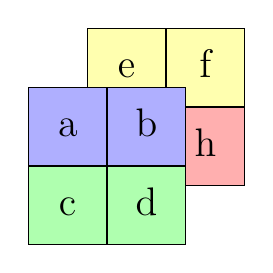
\begin{tikzpicture}[x={(0cm,-1cm)},y={(1cm,0cm)},every node/.style={minimum size=1cm, outer sep=0pt},baseline=(current bounding box.center)]
\node[draw=black, fill={rgb,255:red,255;green,255;blue,175}] at (0,0) {\Large e\strut};
\node[draw=black, fill={rgb,255:red,255;green,255;blue,175}] at (0,1) {\Large f\strut};
\node[draw=black, fill={rgb,255:red,255;green,175;blue,175}] at (1,0) {\Large g\strut};
\node[draw=black, fill={rgb,255:red,255;green,175;blue,175}] at (1,1) {\Large h\strut};
\node[draw=black, fill={rgb,255:red,175;green,175;blue,255}] at (0.75,-0.75) {\Large a\strut};
\node[draw=black, fill={rgb,255:red,175;green,175;blue,255}] at (0.75,0.25) {\Large b\strut};
\node[draw=black, fill={rgb,255:red,175;green,255;blue,175}] at (1.75,-0.75) {\Large c\strut};
\node[draw=black, fill={rgb,255:red,175;green,255;blue,175}] at (1.75,0.25) {\Large d\strut};
\end{tikzpicture}
} &
\shortstack{形状：$(2,2,2)$\\ 步幅：$(2,1,4)$} &
\shortstack{形状：$(2,2,2)$\\ 步幅：$(2,1,4)$} \\
\hline
\shortstack{矩阵，$4 {\times} 2$\\ 将模 2 折叠进模 0} &
\scalebox{0.4}{
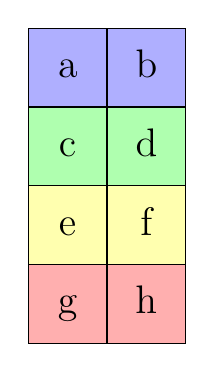
\begin{tikzpicture}[x={(0cm,-1cm)},y={(1cm,0cm)},every node/.style={minimum size=1cm, outer sep=0pt},baseline=(current bounding box.center)]
\node[draw=black, fill={rgb,255:red,175;green,175;blue,255}] at (0,0) {\Large a\strut};
\node[draw=black, fill={rgb,255:red,175;green,175;blue,255}] at (0,1) {\Large b\strut};
\node[draw=black, fill={rgb,255:red,175;green,255;blue,175}] at (1,0) {\Large c\strut};
\node[draw=black, fill={rgb,255:red,175;green,255;blue,175}] at (1,1) {\Large d\strut};
\node[draw=black, fill={rgb,255:red,255;green,255;blue,175}] at (2,0) {\Large e\strut};
\node[draw=black, fill={rgb,255:red,255;green,255;blue,175}] at (2,1) {\Large f\strut};
\node[draw=black, fill={rgb,255:red,255;green,175;blue,175}] at (3,0) {\Large g\strut};
\node[draw=black, fill={rgb,255:red,255;green,175;blue,175}] at (3,1) {\Large h\strut};
\end{tikzpicture}
} &
\shortstack{形状：$(4,2)$\\ 步幅：$(2,1)$} &
\shortstack{形状：$((2,2),2)$\\ 步幅：$((2,4),1)$} \\
\hline
\shortstack{矩阵，$2 {\times} 4$\\ 将模 2 折叠进模 1} &
\scalebox{0.4}{
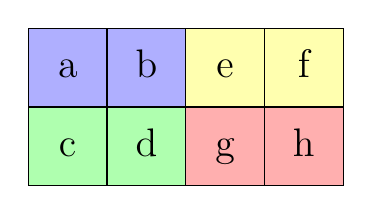
\begin{tikzpicture}[x={(0cm,-1cm)},y={(1cm,0cm)},every node/.style={minimum size=1cm, outer sep=0pt},baseline=(current bounding box.center)]
\node[draw=black, fill={rgb,255:red,175;green,175;blue,255}] at (0,0) {\Large a\strut};
\node[draw=black, fill={rgb,255:red,175;green,175;blue,255}] at (0,1) {\Large b\strut};
\node[draw=black, fill={rgb,255:red,175;green,255;blue,175}] at (1,0) {\Large c\strut};
\node[draw=black, fill={rgb,255:red,175;green,255;blue,175}] at (1,1) {\Large d\strut};
\node[draw=black, fill={rgb,255:red,255;green,255;blue,175}] at (0,2) {\Large e\strut};
\node[draw=black, fill={rgb,255:red,255;green,255;blue,175}] at (0,3) {\Large f\strut};
\node[draw=black, fill={rgb,255:red,255;green,175;blue,175}] at (1,2) {\Large g\strut};
\node[draw=black, fill={rgb,255:red,255;green,175;blue,175}] at (1,3) {\Large h\strut};
\end{tikzpicture}
} &
\shortstack{形状：$(2,4)$\\ 步幅：$(2,\text{\color{red}$\times$})$} &
\shortstack{形状：$(2,(2,2))$\\ 步幅：$(2,(1,4))$} \\
\hline
\end{tabular}
\caption{将一个 8 元素的物理数组视为 3 阶张量，并折叠为两个矩阵。}
\label{fig:folding}
\end{figure}

折叠后矩阵的 \CuTe 表示见最后一列，它强调张量折叠实际上只是把模分组。对 $4 {\times} 2$ 矩阵而言，扁平表示称为 \CuTe 表示的{\em 合并}版本；而对 $2 {\times} 4$ 矩阵，这样的扁平表示并不存在。

这种一般化的张量折叠形式使所有张量收缩都能写成单一的规范收缩形式：
\begin{align}
\mathbf{C}_{\hat{m}\hat{n}\hat{\ell}} = \mathbf{A}_{\hat{m}\hat{k}\hat{\ell}} \, \mathbf{B}_{\hat{n}\hat{k}\hat{\ell}}.
\end{align}
其中每个模可以是单个模，也可以是一组模，我们称之为{\em 多模}（multi-mode）。援引第~\ref{sec:loops} 节的规范化循环：无论 $\hat{m}$ 的形状是 $M$ 还是 $(M_0,M_1)$，我们都可以用 1 维坐标 $m$ 对其循环。于是，任何张量收缩都可以折叠为规范化的 {\tt batched-GEMM}，并用由四重嵌套循环组成的朴素参考实现求值：
\begin{cpp}
for (int l = 0; l < L; ++l)
  for (int m = 0; m < M; ++m)
    for (int n = 0; n < N; ++n)
      for (int k = 0; k < K; ++k)
        C(m,n,l) += A(m,k,l) * B(n,k,l);
\end{cpp}
只要巧妙地构造折叠布局，这个简单的 {\tt batched-GEMM} 实现便可用于求值范围广泛、相互兼容的张量收缩，包括任意矩阵乘法（{\tt GEMM}）、张量收缩（{\tt GETT}）与卷积（{\tt CONV}）。通用 {\tt GEMM} 及其应用的细节见第~\ref{sec:gemm} 节。

随后，优化便可专注于循环重排、分块、向量化这些常见手段，做法都是变换循环嵌套的顺序与阶。这些变换往往可以用布局表示为算法坐标空间上的置换。这些变换布局与数据布局进行函数式复合，生成新的循环嵌套，并保证与原始问题一致。布局复合及其在通用划分中的应用细节见第~\ref{sec:composition} 节。

%% wp1 布局表示：元组/形状/步幅（论文第 2 节前半）

\wph{布局表示（Layout Representation）}

\CuTe 布局（layout）是一类功能多样的对象，能够表示范围广泛的数据排列与线程排列，在抽象物理地址、将迭代顺序与存储顺序相分离等方面极具实用价值。在本节中，我们定义形状（shape）、布局与张量（tensor）的 \CuTe 表示，并说明它们与坐标（coordinate）如何相互作用。\CuTe 布局使得泛型算法只需单一实现，便可应用于任何可折叠为该算法规范形式（canonical form）的复杂数据布局。此类算法及其应用广度的示例见第~\ref{sec:algorithms}~节。

\wpsh{元组与层次元组（Tuple 与 HTuple）}

{\tt Tuple}（元组）与 {\tt HTuple}（层次元组）概念是贯穿本工作的基础数据结构。

\begin{definition}
$\texttt{Tuple}(\mathcal{T})$ 是从集合 $\mathcal{T}$ 中选取元素构成的有限有序列表。对于 $X = (X_0,X_1,\ldots,X_{n-1}) \in \texttt{Tuple}(\mathcal{X})$，我们定义如下运算：
\begin{compactitem}
\item {\bf 阶（rank）：}rank($X$)。即元组长度 $n$。
\item {\bf 访问（access）：}$X_i$。即 \texttt{Tuple} $X$ 的第 \texttt{i} 个元素，其中 $0 \leq i < \text{rank}(X)$。
\end{compactitem}
\end{definition}

\noindent $\texttt{Tuple}(\mathcal{T})$ 是元素的扁平（flat）集合，而 $\texttt{HTuple}(\mathcal{T})$ 则是“由 $\mathcal{T}$ 组成的层次元组”。

\begin{definition}
$\texttt{HTuple}(\mathcal{T})$ 或者是集合 $\mathcal{T}$ 中的一个元素，或者是一个 $\texttt{Tuple}(\texttt{HTuple}(\mathcal{T}))$。对于 $X \in \texttt{HTuple}(\mathcal{X})$，我们定义如下运算：
\begin{compactitem}
\item {\bf 阶（rank）：}rank($X$)。若 $X \in \texttt{Tuple}$，则为元组长度，否则为 1。
\item {\bf 访问（access）：}$X_i$。即 \texttt{HTuple} $X$ 的第 \texttt{i} 个元素，其中 $0 \leq i < \text{rank}(X)$。
\item {\bf 深度（depth）：}depth($X$)。若 $X \in \texttt{Tuple}$，则为 $1 + \text{max}(\text{depth}(X_0), \text{depth}(X_1), \ldots)$，否则为 0。
\end{compactitem}
\end{definition}

例如，
\begin{align*}
31 \quad\quad (16,32) \quad\quad (3,-8,7) \quad\quad (2,(4,1),-1) \quad\quad ((4,6),(3,(2,2),8))
\end{align*}
均为 $\texttt{HTuple}(\Z)$ 的实例。

%For convenience, we will also often use the following abbreviation for {\tt HTuple($T$)} operators:
%\begin{align*}
%\texttt{op<$i_0$,$i_1$,...,$i_n$>(HTuple($T$))} \Longleftrightarrow %\texttt{op(get<$i_n$>(...get<$i_1$>(get<$i_0$>(HTuple($T$))...))}
%\end{align*}

在对 \texttt{HTuple} 进行推理时，定义{\em 同余}（congruence）与{\em 弱同余}（weak congruence）的概念会很有用。
%We say that congruent \texttt{HTuple}s have the same hierarchical {\em profile}, but the value and type of each leaf element may differ.
\begin{definition}
\emph{同余} $\sim$ 是 \texttt{HTuple} 上的一个等价关系。对于 $P \in \texttt{HTuple}(\mathcal{P})$ 与 $S \in \texttt{HTuple}(\mathcal{S})$，
\begin{align*}
P \sim S \quad \text{ 当且仅当 } \quad
\begin{cases}
P \in \mathcal{P} \text{ 且 } S \in \mathcal{S}, \text{ 或} \\
P,S \in \texttt{Tuple} \text{ 且 } \text{rank}(P) = \text{rank}(S) \text{ 且 } \forall_i \ P_i \sim S_i
\end{cases}
\end{align*}
此时我们称 $P$ 与 $S$ {\em 同余}，并具有相同的{\em 轮廓}（profile）。
\end{definition}
例如，
\begin{align*}
(4,8) \sim (5,7) \quad \text{且} \quad (4,(2,4)) \sim (7,(3,2)) \quad \text{且} \quad (\v{v}, ((\v{p}, 3))) \sim (0, ((0, 0)))
\end{align*}
但 $(4,8)$ 与 $(4,(2,4))$ 不同余，$(4,(2,4))$ 与 $(0, ((0, 0)))$ 也不同余。

类似地，弱同余检验的是一个 {\tt HTuple} 的轮廓是否至少与另一个一样{\em 精细}。
\begin{definition}
\emph{弱同余} $\lesssim$ 是 \texttt{HTuple} 上的一个偏序。对于 $P \in \texttt{HTuple}(\mathcal{P})$ 与 $S \in \texttt{HTuple}(\mathcal{S})$，
\begin{align*}
P \lesssim S \quad \text{ 当且仅当 } \quad
\begin{cases}
P \in \mathcal{P}, \text{ 或} \\
P,S \in \texttt{Tuple} \text{ 且 } \text{rank}(P) = \text{rank}(S) \text{ 且 } \forall_i \ P_i \lesssim S_i
\end{cases}
\end{align*}
此时我们称 $P$ 与 $S$ {\em 弱同余}，$P$ {\em 粗化}（coarsens）$S$ 的轮廓，且 $S$ {\em 细化}（refines）$P$ 的轮廓。
\end{definition}
例如，
\begin{align*}
30 \lesssim (a,b) \lesssim (\v{v},(0,\alpha)) \quad \text{且} \quad 30 \lesssim (a,b,c) \lesssim ((0,0),0,0)
\end{align*}
但 $(a,b)$ 与 $(a,b,c)$ 不弱同余，$(\v{v},(0,\alpha))$ 与 $((0,0),0)$ 也不弱同余。

\wpsh{形状（Shape）}
\label{sec:shape}

多维数组通常由其\emph{形状}（shape）来刻画：一列描述各个模（mode）规模的正整数。$M{\times}N$ 矩阵的二维形状表示为 $(M,N)$，并自然地由坐标 $(m,n)$ 索引，其中 $0 \leq m < M$ 且 $0 \leq n < N$。对此的一个自然推广，是将形状表示为由正整数构成的层次元组。

\begin{definition}
\emph{形状}是一个 $\texttt{HTuple}(\Z^+)$，其中 $\Z^+ = \{1,2,3,\ldots\}$ 为正整数集合。形状 $S$ 的阶（rank）是该 \texttt{HTuple} 的阶。形状 $S$ 的大小（size）是其全部元素的乘积，记作 $\abs{S} = \prod_k \abs{S_k}$。
\end{definition}

层次化形状之所以特别有用，在于它们可以由多种坐标系索引。考虑不超过 $N$ 的整数集合
\begin{align*}
\Z_N = \{ 0, 1, 2, \ldots, N-1 \}.
\end{align*}
\CuTe 注意到：只要存在一个双射（bijection）
\begin{align*}
S : \Z_{MN} \longleftrightarrow \Z_M \times \Z_N
\end{align*}
在一维整型坐标（integral coordinate）$i \in \Z_{MN}$ 与二维自然坐标（natural coordinate）$(m,n) \in \Z_M \times \Z_N$ 之间建立映射，二维形状 $(M,N)$ 也可以被解释为描述 $MN$ 个一维元素，并由整型坐标 $i$（$0 \leq i < MN$）索引。

类似地，二维形状 $(M,NP)$ 可以被解释为层次形状 $(M,(N,P))$，由自然坐标 $(m,(n,p))$ 索引，其中 $0 \leq m < M$、$0 \leq n < N$、$0 \leq p < P$。相应的双射为
\begin{align*}
S : \Z_M \times \Z_{NP} \longleftrightarrow \Z_M \times (\Z_N \times \Z_P)
\end{align*}
在二维坐标 $(m,q) \in \Z_M \times \Z_{NP}$ 与自然坐标 $(m,(n,p)) \in \Z_M \times (\Z_N \times \Z_P)$ 之间建立映射。

层次形状与坐标的一个直接推论是：张量算法可以按照对它们而言最自然的形状来编写（第~\ref{sec:algorithms}~节）：{\tt COPY} 中的向量用一维形状，{\tt GEMM} 中的矩阵用二维形状，{\tt batched-GEMM} 中的张量用三维形状，等等，同时仍能接受被折叠（fold）成与算法规约弱同余的层次化形状张量（第~\ref{sec:compatibility}~节）。数据张量的形状通常表示为一列扁平的整数，它可以被任意折叠成泛型张量算法所接受的形状。另外，由于张量的每个模都关联着一个用于索引数据的步幅（stride）（第~\ref{sec:stride}~节），这种模的折叠使得我们能够表示远比 {\tt COPY} 中的简单连续数组或 {\tt BLAS GEMM} 中的行主序、列主序矩阵复杂得多的数据布局（第~\ref{sec:layout}~节）。

下一小节定义这种相容性（compatibility）的概念，以及形状内各坐标集合之间的这些关系。

\wpssh{坐标集合与相容性（Coordinate Sets and Compatibility）}
\label{sec:compatibility}

层次形状支持由多种坐标系索引。这里，我们为特定形状定义坐标集合（coordinate set），并定义形状之间的相容性概念，以便在形状之间共享坐标集合。

\begin{definition}
\emph{坐标集合}是一个由非负整数构成的集合 $\Z_N = \{0, 1, 2, \ldots, N-1\}$，或坐标集合的笛卡尔积 $\Z_N \times \Z_M = \Z_{(N,M)}$。
\end{definition}

下面是几个坐标集合：
\begin{align*}
\Z_6 &= \{ 0, 1, 2, 3, 4, 5 \} \\
\Z_3 \times \Z_4 = \Z_{(3,4)} &= \{(0,0), (1,0), (2,0), (0,1), (1,1), (2,1), (0,2), (1,2), (2,2), (0,3), (1,3), (2,3) \} \\
(\Z_2 \times \Z_1) \times \Z_3 = \Z_{((2,1),3)} &= \{((0,0),0), ((1,0),0), ((0,0),1), ((1,0),1), ((0,0),2), ((1,0),2) \}
\end{align*}
坐标集合 $\Z_S$ 恰好是形状 $S$ 的自然坐标集合。形状 $S$ 的其它坐标集合，是任何与 $S$ {\em 相容}（compatible）且{\em 粗化}（coarsens）$S$ 的形状的坐标集合。

\begin{definition}
\emph{相容性} $\preceq$ 是形状集合上的一个偏序。对于形状 $P$ 与 $S$，
\begin{align*}
P \preceq S \quad \text{ 当且仅当 } \quad
\begin{cases}
P \in \Z^+ \text{ 且 } P = \abs{S}, \text{ 或} \\
P,S \in \texttt{Tuple} \text{ 且 } \text{rank}(P) = \text{rank}(S) \text{ 且 } \forall_i \ P_i \preceq S_i
\end{cases}
\end{align*}
此时我们称 $P$ 与 $S$ {\em 相容}，$P$ {\em 粗化} $S$，且 $S$ {\em 细化} $P$。
\end{definition}

相容性要求两个形状大小相同，因此 \texttt{HTuple} 中的整数值是有影响的。例如，
\begin{align*}
30 \preceq (2,15) \preceq (2,(3,5)) \quad \text{且} \quad
30 \preceq (6,5) \preceq ((3,2),5)
\end{align*}
但 $(2,(3,5))$ 与 $((3,2),5)$ 尽管大小相同，却并不相容。不过，它们确实共享一个公共的相容形状 $30$。

有了坐标集合与形状相容性的定义，我们便可以为任意给定形状定义全部相容坐标构成的集合。

\begin{definition}
形状 $S$ 定义了一个{\em 相容坐标集合}的集合 $\Z(S)$，即所有粗化 $S$ 的形状的坐标集合。
\begin{align}
\Z(S) = \{\Z_{S'} \, \mid \, S' \preceq S\}.
\end{align}
\end{definition}

每个形状都有一个整型坐标集合，
\begin{align*}
\{ 0, 1, 2, \ldots, \abs{S}-1 \} = \Z_{\abs{S}} \in \Z(S),
\end{align*}
且每个 $r$ 阶形状都有一个 $r$ 阶坐标集合，
\begin{align*}
\{ (a_0, \ldots, a_{r-1}) \ \mid \ a_i \in \Z_{\abs{S_i}} \} = \Z_{(\abs{S_0}, \abs{S_1}, \ldots, \abs{S_{r-1}})} \in \Z(S).
\end{align*}

注意，若形状 $P$ 粗化形状 $S$，则 $\Z(P) \subseteq \Z(S)$。这意味着形状 $P$ 内的任何坐标也是形状 $S$ 内的坐标。

% {\bf Reflexivity:} For all shapes $A$, $A \preceq A$.

% {\bf Anti-symmetry:} For all shapes $A$ and $B$, if $A \preceq B$ and $B \preceq A$, then $A = B$.

% {\bf Transitivity:} For all shapes $A$ and $B$ and $C$, if $A \preceq B$ and $B \preceq C$, then $A \preceq C$.

% {\bf Minimal Elements:} For all integers $n$ and all shapes $S$ with $n = \abs{S}$, we have $n \preceq S$.

% {\bf Maximal Elements:} If all elements of a shape $P$ are prime, then there is no shape $A \neq P$ with $P \preceq A$.

\wpssh{坐标（Coordinates）}

在本小节中，我们定义若干类坐标，在形状的各相容坐标集合之间定义双射，并给出这些坐标映射的示例。

\begin{definition}
形状 $S$ 的\emph{界内坐标}（in-bounds coordinate），或简称{\em 坐标}，是其某个坐标集合中的一个元素，即 $c \in \Z_{S'} \in \Z(S)$。注意，坐标总是一个 $\texttt{HTuple}(\N)$。当意图明确时，我们将简写为 $c \in \Z(S)$。
\end{definition}

\begin{definition}
形状 $S$ 的\emph{整型坐标}（integral coordinate）是坐标 $\bar{c} \in \Z_{\abs{S}} \in \Z(S)$。注意，整型坐标总是一个整数，即 $\bar{c} \in \N$。
\end{definition}

\begin{definition}
形状 $S$ 的\emph{自然坐标}（natural coordinate）是坐标 $\tilde{c} \in \Z_S \in \Z(S)$。注意，自然坐标总是一个与形状同余的 $\texttt{HTuple}(\N)$，即 $\tilde{c} \sim S$。
\end{definition}

为了在界内坐标之间进行转换，我们在形状 $S$ 的各坐标集合上构造一个枚举，以定义{\em 坐标列表}（coordinate list）。在本工作中，我们选择坐标的余字典序（colexicographical ordering）$<$，其定义如下：
\begin{align*}
(a_0, \ldots, a_n) < (b_0, \ldots, b_n)
\quad \text{当且仅当} \quad
\begin{cases}
    a_n < b_n, \text{ 或} \\
    a_n = b_n \ \ \text{且} \ \ (a_0,...,a_{n-1}) < (b_0,...,b_{n-1})
\end{cases}
\end{align*}
并在需要时递归应用。余字典序枚举在坐标列表上定义了一个双射。函数
% \begin{align}
% \texttt{idx2crd} \colon \ \Z_{\abs{S}} &\to \Z_{(\abs{S_0}, \abs{S_1}, \ldots, \abs{S_{r-1}})}, \nonumber \\
% i &\mapsto \Bigl(i \bmod \abs{S_0}, \floor{\frac{i}{\abs{S_0}}} \bmod \abs{S_1}, \ldots, \floor{\frac{i}{\abs{S_0} \cdot \ldots \cdot \abs{S_{r-3}}}} \bmod \abs{S_{r-2}}, \floor{\frac{i}{\abs{S_0} \cdot \ldots \cdot \abs{S_{r-2}}}} \Bigr)
% \label{eqn:idx2crd}
% \end{align}
\begin{align}
\texttt{idx2crd} \colon \ \Z_{\abs{S}} &\to \Z_{(\abs{S_0}, \abs{S_1}, \ldots, \abs{S_{r-1}})}, \nonumber \\
i &\mapsto \Bigl(i \bmod \abs{S_0}, \floor{\frac{i}{\abs{S_0}}} \bmod \abs{S_1}, \ldots, \floor{\frac{i}{\prod_{k=0}^{r-3} \abs{S_k}}} \bmod \abs{S_{r-2}}, \floor{\frac{i}{\prod_{k=0}^{r-2} \abs{S_k}}} \Bigr)
\label{eqn:idx2crd}
\end{align}
将 $\Z_{\abs{S}}$ 的第 $i$ 个坐标（形状 $S$ 的第 $i$ 个整型坐标）映射为 $\Z_{(\abs{S_0}, \abs{S_1}, \ldots, \abs{S_{r-1}})}$ 的第 $i$ 个坐标（形状 $(\abs{S_0}, \abs{S_1}, \ldots, \abs{S_{r-1}})$ 的第 $i$ 个自然坐标）。其它双射，例如反向和/或镜像的字典序或余字典序，同样可以使用。

\texttt{idx2crd} 的逆由下式给出
\begin{align}
\texttt{crd2idx} \colon \ \Z_{(\abs{S_0}, \abs{S_1}, \ldots, \abs{S_{r-1}})} &\to \Z_{\abs{S}}, \nonumber \\
(c_0, c_1, \ldots, c_{r-1}) &\mapsto c_0 + c_1 \cdot \abs{S_0} + \ldots + c_{r-1} \cdot \prod_{k=0}^{r-2} \abs{S_k}
\label{eqn:crd2idx}
\end{align}
它将 $\Z_{(\abs{S_0}, \abs{S_1}, \ldots, \abs{S_{r-1}})}$ 的第 $i$ 个坐标映射为 $\Z_{\abs{S}}$ 的第 $i$ 个坐标。

若两个形状相容，即 $P \preceq S$，则 $\Z_P$ 中的坐标可以通过反复应用 \texttt{idx2crd} 映射到 $\Z_S$，而 $\Z_S$ 中的坐标可以通过反复应用 \texttt{crd2idx} 映射到 $\Z_P$。按照坐标的余字典序，图~\ref{fig:coordlists} 列出了每个形状从整型坐标到自然坐标的映射。

\begin{figure}[ht]
\centering
\begin{subfigure}[t]{0.2\textwidth}
    \centering
    \begin{tabular}{|c|c|}
    $\Z_4$ \\
    \hline
    0 \\
    1 \\
    2 \\
    3 \\
    \hline
    \end{tabular}
    \caption*{$S = 4$ \\ $\Z(S) = \{\Z_4\}$}
\end{subfigure}
\begin{subfigure}[t]{0.3\textwidth}
    \centering
    \begin{tabular}{|c|c|}
    $\Z_6$   & $\Z_{(2,3)}$ \\
    \hline
    0        & $(0,0)$ \\
    1        & $(1,0)$ \\
    2        & $(0,1)$ \\
    3        & $(1,1)$ \\
    4        & $(0,2)$ \\
    5        & $(1,2)$ \\
    \hline
    \end{tabular}
    \caption*{$S = (2,3)$ \\ $\Z(S) = \{\Z_6, \Z_{(2,3)}\}$}
\end{subfigure}
\begin{subfigure}[t]{0.4\textwidth}
    \centering
    \begin{tabular}{|c|c|c|}
    $\Z_{12}$ & $\Z_{(6,2)}$ & $\Z_{((2,3),2)}$ \\
    \hline
    0         & $(0,0)$         & $((0,0),0)$ \\
    1         & $(1,0)$         & $((1,0),0)$ \\
    2         & $(2,0)$         & $((0,1),0)$ \\
    3         & $(3,0)$         & $((1,1),0)$ \\
    4         & $(4,0)$         & $((0,2),0)$ \\
    5         & $(5,0)$         & $((1,2),0)$ \\
    6         & $(0,1)$         & $((0,0),1)$ \\
    7         & $(1,1)$         & $((1,0),1)$ \\
    8         & $(2,1)$         & $((0,1),1)$ \\
    9         & $(3,1)$         & $((1,1),1)$ \\
    10        & $(4,1)$         & $((0,2),1)$ \\
    11        & $(5,1)$         & $((1,2),1)$ \\
    \hline
    \end{tabular}
    \caption*{$S = ((2,3),2)$ \\ $\Z(S) = \{\Z_{12}, \Z_{(6,2)}, \Z_{((2,3),2)}\}$}
\end{subfigure}
\caption{各形状 $S$ 的坐标列表集合示例。}
\label{fig:coordlists}
\end{figure}

\paragraph{越界坐标（Out-of-bounds Coordinates）}除已定义的坐标集合之外，定义一些可能不在形状坐标集合之内、具有特定轮廓的坐标也很有用。

\begin{definition}
形状 $S$ 的\emph{可容许坐标}（admissible coordinate）是任意与该形状弱同余的坐标 $c \in \texttt{HTuple}(\Z)$，即 $c \lesssim S$。
\end{definition}

\begin{definition}
形状 $S$ 的\emph{越界坐标}（out-of-bounds coordinate）是任意不在界内的可容许坐标 $c \in {\tt HTuple}(\Z)$，即 $c \notin \Z(S)$。
\end{definition}

\begin{definition}
形状 $S$ 的\emph{同余坐标}（congruent coordinate）是任意与该形状同余的坐标 $c \in \texttt{HTuple}(\Z)$，即 $c \sim S$。将其记作 $\Z^S = \{c \in \texttt{HTuple}(\Z) \ \mid \ c \sim S\}$。
\end{definition}

也就是说，$\Z_S$ 是由形状 $S$ 界定的有限坐标集合，而 $\Z^S$ 是与 $S$ 同余的全部坐标构成的无限集合。由于对 $\Z^S$ 而言，形状 $S$ 内部的具体取值并不重要，我们有时会用 $(\ast,\ast)$ 作为占位轮廓（placeholder profile）。例如，
\begin{align*}
\Z^{(\ast,\ast)} = \{ (a,b) \ \mid \ a,b \in \Z \} \quad \text{且} \quad \Z^{(\ast,(\ast,\ast))} = \{ (a,(b,c)) \ \mid \ a,b,c \in \Z \}
\end{align*}

注意，{\tt idx2crd} 对所有整数（等价地说，对 $\Z^{\abs{S}}$ 中的坐标）都有良定义，而不仅限于 $\Z_{\abs{S}}$ 中的整数。当它在某个整数 $i \geq \abs{S}$ 上求值时，它总会返回一个相对于形状 $(\abs{S_0},\abs{S_1},\ldots,\abs{S_{r-1}})$ 越界的坐标 $(c_0,c_1,\ldots,c_{r-1})$。相比之下，{\tt crd2idx} 无法保证对越界坐标的输入给出越界的结果。因此，{\tt crd2idx} 与 {\tt idx2crd} 只有在界内坐标上求值时才互为逆。

\wpsh{步幅（Stride）}
\label{sec:stride}

上一节描述了形状、形状的层次结构以及这些形状的坐标。为了构造数据、线程或其它对象的\textbf{布局}，我们定义一个从形状内坐标到偏移（offset）的映射。

\begin{definition}
形状 $S$ 的\emph{步幅}（stride）$D$ 是一个与该形状同余的 $\texttt{HTuple}(\mathcal{D})$，即 $S \sim D$。该步幅定义了一个从自然坐标 $\tilde{c} \in \Z_S$ 到陪域（codomain）$\D$ 的映射，由下式给出：
\begin{align}
\texttt{inner\_product} \colon \ &\Z \cdot \D \to \D, \nonumber \\
&c \cdot d \mapsto cd \nonumber\\
\texttt{inner\_product} \colon \ &\texttt{HTuple($\Z$)} \cdot \texttt{HTuple($\D$)} \to \D, \nonumber \\
&c \cdot d \mapsto \sum_i \texttt{inner\_product}(c_i, d_i)
\label{eqn:innerprod}
\end{align}
\end{definition}

在大多数情况下，步幅也是 \texttt{HTuple($\Z$)}，即 $\D = \Z$。\texttt{inner\_product} 所产生的整数通常被解释为数据数组内的偏移。然而，步幅元素的概念可以推广为整数半模（integer-semimodule）中的任意元素，布局能表示的函数范围也宽得多。

\wpssh{整数半模（Integer-Semimodules）}

\begin{definition}
\emph{整数半模}（integer-semimodule）是一个配备了结合加法 $M + M \to M$ 与标量乘法 $\Z \cdot M \to M$ 的集合 $M$。对于 $a,b \in \Z$ 与 $m,n,p \in M$，加法与标量乘法满足
\begin{compactitem}
\item 乘法单位元：$1 \cdot m = m$，
\item 加法结合律：$m + (n + p) = (m + n) + p$，
\item 乘法结合律：$a \cdot (b \cdot m) = (ab) \cdot m$。
%\item Distributivity over group addition: $a \cdot (m+n) = a \cdot m + a \cdot n$,
%\item Distributivity over scalar addition: $(a+b) \cdot m = a\cdot m + b \cdot m$.
\end{compactitem}
不要求存在加法单位元与加法逆元，因此 $(M,+)$ 是一个半群（semigroup）。我们将整数半模记作 $(M,+,\cdot)$，用以表示集合 $M$、加法运算 $+$ 与标量乘法 $\cdot$。
\end{definition}

整数集 $\Z$ 是一个整数半模。有理数集 $\Q$ 是一个整数半模。由模 2 算术运算构成的域 $\mathbb{F}_2 = (\{0,1\},\text{XOR},\text{AND})$ 是一个整数半模。在逐元素加法与标量乘法之下，任意整数半模的笛卡尔积或 {\tt HTuple} 都是整数半模。

一个格外有用的整数半模是 $(\Z^S,+,\cdot)$，其中 $\Z^S$ 是与 $S$ 同余的全部 {\tt HTuple}($\Z$) 构成的集合。例如，2 阶算术元组的基元素构成一个整数半模：
\begin{align*}
e_0 = (1,0), \quad e_1 = (0,1), \quad \Z^{(\ast,\ast)} &= \{a \cdot e_0 + b \cdot e_1 \ \mid \ a, b \in \Z\}
\end{align*}
其整数缩放与加法按元素定义：
{\small
\begin{align*}
a \cdot e_0 + b \cdot e_1 = (a, b)
\end{align*}}

因此，$e_0$、$e_1$ 以及任意线性组合都可以用作布局中的步幅。通过从 $\Z^S$ 中选取步幅元素，布局可以经由 \texttt{inner\allowbreak\_product} 运算生成形状 $S$ 的自然坐标。

%% wp2 布局：表示、示例、完备性与半线性（论文 2. Layout 小节）

\wpsh{布局}
\label{sec:layout}

\CuTe 使用形状（shape）$S$ 与步幅（stride）$D$ 来定义一个\emph{布局函数}（layout function），或简称\emph{布局}（layout）。形状 $S$ 定义布局函数的定义域（domain），而步幅 $D$ 定义布局函数的陪域（codomain）。

对前文所述形状的另一种解释是：它是从所有坐标（coordinate）列表的集合到自然坐标的一个映射。该映射是双射，因此每个坐标都被映射到形状内一个唯一且等价的自然坐标。类似地，步幅是从某个形状的自然坐标到某个陪域的映射。
\begin{align*}
S \ &\colon \ Z \leftrightarrow \Z_S, \ \forall Z \in \Z(S) \\
D \ &\colon \ \Z_S \to \D
\end{align*}
其中 $\leftrightarrow$ 是 {\tt idx2crd} \eqref{eqn:idx2crd} 与 {\tt crd2idx} \eqref{eqn:crd2idx} 这两个函数，它们在相容形状的自然坐标之间进行映射；而 $\to$ 映射则是自然坐标与步幅之间的 \texttt{inner\_product} \eqref{eqn:innerprod}。

形状与步幅的复合（composition）定义了布局函数，它是从所有坐标列表的集合到陪域的映射。

\begin{definition}
\emph{布局} $\v{L} = D \circ S$ 是形状 $S$ 与步幅 $D$ 的函数复合，其中 $S \sim D$，它为每个 $Z \in \Z(S)$ 定义了一个映射 $Z \to \D$。
\end{definition}

\wpssh{记号与运算}

我们依据上下文以不同的记号书写布局 $\v{L}$。例如：
\begin{align*}
\begin{array}{ccc} (4, & (3, & 2)) \\ (2, & (8, & 1)) \end{array} = \begin{array}{c} S \\ D \end{array} \quad\quad \text{或} \quad\quad (4, (3, 2)) : (2, (8, 1)) = S : D  \quad\quad \text{或} \quad\quad (2, (8, 1)) \circ (4, (3, 2)) = D \circ S
\end{align*}
其中最后一种写法强调：形状与步幅本身也可以被解释为函数，它们复合起来定义布局函数。

由于布局的定义域由其形状决定，布局的性质与形状的性质紧密对齐。对于布局 $\v{L} = S : D$ 与 $\v{U} = X : Y$，我们定义：
\begin{compactitem}
\item $\text{阶}(\v{L}) = \text{阶}(S)$：布局的阶（rank）是其形状的阶。
\item $\text{深度}(\v{L}) = \text{深度}(S)$：布局的深度（depth）是其形状的深度。
\item $\abs{\v{L}} = \abs{S}$：布局的大小是其形状的大小。
\item $\v{L}_i = S_i : D_i$：第 $i$ 个子布局（sublayout）由其形状与步幅的第 $i$ 个元素构成。
\item $\Z(\v{L}) = \Z(S)$：布局的坐标集合是其形状的坐标集合。
\item $\v{L} \sim \v{U} \Leftrightarrow S \sim X$：两个布局的同构（congruent）关系是其形状的同构关系。
\item $\v{L} \preceq \v{U} \Leftrightarrow S \preceq X$：两个布局的相容性是其形状的相容性。
\end{compactitem}

作为布局求值的一个例子，考虑图~\ref{fig:layouts:mixed} 中的布局 $\v{L} = ((2,2),(4,2)):((1,8),(2,16))$ 以及整数坐标 $22 \in Z_{32} \in Z(\v{L})$，则
\begin{align*}
\v{L}(22) = \v{L}(2,5) = \v{L}((0,1),(1,1)) = 26
\end{align*}
其中我们依次展示了整数坐标、等价的二维坐标、等价的自然坐标以及计算得到的偏移。

布局的界内定义域是所有坐标 $c \in \Z(\v{L})$ 的集合。布局也可以在越界坐标上求值，这类似于可以在越界索引上求值但行为未定义的数组。因此，布局的定义域是有限集合 $\Z(\v{L})$，而\emph{扩展定义域}（extended domain）是与 $S$ 弱同构的所有 $\texttt{HTuple}(\Z)$ 构成的无穷集合 $\Z^\v{L}$。

我们还区分布局的陪域与像集。布局的陪域是 $\D$，它通常是无穷的（例如 $\Z$ 或 $\Z^D$）。布局的像集是有限的，是布局对其定义域内所有坐标所产生的取值范围。
\begin{align*}
\text{像}(\v{L}) = \v{L}(\Z(\v{L})) = \v{L}(\Z_{\abs{\v{L}}}) \subseteq \text{陪域}(\v{L})
\end{align*}

\wpssh{布局示例}

在定义了形状、步幅与布局之后，我们现在给出一些示例，说明 \CuTe 布局是对常见扁平 N 维布局的严格推广。

\begin{figure}[ht]
\centering
\begin{subfigure}[t]{0.3\textwidth}
    \centering
    \begin{tikzpicture}[thick,scale=1.10, every node/.style={scale=1.10}]
        \draw[step=0.5cm,color=black] (-2,-1) grid (2,1);
        \matrix[matrix of nodes,nodes={inner sep=0pt,text width=.5cm,align=center,minimum height=.5cm}]{
            0 & 4 & 8  & 12 & 16 & 20 & 24 & 28 \\
            1 & 5 & 9  & 13 & 17 & 21 & 25 & 29 \\
            2 & 6 & 10 & 14 & 18 & 22 & 26 & 30 \\
            3 & 7 & 11 & 15 & 19 & 23 & 27 & 31 \\};
        \draw[line width=2pt,rounded corners,opacity=0.2]
        (-1.75,+0.75) -- (-1.75,-0.75) --
        (-1.25,+0.75) -- (-1.25,-0.75) --
        (-0.75,+0.75) -- (-0.75,-0.75) --
        (-0.25,+0.75) -- (-0.25,-0.75) --
        (+0.25,+0.75) -- (+0.25,-0.75) --
        (+0.75,+0.75) -- (+0.75,-0.75) --
        (+1.25,+0.75) -- (+1.25,-0.75) --
        (+1.75,+0.75) -- (+1.75,-0.75);
    \end{tikzpicture}
    \subcaption{\tabular[t]{@{}l@{}}列主序 \\ $(4,8):(1,4)$\endtabular}
\end{subfigure}
\begin{subfigure}[t]{0.3\textwidth}
    \centering
    \begin{tikzpicture}[thick,scale=1.10, every node/.style={scale=1.10}]
        \draw[step=0.5cm,color=black] (-2,-1) grid (2,1);
        \matrix[matrix of nodes,nodes={inner sep=0pt,text width=.5cm,align=center,minimum height=.5cm}]{
            0  & 1  & 2  & 3  & 4  & 5  & 6  & 7  \\
            8  & 9  & 10 & 11 & 12 & 13 & 14 & 15 \\
            16 & 17 & 18 & 19 & 20 & 21 & 22 & 23 \\
            24 & 25 & 26 & 27 & 28 & 29 & 30 & 31 \\};
        \draw[line width=2pt,rounded corners,opacity=0.2]
        (-1.75,+0.75) -- (+1.75,+0.75) --
        (-1.75,+0.25) -- (+1.75,+0.25) --
        (-1.75,-0.25) -- (+1.75,-0.25) --
        (-1.75,-0.75) -- (+1.75,-0.75);
    \end{tikzpicture}
    \subcaption{\tabular[t]{@{}l@{}}行主序 \\ $(4,8):(8,1)$\endtabular}
\end{subfigure}
\begin{subfigure}[t]{0.3\textwidth}
    \centering
    \begin{tikzpicture}[thick,scale=1.10, every node/.style={scale=1.10}]
        \draw[step=0.5cm,color=black] (-2,-1) grid (2,1);
        \matrix[matrix of nodes,nodes={inner sep=0pt,text width=.5cm,align=center,minimum height=.5cm}]{
            0 & 5 & 10 & 15 & 20 & 25 & 30 & 35 \\
            1 & 6 & 11 & 16 & 21 & 26 & 31 & 36 \\
            2 & 7 & 12 & 17 & 22 & 27 & 32 & 37 \\
            3 & 8 & 13 & 18 & 23 & 28 & 33 & 38 \\};
        \draw[line width=2pt,rounded corners,opacity=0.2]
        (-1.75,+0.75) -- (-1.75,-0.75) --
        (-1.25,+0.75) -- (-1.25,-0.75) --
        (-0.75,+0.75) -- (-0.75,-0.75) --
        (-0.25,+0.75) -- (-0.25,-0.75) --
        (+0.25,+0.75) -- (+0.25,-0.75) --
        (+0.75,+0.75) -- (+0.75,-0.75) --
        (+1.25,+0.75) -- (+1.25,-0.75) --
        (+1.75,+0.75) -- (+1.75,-0.75);
    \end{tikzpicture}
    \subcaption{\tabular[t]{@{}l@{}}列主序填充 \\ $(4,8):(1,5)$\endtabular}
\end{subfigure}
\begin{subfigure}[t]{0.3\textwidth}
    \centering
    \begin{tikzpicture}[thick,scale=1.10, every node/.style={scale=1.10}]
        \draw[step=0.5cm,color=black] (-2,-1) grid (2,1);
        \matrix[matrix of nodes,nodes={inner sep=0pt,text width=.5cm,align=center,minimum height=.5cm}]{
            0  & 1  & 2  & 3  & 16 & 17 & 18 & 19 \\
            4  & 5  & 6  & 7  & 20 & 21 & 22 & 23 \\
            8  & 9  & 10 & 11 & 24 & 25 & 26 & 27 \\
            12 & 13 & 14 & 15 & 28 & 29 & 30 & 31 \\};
        \draw[line width=2pt,rounded corners,opacity=0.2]
        (-1.75,+0.75) -- (-0.25,+0.75) --
        (-1.75,+0.25) -- (-0.25,+0.25) --
        (-1.75,-0.25) -- (-0.25,-0.25) --
        (-1.75,-0.75) -- (-0.25,-0.75) --
        (+0.25,+0.75) -- (+1.75,+0.75) --
        (+0.25,+0.25) -- (+1.75,+0.25) --
        (+0.25,-0.25) -- (+1.75,-0.25) --
        (+0.25,-0.75) -- (+1.75,-0.75);
    \end{tikzpicture}
    \subcaption{\tabular[t]{@{}l@{}}列主序交错 \\ $(4,(4,2)):(4,(1,16))$\endtabular}
\end{subfigure}
\begin{subfigure}[t]{0.3\textwidth}
    \centering
    \begin{tikzpicture}[thick,scale=1.10, every node/.style={scale=1.10}]
        \draw[step=0.5cm,color=black] (-2,-1) grid (2,1);
        \matrix[matrix of nodes,nodes={inner sep=0pt,text width=.5cm,align=center,minimum height=.5cm}]{
            0  & 2  & 4  & 6  & 16 & 18 & 20 & 21 \\
            1  & 3  & 5  & 7  & 17 & 19 & 22 & 23 \\
            8  & 10 & 12 & 14 & 24 & 26 & 28 & 30 \\
            9  & 11 & 13 & 15 & 25 & 27 & 29 & 31 \\};
        \draw[line width=2pt,rounded corners,opacity=0.2]
        (-1.75,+0.75) -- (-1.75,+0.25) --
        (-1.25,+0.75) -- (-1.25,+0.25) --
        (-0.75,+0.75) -- (-0.75,+0.25) --
        (-0.25,+0.75) -- (-0.25,+0.25) --
        (-1.75,-0.25) -- (-1.75,-0.75) --
        (-1.25,-0.25) -- (-1.25,-0.75) --
        (-0.75,-0.25) -- (-0.75,-0.75) --
        (-0.25,-0.25) -- (-0.25,-0.75) --
        (+0.25,+0.75) -- (+0.25,+0.25) --
        (+0.75,+0.75) -- (+0.75,+0.25) --
        (+1.25,+0.75) -- (+1.25,+0.25) --
        (+1.75,+0.75) -- (+1.75,+0.25) --
        (+0.25,-0.25) -- (+0.25,-0.75) --
        (+0.75,-0.25) -- (+0.75,-0.75) --
        (+1.25,-0.25) -- (+1.25,-0.75) --
        (+1.75,-0.25) -- (+1.75,-0.75);
    \end{tikzpicture}
    \subcaption{\tabular[t]{@{}l@{}}混合 \\ $((2,2),(4,2)):((1,8),(2,16))$\endtabular}
  \label{fig:layouts:mixed}
\end{subfigure}
\begin{subfigure}[t]{0.3\textwidth}
    \centering
    \begin{tikzpicture}[thick,scale=1.10, every node/.style={scale=1.10}]
        \draw[step=0.5cm,color=black] (-2,-1) grid (2,1);
        \matrix[matrix of nodes,nodes={inner sep=0pt,text width=.5cm,align=center,minimum height=.5cm}]{
            0  & 0  & 4  & 4  & 8  & 8  & 12  & 12  \\
            0  & 0  & 4  & 4  & 8  & 8  & 12  & 12  \\
            2  & 2  & 6  & 6  & 10 & 10 & 14  & 14  \\
            2  & 2  & 6  & 6  & 10 & 10 & 14  & 14  \\};
        \draw[line width=2pt,rounded corners,opacity=0.2]
        (-1.75,+0.75) --
        (-1.75,-0.25) --
        (-0.75,+0.75) --
        (-0.75,-0.25) --
        (+0.25,+0.75) --
        (+0.25,-0.25) --
        (+1.25,+0.75) --
        (+1.25,-0.25);
    \end{tikzpicture}
    \subcaption{\tabular[t]{@{}l@{}}块状广播 \\ $((2,2),(2,4)):((0,2),(0,4))$\endtabular}
  \label{fig:layouts:broadcast}
\end{subfigure}
\caption{与形状 $(4,8)$ 相容的布局示例，绘制为 $4 {\times} 8$ 矩阵。这些布局使用整数步幅与层次形状（hierarchical shapes）来定义对数据张量有用的函数。浅色线条沿布局偏移的总体顺序勾勒。}
\label{fig:layouts}
\end{figure}

图~\ref{fig:layouts} 展示了稠密线性代数库（如 CUTLASS）中常见的数据布局示例。每个布局都被表示为从逻辑坐标 $(m,n) \in \Z_{(4,8)}$ 到偏移 $k \in \Z$ 的映射。例如，这些偏移可用于索引数据数组中的元素。常见的行主序（row-major）、列主序（column-major）与填充（padded）布局都可以平凡地用 \CuTe 布局表示，而交错（interleaved）与混合（mixed）布局则表明：通过使用嵌套的形状与步幅，布局的表示集合被严格地扩大。特别地，可以清楚地看到，由数据块构成的网格（grids-of-tiles-of-data）可以直接用 \CuTe 布局表示。

\begin{figure}[ht]
\centering
\begin{subfigure}[t]{0.45\textwidth}
    \centering
    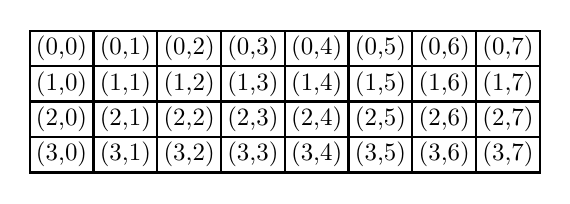
\begin{tikzpicture}[thick,scale=0.9, every node/.style={scale=0.9}]
      \foreach \row in {0,...,3} {
        \foreach \col in {0,...,7} {
          \draw (0.9*\col,-0.5*\row) rectangle ++(0.9,-0.5) node[pos=.5] {(\row,\col)};
        }
      }
    \end{tikzpicture}
    \subcaption{\tabular[t]{@{}l@{}}恒等坐标 \\ $(4,8):(e_0,e_1)$\endtabular}
    \label{fig:layouts:coord0}
\end{subfigure}
\begin{subfigure}[t]{0.45\textwidth}
    \centering
    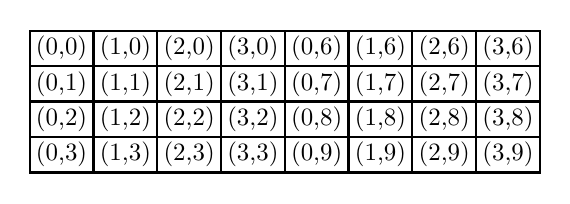
\begin{tikzpicture}[thick,scale=0.9, every node/.style={scale=0.9}]
      \foreach \row in {0,...,3} {
        \foreach \cola in {0,...,3} {
          \foreach \colb in {0,...,1} {
            \pgfmathtruncatemacro{\secondcoord}{\row + 6*\colb}
            \draw (0.9*\cola+3.6*\colb,-0.5*\row) rectangle ++(0.9,-0.5) node[pos=.5] {(\cola,\secondcoord)};
          }
        }
      }
    \end{tikzpicture}
    \subcaption{\tabular[t]{@{}l@{}}转置块状坐标 \\ $(4,(4,2)):(e_1,(e_0,6e_1))$\endtabular}
    \label{fig:layouts:coord1}
\end{subfigure}
%\begin{subfigure}[t]{0.7\textwidth}
%    \centering
%    \begin{tikzpicture}[thick,scale=0.9, every node/.style={scale=0.9}]
%      \foreach \row in {0,...,3} {
%        \foreach \col in {0,...,7} {
%          \pgfmathparse{int(mod(\row,2))}\let\i\pgfmathresult
%          \pgfmathparse{int(mod(\col,2))}\let\j\pgfmathresult
%          \pgfmathparse{int(int(\col/2) + 4*int(\row/2))}\let\k\pgfmathresult
%          \draw (1.3*\col,-0.5*\row) rectangle ++(1.3,-0.5) node[pos=.5] {(\i,\j,\k)};
%        }
%      }
%    \end{tikzpicture}
%    \caption{折叠坐标布局 \\ $((2,2),(2,4)):((e_0,4e_2),(e_1,e_2))$}
%\end{subfigure}
\begin{subfigure}[t]{0.45\textwidth}
    \centering
    \begin{tikzpicture}[thick,scale=1, every node/.style={scale=1}]
        \draw[step=0.5cm,color=black] (-3,-1) grid (3,1);
        \matrix[matrix of nodes,nodes={inner sep=0pt,text width=.5cm,align=center,minimum height=.5cm}]{
            0 & 5 & 10 & 15 & 16 & 21 & 26 & 31 & 32 & 37 & 42 & 47 \\
            1 & 4 & 11 & 14 & 17 & 20 & 27 & 30 & 33 & 36 & 43 & 46 \\
            2 & 7 &  8 & 13 & 18 & 23 & 24 & 29 & 34 & 39 & 40 & 45 \\
            3 & 6 &  9 & 12 & 19 & 22 & 25 & 28 & 35 & 38 & 41 & 44 \\};
        % \draw[line width=2pt,rounded corners,opacity=0.2]
        % (-1.75,+0.75) -- (-1.75,-0.75) --
        % (-1.25,+0.75) -- (-1.25,-0.75) --
        % (-0.75,+0.75) -- (-0.75,-0.75) --
        % (-0.25,+0.75) -- (-0.25,-0.75) --
        % (+0.25,+0.75) -- (+0.25,-0.75) --
        % (+0.75,+0.75) -- (+0.75,-0.75) --
        % (+1.25,+0.75) -- (+1.25,-0.75) --
        % (+1.75,+0.75) -- (+1.75,-0.75);
    \end{tikzpicture}
    \subcaption{\tabular[t]{@{}l@{}}二进制 Swizzle \\ $(4,(4,3)):(f_1,(f_5,f_{16}))$ \\ $f_i \in F_2 = (\Z,XOR,\cdot)$\endtabular}
    \label{fig:layouts:swizzle}
\end{subfigure}
\caption{以二维坐标绘制的布局示例。这些布局使用来自整数半模（integer-semimodule）的步幅来定义函数，这些函数在跟踪坐标以及按非仿射（non-affine）模式对偏移做“混淆（swizzle）”处理时非常有用。}
\label{fig:layouts2}
\end{figure}

图~\ref{fig:layouts2} 展示了用整数半模步幅而非整数步幅构造的布局示例。图~\ref{fig:layouts:coord0} 与图~\ref{fig:layouts:coord1} 演示了生成坐标的布局。在后续章节中我们将发现，这些坐标布局与其对应的数据布局对称地变换，并且常常作为检测数据张量越界访问并对其进行谓词化（predicating）的实用工具。此外，坐标张量已被证明对于 Hopper 与 Blackwell 中诸如 TMA 这类以坐标而非地址作为指令参数的指令非常有用。图~\ref{fig:layouts:swizzle} 使用了一个以二进制 XOR 替换群加法的整数半模。它可用于生成所谓的 swizzle 模式，这类模式有助于避免对共享内存读写访问模式中的 bank 冲突。这些示例突显了 \CuTe 布局概念的统一性以及它所能表示函数的普适性。

\wpssh{完备性}

任何满足 $f(0) = 0$ 且定义域为有限集合 $\Z_N$ 的函数 $f$ 都可以表示为有限个 \CuTe 布局的函数复合。这意味着 \CuTe 布局在函数复合下构成一个生成集。这样的函数 $f$ 可以表示为如下复合序列
\begin{align*}
f &\equiv (2,2,2,\ldots):(f(1),f(2),f(3),\ldots) \ \circ \ (3,1):(1,4) \ \circ \ (4,1):(1,6) \ \circ \ \cdots \ \circ \ (N-1,1):(1,2(N-2)).
\end{align*}
对所有 $i \in \Z_N / \{0\}$，最右边的 $N-3$ 个布局将 $i \to 2^{i-1}$，而最左边的布局将 $2^{i-1} \to f(i)$。注意，我们在上面求值中间布局时使用的是扩展定义域 $\Z$，而不是界内定义域 $\Z_N$。

\wpssh{半线性}

形状—步幅定义 $\v{L} = D \circ S$ 连同推广的整数模（integer-module）步幅，给出了布局函数一种特别有用的线性代数视角，
\begin{align}
\v{L}(c) = (D \circ S)(c) = d \cdot S(c) = d \cdot \tilde{c}.
\end{align}
形状函数是到自然坐标 $\tilde{c} \in \Z^S$ 的一个便利的半仿射双射，而步幅函数是自然坐标的线性函数。事实上，对于两个自然坐标 $\tilde{c}_0, \tilde{c}_1 \in \Z^S$，布局函数是线性（linear）的，
\begin{align*}
\v{L}(\alpha \tilde{c}_0 + \beta \tilde{c}_1) = d \cdot (\alpha \tilde{c}_0 + \beta \tilde{c}_1) = \alpha (d \cdot \tilde{c}_0) + \beta (d \cdot \tilde{c}_1) = \alpha \v{L}(\tilde{c}_0) + \beta \v{L}(\tilde{c}_1),
\end{align*}
因为形状函数是恒等映射且步幅函数是线性的。注意，对任意坐标 $c_0, c_1 \in \Z(S)$，布局不是线性的，因为形状函数不是线性的，
\begin{align*}
\tilde{c} = S(c_0 + c_1) \neq S(c_0) + S(c_1) = \tilde{c}_0 + \tilde{c}_1.
\end{align*}
因此，布局函数在自然坐标 $\tilde{c} \in \Z^S$ 下是线性的，但在任意坐标 $c \in \Z(S)$ 下是非线性的。

在自然坐标下，$d \cdot \tilde{c}$ 可以解释为推广的矩阵—向量乘积（matrix-vector product），
\begin{align*}
\v{L}(c) = d \cdot \tilde{c} = \v{D} \ \tilde{c}
\end{align*}
其中 $\v{D}$ 是元素取自某个整数半模 $\D$ 的矩阵。在最常见的整数步幅情形下，$\D = \Z$，这是 $\v{D} \in \Z^{1 \times n}$ 的矩阵—向量乘积。当步幅取自坐标整数半模 $\D = (\Z^S, +, \cdot)$ 时，这是 $\v{D} \in \Z^{m \times n}$ 的矩阵—向量乘积。当步幅是二进制序列时，$\D = F_2^m = (\Z_{2^m}, XOR, \cdot)$，这是 $\v{D} \in \mathbb{F}_2^{m \times n}$ 的矩阵—向量乘积。

\begin{table}[ht]
\begin{center}
\begin{tabular}{|>{$}c<{$}|>{$}c<{$}|c|}
\v{L} & \text{线性形式：} r = \v{D} \ \tilde{c} & 说明 \\ \hline \hline
((2,2),(4,\ 2)):((1,8),(2,16)) & r = \begin{bmatrix}1 & 8 & 2 & 16\end{bmatrix} \begin{bmatrix} \tilde{c}_0 \\ \tilde{c}_1 \\ \tilde{c}_2 \\ \tilde{c}_3 \end{bmatrix} & \shortstack{整数步幅是\\ $1 {\times} n$ $\Z$-矩阵的列} \\ \hline
(4,(4,2)):(e_1,(e_0,6e_1)) & \begin{bmatrix}r_0 \\ r_1\end{bmatrix} = \begin{bmatrix}0 & 1 & 0 \\ 1 & 0 & 6 \end{bmatrix} \begin{bmatrix} \tilde{c}_0 \\ \tilde{c}_1 \\ \tilde{c}_2 \end{bmatrix} &
\shortstack{坐标步幅是\\ $m {\times} n$ $\Z$-矩阵的列} \\ \hline
\shortstack{$(4,4) : (f_1,f_5)$ \\ $\equiv ((2,2),(2,2)):((f_1,f_2),(f_5,f_{10}))$} &
\footnotesize
\begin{bmatrix}r_0 \\ r_1 \\ r_2 \\ r_3\end{bmatrix} =
\begin{bmatrix}
1 & 0 & 1 & 0 \\
0 & 1 & 0 & 1 \\
0 & 0 & 1 & 0 \\
0 & 0 & 0 & 1 \\
\end{bmatrix}
\begin{bmatrix} \tilde{c}_0 \\ \tilde{c}_1 \\ \tilde{c}_2 \\ \tilde{c}_3 \end{bmatrix} &
\shortstack{二进制步幅是\\ $m {\times} n$ $\mathbb{F}_2$-矩阵的列} \\ \hline
\end{tabular}
\end{center}
\caption{布局及其对应的线性形式。}
\label{tab:linear_forms}
\end{table}

例如，表~\ref{tab:linear_forms} 展示了一个整数布局、一个坐标布局与一个二进制布局的线性形式。针对 $\mathbb{F}_2$ 线性形式已被充分研究的变换包括位排列补（Bit Permute Complement，BPC）与位矩阵乘补（Bit Matrix Multiply Complement，BMMC）变换（Edelman 等，1994；Cormen，1993；Bouverot-Dupuis 与 Sheeran，2023），它们近来在 SIMT GPU 编程中获得了重要的应用（Zhou 等，2025）。在这些工作中，所考虑的变换为
\begin{align}
f(\v{v}) = \v{A} \v{v} + \v{b}
\label{eqn:linear}
\end{align}
其中 $\v{A}$ 是一个 $m {\times} n$ 的二进制元素矩阵，$\v{v}$ 是长度为 $n$ 的二进制向量，$\v{b}$ 是长度为 $m$ 的二进制向量，且所有算术都以 2 为模（在只有两个元素的有限域 $\mathbb{F}_2$ 中）执行。

本文的后续章节将定义 \CuTe 布局上的代数运算，这些运算是从线性代数推广而来的。\CuTe 布局上的群复合可以解释为矩阵乘法的推广。\CuTe 布局的右逆与左逆可以解释为线性代数中的 Moore-Penrose 伪逆。事实上，在 BCP 与 BMMC 分析中也可以找到类似的线性代数表达式（Edelman 等，1994；Cormen，1993；Bouverot-Dupuis 与 Sheeran，2023；Zhou 等，2025），它们都在算法分析中使用分解、逆与矩阵乘积。\CuTe 布局代数可以解释为线性代数的 BCP 与 BMMC 运算向 $\mathbb{F}_2$ 域之外的推广。特别地，\CuTe 布局代数的主要动机来自张量异构数据布局中常见的一般整数步幅。在本工作中，我们旨在证明：这些运算更一般的函数式定义对 \CuTe 布局而言通常是可计算的，并且对广泛的分析与应用都是有用的。

%% wp3 张量与切片（论文 Tensor/Slicing 小节）
\wpsh{张量（Tensor）}
\label{sec:tensor}

最后，我们定义张量（tensor）——\CuTe 的核心对象——做法是把一个布局（layout）绑定到一个访问器（accessor）上。访问器实际上是面向布局的、支持随机访问的类指针对象。

\begin{definition}
{\em 访问器}（accessor）是支持偏移（offset）与解引用（dereference）操作的对象：
\begin{align*}
e + d &\to e', &&\text{将访问器 $e$ {\bf 偏移}（offset）$d \in \D$，产生另一访问器 $e'$；} \\
*e &\to v, &&\text{{\bf 解引用}（dereference）访问器 $e$，产生值 $v$；} \\
e[d] &\to *(e+d), &&\text{{\bf 下标}（subscript）算符，一种常用的便捷写法。}
\end{align*}
\end{definition}
当 $\D = \Z$ 时，访问器的常见实现包括原始指针（如 \texttt{T*}）、数组（如
\texttt{T[N]}）以及随机访问迭代器（如
\texttt{thrust::\allowbreak{}counting\allowbreak\_iterator} 与
\texttt{thrust::\allowbreak{}transform\allowbreak\_iterator} 等）。当 $\D$ 是更为特殊的整数半模时，访问器必须与该半群的加法运算相容。

\begin{definition}
{\em 张量}（tensor）由访问器 $e$ 与布局 $\v{L}$ 的复合（Composition）所定义，记作 $T = e \circ \v{L}$。张量对布局求值的方式是：把坐标 $c \in \Z(\v{L})$ 映射到陪域 $\D$，据此对访问器做偏移，再对结果解引用，从而得到张量的值。形式化地，
\begin{align}
T(c) = (e \circ \v{L})(c) = *(e + \v{L}(c)) = e[\v{L}(c)],
\label{eqn:tensor}
\end{align}
即得到张量在坐标 $c$ 处的值。
\end{definition}

大多数张量是以内存地址作为访问器的数据布局。例如，内存地址 $p$ 可以作为带普通偏移与解引用操作的指针访问器 $\{p\}$，用来构造数据张量，
\begin{align*}
\{p\} + b &\to \{p+b\} \\
*\{p\} &\to *p \\
T &= \{p\} \circ \v{L}.
\end{align*}
此外，图~\ref{fig:layouts} 中所示的所有布局都可以通过与计数迭代器 $\{a\}$ 复合而变换为隐式张量，该迭代器解引用到所存储的偏移 $a \in \Z$，
\begin{align*}
\{a\} + b &\to \{a+b\} \\
*\{a\} &\to a \\
T &= \{a\} \circ \v{L}.
\end{align*}
类似地，图~\ref{fig:layouts:coord0} 与图~\ref{fig:layouts:coord1} 中所示的坐标布局可以通过与访问器 $\{(a,b)\}$ 复合而变换为隐式张量，该访问器按坐标进行偏移，并解引用到所存储的坐标 $(a,b) \in \Z^{(\star,\star)}$，
\begin{align*}
\{(a,b)\} + (c,d) &\to \{(a+c,b+d)\} \\
*\{(a,b)\} &\to (a,b) \\
T &= \{(a,b)\} \circ \v{L}.
\end{align*}


% \wpssh{$\D$-torsor（$\D$-挠子）}

% 形式上，若集合 $E$ 配备运算 $E + M \to E$（其中 $M$ 是一个群），则称 $E$ 为一个 $M$-torsor。访问器是 $\D$-torsor，可以解引用到另一个集合 $V$，即其值集。例如，指针是一个 $\Z$-torsor，因为整数可以加到指针上得到另一个指针，而指针与指针相加则没有合理的含义。

\wpssh{切片（Slicing）}
\label{sec:slicing}

张量既可以被{\em 完全求值}，也可以通过{\em 切片}（slicing）进行{\em 部分求值}。由于 \CuTe 的 Tensor 可以视为带偏移的 Layout，因此可以沿自然坐标的任意一个或多个模进行任意切片。

\begin{itemize}[itemsep=0pt,topsep=2pt]
\item \textbf{完全求值}：用完整坐标 $c$ 应用式~\eqref{eqn:tensor}，得到一个值。
\item \textbf{部分求值（切片）}：当用不完整坐标 $c = c' + c^*$ 切片时（其中 $c^*$ 表示 $c$ 中未被指定的部分），结果是一个新张量。该操作表示为：
\begin{align}
T(c) = (e \circ \v{L})(c'+ c^*) = (e + \v{L}(c')) \circ \v{L}(c^*) = e' \circ \v{L}(c^*) = T'(c^*),
\end{align}
\end{itemize}
其中 $\v{L}(c')$ 可以被完全求值并累加进 $e$，而 $\v{L}(c^*)$ 是 $\v{L}$ 中尚未求值的子布局。切片产生一个子张量，可对其进一步求值或操作。

\begin{figure}[p]
\centering
\scalebox{0.6}{
\begin{tikzpicture}[x={(0cm,-1cm)},y={(1cm,0cm)},every node/.style={minimum size=1cm, outer sep=0pt}]
\node[fill=white] at (0,0) {\Large 0};
\node[fill=white] at (0,1) {\Large 2};
\node[fill=white] at (0,2) {\Large 15};
\node[fill=white] at (0,3) {\Large 17};
\node[fill=white] at (0,4) {\Large 30};
\node[fill=white] at (0,5) {\Large 32};
\node[fill=white] at (0,6) {\Large 100};
\node[fill=white] at (0,7) {\Large 102};
\node[fill=white] at (0,8) {\Large 115};
\node[fill=white] at (0,9) {\Large 117};
\node[fill=white] at (0,10) {\Large 130};
\node[fill=white] at (0,11) {\Large 132};
\node[fill=white] at (1,0) {\Large 4};
\node[fill=white] at (1,1) {\Large 6};
\node[fill=white] at (1,2) {\Large 19};
\node[fill=white] at (1,3) {\Large 21};
\node[fill=white] at (1,4) {\Large 34};
\node[fill=white] at (1,5) {\Large 36};
\node[fill=white] at (1,6) {\Large 104};
\node[fill=white] at (1,7) {\Large 106};
\node[fill=white] at (1,8) {\Large 119};
\node[fill=white] at (1,9) {\Large 121};
\node[fill=white] at (1,10) {\Large 134};
\node[fill=white] at (1,11) {\Large 136};
\node[fill=white] at (2,0) {\Large 8};
\node[fill=white] at (2,1) {\Large 10};
\node[fill=white] at (2,2) {\Large 23};
\node[fill=white] at (2,3) {\Large 25};
\node[fill=white] at (2,4) {\Large 38};
\node[fill=white] at (2,5) {\Large 40};
\node[fill=white] at (2,6) {\Large 108};
\node[fill=white] at (2,7) {\Large 110};
\node[fill=white] at (2,8) {\Large 123};
\node[fill=white] at (2,9) {\Large 125};
\node[fill=white] at (2,10) {\Large 138};
\node[fill=white] at (2,11) {\Large 140};
\node[fill=white] at (3,0) {\Large 1};
\node[fill=white] at (3,1) {\Large 3};
\node[fill=white] at (3,2) {\Large 16};
\node[fill=white] at (3,3) {\Large 18};
\node[fill=white] at (3,4) {\Large 31};
\node[fill=white] at (3,5) {\Large 33};
\node[fill=white] at (3,6) {\Large 101};
\node[fill=white] at (3,7) {\Large 103};
\node[fill=white] at (3,8) {\Large 116};
\node[fill=white] at (3,9) {\Large 118};
\node[fill=white] at (3,10) {\Large 131};
\node[fill=white] at (3,11) {\Large 133};
\node[fill=white] at (4,0) {\Large 5};
\node[fill=white] at (4,1) {\Large 7};
\node[fill=white] at (4,2) {\Large 20};
\node[fill=white] at (4,3) {\Large 22};
\node[fill=white] at (4,4) {\Large 35};
\node[fill=white] at (4,5) {\Large 37};
\node[fill=white] at (4,6) {\Large 105};
\node[fill=white] at (4,7) {\Large 107};
\node[fill=white] at (4,8) {\Large 120};
\node[fill=white] at (4,9) {\Large 122};
\node[fill=white] at (4,10) {\Large 135};
\node[fill=white] at (4,11) {\Large 137};
\node[fill=white] at (5,0) {\Large 9};
\node[fill=white] at (5,1) {\Large 11};
\node[fill=white] at (5,2) {\Large 24};
\node[fill=white] at (5,3) {\Large 26};
\node[fill=white] at (5,4) {\Large 39};
\node[fill=white] at (5,5) {\Large 41};
\node[fill=white] at (5,6) {\Large 109};
\node[fill=white] at (5,7) {\Large 111};
\node[fill=white] at (5,8) {\Large 124};
\node[fill=white] at (5,9) {\Large 126};
\node[fill=white] at (5,10) {\Large 139};
\node[fill=white] at (5,11) {\Large 141};
\draw[color=black,thick,shift={(-0.5,-0.5)}] (0,0) grid (6,12);
\node at (0,-1) {\Large{\texttt{0}}};
\node at (1,-1) {\Large{\texttt{1}}};
\node at (2,-1) {\Large{\texttt{2}}};
\node at (3,-1) {\Large{\texttt{3}}};
\node at (4,-1) {\Large{\texttt{4}}};
\node at (5,-1) {\Large{\texttt{5}}};
\node at (-1,0) {\Large{\texttt{0}}};
\node at (-1,1) {\Large{\texttt{1}}};
\node at (-1,2) {\Large{\texttt{2}}};
\node at (-1,3) {\Large{\texttt{3}}};
\node at (-1,4) {\Large{\texttt{4}}};
\node at (-1,5) {\Large{\texttt{5}}};
\node at (-1,6) {\Large{\texttt{6}}};
\node at (-1,7) {\Large{\texttt{7}}};
\node at (-1,8) {\Large{\texttt{8}}};
\node at (-1,9) {\Large{\texttt{9}}};
\node at (-1,10) {\Large{\texttt{10}}};
\node at (-1,11) {\Large{\texttt{11}}};
\node at (6.25,5.5) {\huge 张量 $\v{A} = \{0\} \circ ((3,2),((2,3),2)):((4,1),((2,15),100))$};
\end{tikzpicture}
}\\
\vspace{1em}
\begin{tabular}{|>{\centering\arraybackslash}m{3.6cm}|>{\centering\arraybackslash}m{4.7cm}|>{\centering\arraybackslash}m{4.7cm}|}
切片 & 切片后的张量 & 切片示意图 \\
\hline\hline
$\v{A}(2,\_)$ & $\{8\} \circ ((2,3),2):((2,15),100)$ &
\scalebox{0.4}{
\begin{adjustbox}{margin=0.5cm}
\scalebox{0.8}{
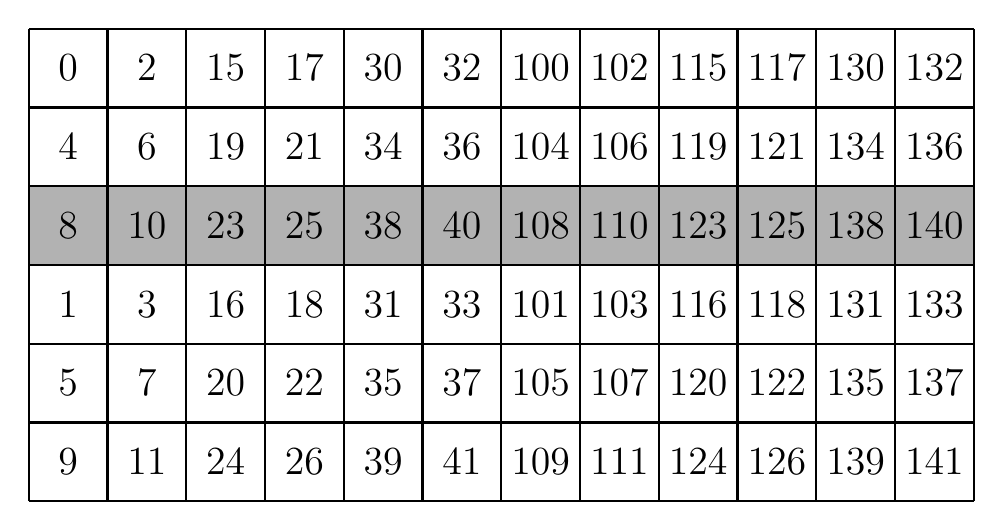
\begin{tikzpicture}[x={(0cm,-1cm)},y={(1cm,0cm)},every node/.style={minimum size=1cm, outer sep=0pt}]
\node[fill=white] at (0,0) {\Large 0};
\node[fill=white] at (0,1) {\Large 2};
\node[fill=white] at (0,2) {\Large 15};
\node[fill=white] at (0,3) {\Large 17};
\node[fill=white] at (0,4) {\Large 30};
\node[fill=white] at (0,5) {\Large 32};
\node[fill=white] at (0,6) {\Large 100};
\node[fill=white] at (0,7) {\Large 102};
\node[fill=white] at (0,8) {\Large 115};
\node[fill=white] at (0,9) {\Large 117};
\node[fill=white] at (0,10) {\Large 130};
\node[fill=white] at (0,11) {\Large 132};
\node[fill=white] at (1,0) {\Large 4};
\node[fill=white] at (1,1) {\Large 6};
\node[fill=white] at (1,2) {\Large 19};
\node[fill=white] at (1,3) {\Large 21};
\node[fill=white] at (1,4) {\Large 34};
\node[fill=white] at (1,5) {\Large 36};
\node[fill=white] at (1,6) {\Large 104};
\node[fill=white] at (1,7) {\Large 106};
\node[fill=white] at (1,8) {\Large 119};
\node[fill=white] at (1,9) {\Large 121};
\node[fill=white] at (1,10) {\Large 134};
\node[fill=white] at (1,11) {\Large 136};
\node[fill=black!30] at (2,0) {\Large 8};
\node[fill=black!30] at (2,1) {\Large 10};
\node[fill=black!30] at (2,2) {\Large 23};
\node[fill=black!30] at (2,3) {\Large 25};
\node[fill=black!30] at (2,4) {\Large 38};
\node[fill=black!30] at (2,5) {\Large 40};
\node[fill=black!30] at (2,6) {\Large 108};
\node[fill=black!30] at (2,7) {\Large 110};
\node[fill=black!30] at (2,8) {\Large 123};
\node[fill=black!30] at (2,9) {\Large 125};
\node[fill=black!30] at (2,10) {\Large 138};
\node[fill=black!30] at (2,11) {\Large 140};
\node[fill=white] at (3,0) {\Large 1};
\node[fill=white] at (3,1) {\Large 3};
\node[fill=white] at (3,2) {\Large 16};
\node[fill=white] at (3,3) {\Large 18};
\node[fill=white] at (3,4) {\Large 31};
\node[fill=white] at (3,5) {\Large 33};
\node[fill=white] at (3,6) {\Large 101};
\node[fill=white] at (3,7) {\Large 103};
\node[fill=white] at (3,8) {\Large 116};
\node[fill=white] at (3,9) {\Large 118};
\node[fill=white] at (3,10) {\Large 131};
\node[fill=white] at (3,11) {\Large 133};
\node[fill=white] at (4,0) {\Large 5};
\node[fill=white] at (4,1) {\Large 7};
\node[fill=white] at (4,2) {\Large 20};
\node[fill=white] at (4,3) {\Large 22};
\node[fill=white] at (4,4) {\Large 35};
\node[fill=white] at (4,5) {\Large 37};
\node[fill=white] at (4,6) {\Large 105};
\node[fill=white] at (4,7) {\Large 107};
\node[fill=white] at (4,8) {\Large 120};
\node[fill=white] at (4,9) {\Large 122};
\node[fill=white] at (4,10) {\Large 135};
\node[fill=white] at (4,11) {\Large 137};
\node[fill=white] at (5,0) {\Large 9};
\node[fill=white] at (5,1) {\Large 11};
\node[fill=white] at (5,2) {\Large 24};
\node[fill=white] at (5,3) {\Large 26};
\node[fill=white] at (5,4) {\Large 39};
\node[fill=white] at (5,5) {\Large 41};
\node[fill=white] at (5,6) {\Large 109};
\node[fill=white] at (5,7) {\Large 111};
\node[fill=white] at (5,8) {\Large 124};
\node[fill=white] at (5,9) {\Large 126};
\node[fill=white] at (5,10) {\Large 139};
\node[fill=white] at (5,11) {\Large 141};
\draw[color=black,thick,shift={(-0.5,-0.5)}] (0,0) grid (6,12);
\end{tikzpicture}
}
\end{adjustbox}
} \\
\hline
$\v{A}(\_,5)$ & $\{32\} \circ (3,2):(4,1)$ &
\scalebox{0.4}{
\begin{adjustbox}{margin=0.5cm}
\scalebox{0.8}{
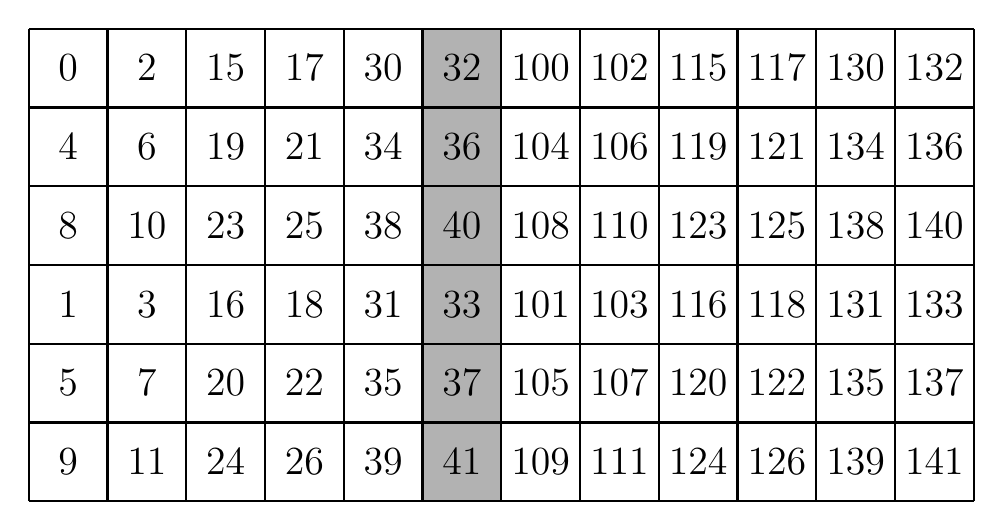
\begin{tikzpicture}[x={(0cm,-1cm)},y={(1cm,0cm)},every node/.style={minimum size=1cm, outer sep=0pt}]
\node[fill=white] at (0,0) {\Large 0};
\node[fill=white] at (0,1) {\Large 2};
\node[fill=white] at (0,2) {\Large 15};
\node[fill=white] at (0,3) {\Large 17};
\node[fill=white] at (0,4) {\Large 30};
\node[fill=black!30] at (0,5) {\Large 32};
\node[fill=white] at (0,6) {\Large 100};
\node[fill=white] at (0,7) {\Large 102};
\node[fill=white] at (0,8) {\Large 115};
\node[fill=white] at (0,9) {\Large 117};
\node[fill=white] at (0,10) {\Large 130};
\node[fill=white] at (0,11) {\Large 132};
\node[fill=white] at (1,0) {\Large 4};
\node[fill=white] at (1,1) {\Large 6};
\node[fill=white] at (1,2) {\Large 19};
\node[fill=white] at (1,3) {\Large 21};
\node[fill=white] at (1,4) {\Large 34};
\node[fill=black!30] at (1,5) {\Large 36};
\node[fill=white] at (1,6) {\Large 104};
\node[fill=white] at (1,7) {\Large 106};
\node[fill=white] at (1,8) {\Large 119};
\node[fill=white] at (1,9) {\Large 121};
\node[fill=white] at (1,10) {\Large 134};
\node[fill=white] at (1,11) {\Large 136};
\node[fill=white] at (2,0) {\Large 8};
\node[fill=white] at (2,1) {\Large 10};
\node[fill=white] at (2,2) {\Large 23};
\node[fill=white] at (2,3) {\Large 25};
\node[fill=white] at (2,4) {\Large 38};
\node[fill=black!30] at (2,5) {\Large 40};
\node[fill=white] at (2,6) {\Large 108};
\node[fill=white] at (2,7) {\Large 110};
\node[fill=white] at (2,8) {\Large 123};
\node[fill=white] at (2,9) {\Large 125};
\node[fill=white] at (2,10) {\Large 138};
\node[fill=white] at (2,11) {\Large 140};
\node[fill=white] at (3,0) {\Large 1};
\node[fill=white] at (3,1) {\Large 3};
\node[fill=white] at (3,2) {\Large 16};
\node[fill=white] at (3,3) {\Large 18};
\node[fill=white] at (3,4) {\Large 31};
\node[fill=black!30] at (3,5) {\Large 33};
\node[fill=white] at (3,6) {\Large 101};
\node[fill=white] at (3,7) {\Large 103};
\node[fill=white] at (3,8) {\Large 116};
\node[fill=white] at (3,9) {\Large 118};
\node[fill=white] at (3,10) {\Large 131};
\node[fill=white] at (3,11) {\Large 133};
\node[fill=white] at (4,0) {\Large 5};
\node[fill=white] at (4,1) {\Large 7};
\node[fill=white] at (4,2) {\Large 20};
\node[fill=white] at (4,3) {\Large 22};
\node[fill=white] at (4,4) {\Large 35};
\node[fill=black!30] at (4,5) {\Large 37};
\node[fill=white] at (4,6) {\Large 105};
\node[fill=white] at (4,7) {\Large 107};
\node[fill=white] at (4,8) {\Large 120};
\node[fill=white] at (4,9) {\Large 122};
\node[fill=white] at (4,10) {\Large 135};
\node[fill=white] at (4,11) {\Large 137};
\node[fill=white] at (5,0) {\Large 9};
\node[fill=white] at (5,1) {\Large 11};
\node[fill=white] at (5,2) {\Large 24};
\node[fill=white] at (5,3) {\Large 26};
\node[fill=white] at (5,4) {\Large 39};
\node[fill=black!30] at (5,5) {\Large 41};
\node[fill=white] at (5,6) {\Large 109};
\node[fill=white] at (5,7) {\Large 111};
\node[fill=white] at (5,8) {\Large 124};
\node[fill=white] at (5,9) {\Large 126};
\node[fill=white] at (5,10) {\Large 139};
\node[fill=white] at (5,11) {\Large 141};
\draw[color=black,thick,shift={(-0.5,-0.5)}] (0,0) grid (6,12);
\end{tikzpicture}
}
\end{adjustbox}
} \\
\hline
$\v{A}(2,((0,\_),\_))$ & $\{8\} \circ (3,2):(15,100)$ &
\scalebox{0.4}{
\begin{adjustbox}{margin=0.5cm}
\scalebox{0.8}{
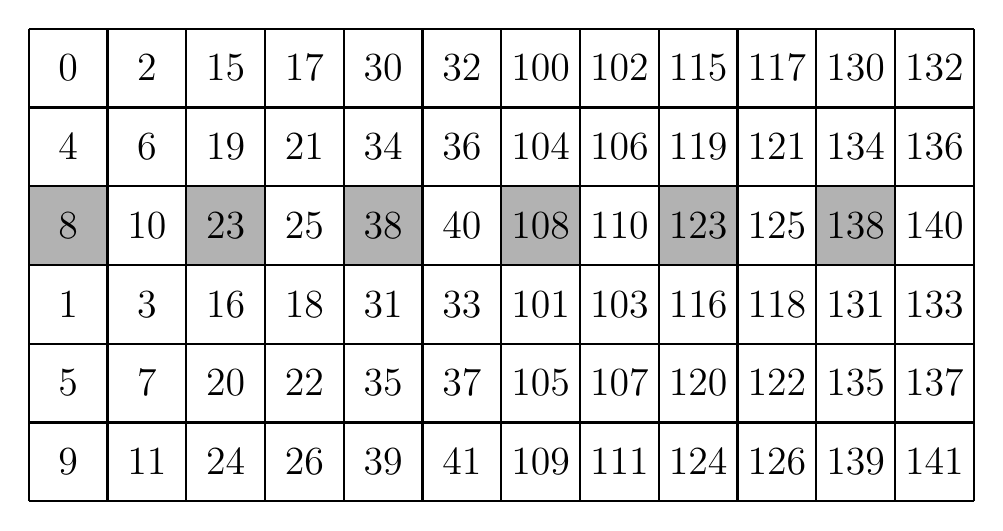
\begin{tikzpicture}[x={(0cm,-1cm)},y={(1cm,0cm)},every node/.style={minimum size=1cm, outer sep=0pt}]
\node[fill=white] at (0,0) {\Large 0};
\node[fill=white] at (0,1) {\Large 2};
\node[fill=white] at (0,2) {\Large 15};
\node[fill=white] at (0,3) {\Large 17};
\node[fill=white] at (0,4) {\Large 30};
\node[fill=white] at (0,5) {\Large 32};
\node[fill=white] at (0,6) {\Large 100};
\node[fill=white] at (0,7) {\Large 102};
\node[fill=white] at (0,8) {\Large 115};
\node[fill=white] at (0,9) {\Large 117};
\node[fill=white] at (0,10) {\Large 130};
\node[fill=white] at (0,11) {\Large 132};
\node[fill=white] at (1,0) {\Large 4};
\node[fill=white] at (1,1) {\Large 6};
\node[fill=white] at (1,2) {\Large 19};
\node[fill=white] at (1,3) {\Large 21};
\node[fill=white] at (1,4) {\Large 34};
\node[fill=white] at (1,5) {\Large 36};
\node[fill=white] at (1,6) {\Large 104};
\node[fill=white] at (1,7) {\Large 106};
\node[fill=white] at (1,8) {\Large 119};
\node[fill=white] at (1,9) {\Large 121};
\node[fill=white] at (1,10) {\Large 134};
\node[fill=white] at (1,11) {\Large 136};
\node[fill=black!30] at (2,0) {\Large 8};
\node[fill=white] at (2,1) {\Large 10};
\node[fill=black!30] at (2,2) {\Large 23};
\node[fill=white] at (2,3) {\Large 25};
\node[fill=black!30] at (2,4) {\Large 38};
\node[fill=white] at (2,5) {\Large 40};
\node[fill=black!30] at (2,6) {\Large 108};
\node[fill=white] at (2,7) {\Large 110};
\node[fill=black!30] at (2,8) {\Large 123};
\node[fill=white] at (2,9) {\Large 125};
\node[fill=black!30] at (2,10) {\Large 138};
\node[fill=white] at (2,11) {\Large 140};
\node[fill=white] at (3,0) {\Large 1};
\node[fill=white] at (3,1) {\Large 3};
\node[fill=white] at (3,2) {\Large 16};
\node[fill=white] at (3,3) {\Large 18};
\node[fill=white] at (3,4) {\Large 31};
\node[fill=white] at (3,5) {\Large 33};
\node[fill=white] at (3,6) {\Large 101};
\node[fill=white] at (3,7) {\Large 103};
\node[fill=white] at (3,8) {\Large 116};
\node[fill=white] at (3,9) {\Large 118};
\node[fill=white] at (3,10) {\Large 131};
\node[fill=white] at (3,11) {\Large 133};
\node[fill=white] at (4,0) {\Large 5};
\node[fill=white] at (4,1) {\Large 7};
\node[fill=white] at (4,2) {\Large 20};
\node[fill=white] at (4,3) {\Large 22};
\node[fill=white] at (4,4) {\Large 35};
\node[fill=white] at (4,5) {\Large 37};
\node[fill=white] at (4,6) {\Large 105};
\node[fill=white] at (4,7) {\Large 107};
\node[fill=white] at (4,8) {\Large 120};
\node[fill=white] at (4,9) {\Large 122};
\node[fill=white] at (4,10) {\Large 135};
\node[fill=white] at (4,11) {\Large 137};
\node[fill=white] at (5,0) {\Large 9};
\node[fill=white] at (5,1) {\Large 11};
\node[fill=white] at (5,2) {\Large 24};
\node[fill=white] at (5,3) {\Large 26};
\node[fill=white] at (5,4) {\Large 39};
\node[fill=white] at (5,5) {\Large 41};
\node[fill=white] at (5,6) {\Large 109};
\node[fill=white] at (5,7) {\Large 111};
\node[fill=white] at (5,8) {\Large 124};
\node[fill=white] at (5,9) {\Large 126};
\node[fill=white] at (5,10) {\Large 139};
\node[fill=white] at (5,11) {\Large 141};
\draw[color=black,thick,shift={(-0.5,-0.5)}] (0,0) grid (6,12);
\end{tikzpicture}
}
\end{adjustbox}
} \\
\hline
$\v{A}((\_,1),(\_,0))$ & $\{1\} \circ (3,(2,3)):(4,(2,15))$ &
\scalebox{0.4}{
\begin{adjustbox}{margin=0.5cm}
\scalebox{0.8}{
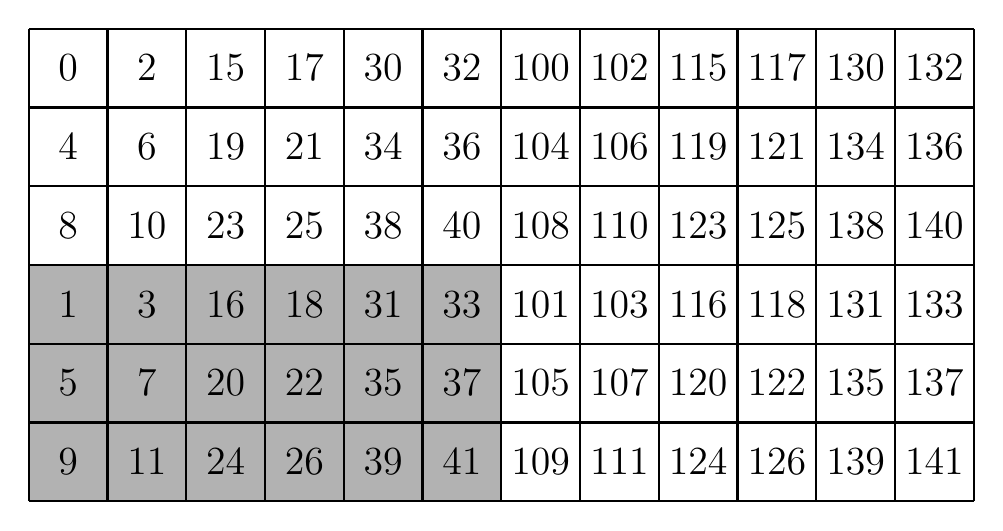
\begin{tikzpicture}[x={(0cm,-1cm)},y={(1cm,0cm)},every node/.style={minimum size=1cm, outer sep=0pt}]
\node[fill=white] at (0,0) {\Large 0};
\node[fill=white] at (0,1) {\Large 2};
\node[fill=white] at (0,2) {\Large 15};
\node[fill=white] at (0,3) {\Large 17};
\node[fill=white] at (0,4) {\Large 30};
\node[fill=white] at (0,5) {\Large 32};
\node[fill=white] at (0,6) {\Large 100};
\node[fill=white] at (0,7) {\Large 102};
\node[fill=white] at (0,8) {\Large 115};
\node[fill=white] at (0,9) {\Large 117};
\node[fill=white] at (0,10) {\Large 130};
\node[fill=white] at (0,11) {\Large 132};
\node[fill=white] at (1,0) {\Large 4};
\node[fill=white] at (1,1) {\Large 6};
\node[fill=white] at (1,2) {\Large 19};
\node[fill=white] at (1,3) {\Large 21};
\node[fill=white] at (1,4) {\Large 34};
\node[fill=white] at (1,5) {\Large 36};
\node[fill=white] at (1,6) {\Large 104};
\node[fill=white] at (1,7) {\Large 106};
\node[fill=white] at (1,8) {\Large 119};
\node[fill=white] at (1,9) {\Large 121};
\node[fill=white] at (1,10) {\Large 134};
\node[fill=white] at (1,11) {\Large 136};
\node[fill=white] at (2,0) {\Large 8};
\node[fill=white] at (2,1) {\Large 10};
\node[fill=white] at (2,2) {\Large 23};
\node[fill=white] at (2,3) {\Large 25};
\node[fill=white] at (2,4) {\Large 38};
\node[fill=white] at (2,5) {\Large 40};
\node[fill=white] at (2,6) {\Large 108};
\node[fill=white] at (2,7) {\Large 110};
\node[fill=white] at (2,8) {\Large 123};
\node[fill=white] at (2,9) {\Large 125};
\node[fill=white] at (2,10) {\Large 138};
\node[fill=white] at (2,11) {\Large 140};
\node[fill=black!30] at (3,0) {\Large 1};
\node[fill=black!30] at (3,1) {\Large 3};
\node[fill=black!30] at (3,2) {\Large 16};
\node[fill=black!30] at (3,3) {\Large 18};
\node[fill=black!30] at (3,4) {\Large 31};
\node[fill=black!30] at (3,5) {\Large 33};
\node[fill=white] at (3,6) {\Large 101};
\node[fill=white] at (3,7) {\Large 103};
\node[fill=white] at (3,8) {\Large 116};
\node[fill=white] at (3,9) {\Large 118};
\node[fill=white] at (3,10) {\Large 131};
\node[fill=white] at (3,11) {\Large 133};
\node[fill=black!30] at (4,0) {\Large 5};
\node[fill=black!30] at (4,1) {\Large 7};
\node[fill=black!30] at (4,2) {\Large 20};
\node[fill=black!30] at (4,3) {\Large 22};
\node[fill=black!30] at (4,4) {\Large 35};
\node[fill=black!30] at (4,5) {\Large 37};
\node[fill=white] at (4,6) {\Large 105};
\node[fill=white] at (4,7) {\Large 107};
\node[fill=white] at (4,8) {\Large 120};
\node[fill=white] at (4,9) {\Large 122};
\node[fill=white] at (4,10) {\Large 135};
\node[fill=white] at (4,11) {\Large 137};
\node[fill=black!30] at (5,0) {\Large 9};
\node[fill=black!30] at (5,1) {\Large 11};
\node[fill=black!30] at (5,2) {\Large 24};
\node[fill=black!30] at (5,3) {\Large 26};
\node[fill=black!30] at (5,4) {\Large 39};
\node[fill=black!30] at (5,5) {\Large 41};
\node[fill=white] at (5,6) {\Large 109};
\node[fill=white] at (5,7) {\Large 111};
\node[fill=white] at (5,8) {\Large 124};
\node[fill=white] at (5,9) {\Large 126};
\node[fill=white] at (5,10) {\Large 139};
\node[fill=white] at (5,11) {\Large 141};
\draw[color=black,thick,shift={(-0.5,-0.5)}] (0,0) grid (6,12);
\end{tikzpicture}
}
\end{adjustbox}
} \\
\hline
$\v{A}((\_,0),((0,\_),1))$ & $\{100\} \circ (3,3):(4,15)$ &
\scalebox{0.4}{
\begin{adjustbox}{margin=0.5cm}
\scalebox{0.8}{
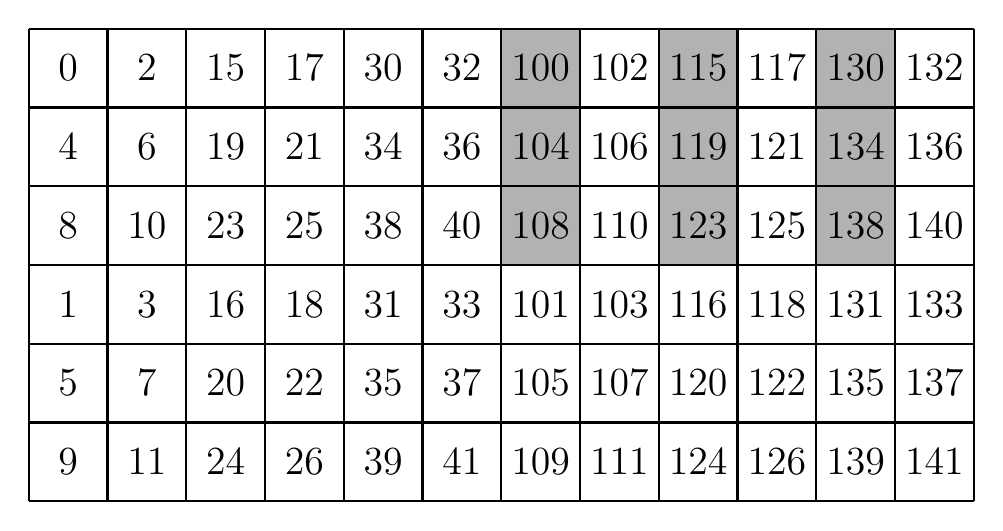
\begin{tikzpicture}[x={(0cm,-1cm)},y={(1cm,0cm)},every node/.style={minimum size=1cm, outer sep=0pt}]
\node[fill=white] at (0,0) {\Large 0};
\node[fill=white] at (0,1) {\Large 2};
\node[fill=white] at (0,2) {\Large 15};
\node[fill=white] at (0,3) {\Large 17};
\node[fill=white] at (0,4) {\Large 30};
\node[fill=white] at (0,5) {\Large 32};
\node[fill=black!30] at (0,6) {\Large 100};
\node[fill=white] at (0,7) {\Large 102};
\node[fill=black!30] at (0,8) {\Large 115};
\node[fill=white] at (0,9) {\Large 117};
\node[fill=black!30] at (0,10) {\Large 130};
\node[fill=white] at (0,11) {\Large 132};
\node[fill=white] at (1,0) {\Large 4};
\node[fill=white] at (1,1) {\Large 6};
\node[fill=white] at (1,2) {\Large 19};
\node[fill=white] at (1,3) {\Large 21};
\node[fill=white] at (1,4) {\Large 34};
\node[fill=white] at (1,5) {\Large 36};
\node[fill=black!30] at (1,6) {\Large 104};
\node[fill=white] at (1,7) {\Large 106};
\node[fill=black!30] at (1,8) {\Large 119};
\node[fill=white] at (1,9) {\Large 121};
\node[fill=black!30] at (1,10) {\Large 134};
\node[fill=white] at (1,11) {\Large 136};
\node[fill=white] at (2,0) {\Large 8};
\node[fill=white] at (2,1) {\Large 10};
\node[fill=white] at (2,2) {\Large 23};
\node[fill=white] at (2,3) {\Large 25};
\node[fill=white] at (2,4) {\Large 38};
\node[fill=white] at (2,5) {\Large 40};
\node[fill=black!30] at (2,6) {\Large 108};
\node[fill=white] at (2,7) {\Large 110};
\node[fill=black!30] at (2,8) {\Large 123};
\node[fill=white] at (2,9) {\Large 125};
\node[fill=black!30] at (2,10) {\Large 138};
\node[fill=white] at (2,11) {\Large 140};
\node[fill=white] at (3,0) {\Large 1};
\node[fill=white] at (3,1) {\Large 3};
\node[fill=white] at (3,2) {\Large 16};
\node[fill=white] at (3,3) {\Large 18};
\node[fill=white] at (3,4) {\Large 31};
\node[fill=white] at (3,5) {\Large 33};
\node[fill=white] at (3,6) {\Large 101};
\node[fill=white] at (3,7) {\Large 103};
\node[fill=white] at (3,8) {\Large 116};
\node[fill=white] at (3,9) {\Large 118};
\node[fill=white] at (3,10) {\Large 131};
\node[fill=white] at (3,11) {\Large 133};
\node[fill=white] at (4,0) {\Large 5};
\node[fill=white] at (4,1) {\Large 7};
\node[fill=white] at (4,2) {\Large 20};
\node[fill=white] at (4,3) {\Large 22};
\node[fill=white] at (4,4) {\Large 35};
\node[fill=white] at (4,5) {\Large 37};
\node[fill=white] at (4,6) {\Large 105};
\node[fill=white] at (4,7) {\Large 107};
\node[fill=white] at (4,8) {\Large 120};
\node[fill=white] at (4,9) {\Large 122};
\node[fill=white] at (4,10) {\Large 135};
\node[fill=white] at (4,11) {\Large 137};
\node[fill=white] at (5,0) {\Large 9};
\node[fill=white] at (5,1) {\Large 11};
\node[fill=white] at (5,2) {\Large 24};
\node[fill=white] at (5,3) {\Large 26};
\node[fill=white] at (5,4) {\Large 39};
\node[fill=white] at (5,5) {\Large 41};
\node[fill=white] at (5,6) {\Large 109};
\node[fill=white] at (5,7) {\Large 111};
\node[fill=white] at (5,8) {\Large 124};
\node[fill=white] at (5,9) {\Large 126};
\node[fill=white] at (5,10) {\Large 139};
\node[fill=white] at (5,11) {\Large 141};
\draw[color=black,thick,shift={(-0.5,-0.5)}] (0,0) grid (6,12);
\end{tikzpicture}
}
\end{adjustbox}
} \\
\hline
$\v{A}((1,\_),((\_,0),\_))$ & $\{4\} \circ (2,(2,2)):(1,(2,100))$ &
\scalebox{0.4}{
\begin{adjustbox}{margin=0.5cm}
\scalebox{0.8}{
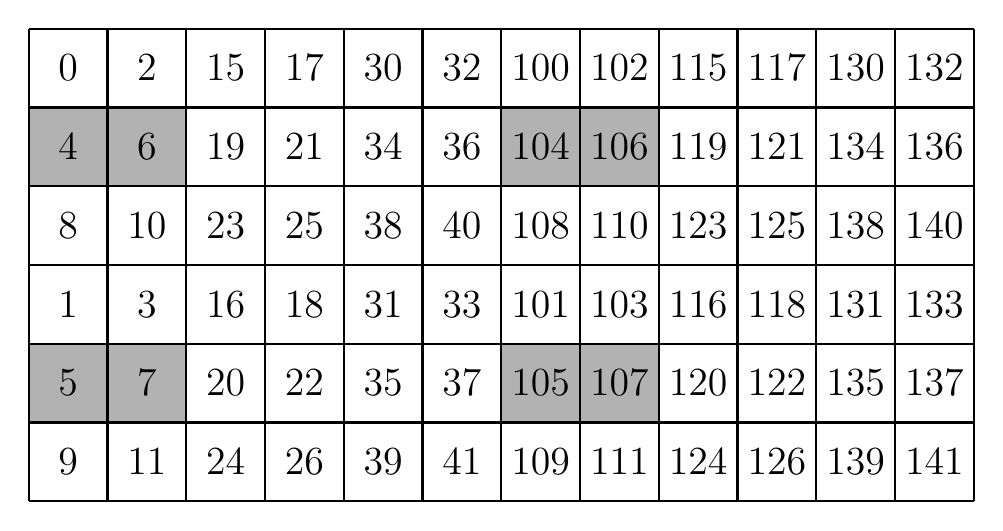
\begin{tikzpicture}[x={(0cm,-1cm)},y={(1cm,0cm)},every node/.style={minimum size=1cm, outer sep=0pt}]
\node[fill=white] at (0,0) {\Large 0};
\node[fill=white] at (0,1) {\Large 2};
\node[fill=white] at (0,2) {\Large 15};
\node[fill=white] at (0,3) {\Large 17};
\node[fill=white] at (0,4) {\Large 30};
\node[fill=white] at (0,5) {\Large 32};
\node[fill=white] at (0,6) {\Large 100};
\node[fill=white] at (0,7) {\Large 102};
\node[fill=white] at (0,8) {\Large 115};
\node[fill=white] at (0,9) {\Large 117};
\node[fill=white] at (0,10) {\Large 130};
\node[fill=white] at (0,11) {\Large 132};
\node[fill=black!30] at (1,0) {\Large 4};
\node[fill=black!30] at (1,1) {\Large 6};
\node[fill=white] at (1,2) {\Large 19};
\node[fill=white] at (1,3) {\Large 21};
\node[fill=white] at (1,4) {\Large 34};
\node[fill=white] at (1,5) {\Large 36};
\node[fill=black!30] at (1,6) {\Large 104};
\node[fill=black!30] at (1,7) {\Large 106};
\node[fill=white] at (1,8) {\Large 119};
\node[fill=white] at (1,9) {\Large 121};
\node[fill=white] at (1,10) {\Large 134};
\node[fill=white] at (1,11) {\Large 136};
\node[fill=white] at (2,0) {\Large 8};
\node[fill=white] at (2,1) {\Large 10};
\node[fill=white] at (2,2) {\Large 23};
\node[fill=white] at (2,3) {\Large 25};
\node[fill=white] at (2,4) {\Large 38};
\node[fill=white] at (2,5) {\Large 40};
\node[fill=white] at (2,6) {\Large 108};
\node[fill=white] at (2,7) {\Large 110};
\node[fill=white] at (2,8) {\Large 123};
\node[fill=white] at (2,9) {\Large 125};
\node[fill=white] at (2,10) {\Large 138};
\node[fill=white] at (2,11) {\Large 140};
\node[fill=white] at (3,0) {\Large 1};
\node[fill=white] at (3,1) {\Large 3};
\node[fill=white] at (3,2) {\Large 16};
\node[fill=white] at (3,3) {\Large 18};
\node[fill=white] at (3,4) {\Large 31};
\node[fill=white] at (3,5) {\Large 33};
\node[fill=white] at (3,6) {\Large 101};
\node[fill=white] at (3,7) {\Large 103};
\node[fill=white] at (3,8) {\Large 116};
\node[fill=white] at (3,9) {\Large 118};
\node[fill=white] at (3,10) {\Large 131};
\node[fill=white] at (3,11) {\Large 133};
\node[fill=black!30] at (4,0) {\Large 5};
\node[fill=black!30] at (4,1) {\Large 7};
\node[fill=white] at (4,2) {\Large 20};
\node[fill=white] at (4,3) {\Large 22};
\node[fill=white] at (4,4) {\Large 35};
\node[fill=white] at (4,5) {\Large 37};
\node[fill=black!30] at (4,6) {\Large 105};
\node[fill=black!30] at (4,7) {\Large 107};
\node[fill=white] at (4,8) {\Large 120};
\node[fill=white] at (4,9) {\Large 122};
\node[fill=white] at (4,10) {\Large 135};
\node[fill=white] at (4,11) {\Large 137};
\node[fill=white] at (5,0) {\Large 9};
\node[fill=white] at (5,1) {\Large 11};
\node[fill=white] at (5,2) {\Large 24};
\node[fill=white] at (5,3) {\Large 26};
\node[fill=white] at (5,4) {\Large 39};
\node[fill=white] at (5,5) {\Large 41};
\node[fill=white] at (5,6) {\Large 109};
\node[fill=white] at (5,7) {\Large 111};
\node[fill=white] at (5,8) {\Large 124};
\node[fill=white] at (5,9) {\Large 126};
\node[fill=white] at (5,10) {\Large 139};
\node[fill=white] at (5,11) {\Large 141};
\draw[color=black,thick,shift={(-0.5,-0.5)}] (0,0) grid (6,12);
\end{tikzpicture}
}
\end{adjustbox}
} \\
\hline
\end{tabular}
\caption{沿逻辑子边界切片以提取子张量的 $6 {\times} 12$ 张量。}
\label{fig:slicing}
\end{figure}

图~\ref{fig:slicing} 展示了在一个 $6 {\times} 12$ 矩阵中切片以提取行、列与子矩阵的示例。这些示例使用记号 $\{a\}$ 表示的计数迭代器访问器，以指明偏移 $a \in \Z$。切片的过程包括向张量偏移做累加，并确定布局中尚未求值的部分。

在许多张量库（如 {\tt numpy.ndarray}、{\tt torch.tensor} 和 MATLAB）中，切片以与上面类似的记法得到支持：写 {\tt my\_matrix[2,:]} 提取矩阵的第二行，写 {\tt my\_matrix[:,4]} 提取矩阵的第四列。这些库还支持范围切片（ranged slicing），例如 {\tt my\_matrix[2:4,1:3]} 提取从第二行到第四行、从第一列到第三列的子矩阵。\CuTe 不支持范围切片，因为它认为范围切片存在若干问题：
\begin{compactitem}
\item 范围切片无法表达图~\ref{fig:slicing} 中演示的所有切片。最后一个切片示例就无法仅凭矩阵行与列上的范围切片来表达。
\item 范围切片助长如下模式
\begin{python}
# 为每个 thr_id 提取 TILE_SIZE 大小的数据
thr_data = my_data[thr_id*TILE_SIZE:(thr_id+1)*TILE_SIZE]
\end{python}
来获取每个线程局部的一块数据“瓦片”（tile）。这种模式把 {\tt TILE\_SIZE}（通常正是程序想要在其上做优化的静态常量）与 {\tt thr\_id}（本质上是每个线程局部的动态索引）混为一谈。与之相反，\CuTe 更倾向于两阶段的“重排—切片”方法，例如
\begin{python}
# 将 my_data 张量重排并重塑为形状 (TILE_SIZE,NumTiles)
# 这是对更一般的 composition(my_data, Transform_Layout) 的封装
tiled_data = logical_divide(my_data, TILE_SIZE)  # (TILE_SIZE, NumTiles)
assert size[1](tiled_data) == NumThrs            # 验证 NumTiles == NumThrs
# 对铺瓦后的张量切片，取 thr_id 局部的 TILE_SIZE 数据
thr_data = thr_tile_data[None, thr_id]           # TILE_SIZE
\end{python}
它把 {\tt TILE\_SIZE} 与 {\tt thr\_id} 这两个性质不同的参数分开，更容易让编译器据此推理并传播静态信息（例如 {\tt thr\_data} 的大小为 {\tt TILE\_SIZE}），而且同样灵活。关于通用分块（partitioning）的细节与示例见第~\ref{sec:layouttv} 节，关于逻辑切分（logical divide）的细节与示例见第~\ref{sec:logical_divide} 节。
\item 范围切片能够表达一些无法用 \CuTe 布局表示的切片。例如，取图~\ref{fig:slicing} 中的 $\v{A}$，切片 {\tt $\v{A}$(0,0:2:12)} 可以得到 $\{0\} \circ (3,2):(15,100)$，而切片 {\tt $\v{A}$(0:2:6,0)} 由于所请求的切片与 $\v{A}$ 的布局不相容而无法表示。这主要是由于所请求的瓦片与张量布局不相容，因此我们更希望这一错误在“重排—重塑”阶段（{\tt composition}）就被检测并暴露出来，而不是留到切片阶段。关于布局群复合可采纳性条件的细节与示例，见第~\ref{sec:composition_impl} 节。
\end{compactitem}

%% wp4 应用：COPY 与 GEMM（论文 Applications 小节）
\wpsh{应用（Applications）}
\label{sec:algorithms}

\CuTe 为一组布局提供了紧凑的表示，这组布局严格大于用传统扁平形状（flat shape）与扁平步幅（flat stride）所能表示的布局集合。相比之下，CUTLASS v2（Kerr 等，2017）与 Thunderkittens（Spector 等，2024）等库对每种布局进行单独的手工实现。这套做法费时费力，还容易出错。为直观说明其复杂度：CUTLASS v2 代码库中包含近 300 种分别实现的布局，分布在 87 个文件中，总计约 55,000 行代码。CUTLASS v2 中的许多算法还只能配合这些布局中有限的子集工作，维护和扩展都更困难。正相反，\CuTe 的核心布局表示连同操作布局的相关代数只要 3,000 行代码，就能表示 CUTLASS v2 中的全部 300 种布局乃至更多。用 \CuTe 实现的算法可以对其输入的秩（rank）或形状施加约束，但与任何满足这些前置条件的布局都相容。算法逻辑与具体的数据布局、线程布局解耦之后，代码更灵活，也更容易组合。

上述优势已经体现在采用上：\CuTe 如今构成了 CUTLASS v3、CUTLASS v4 与 CuTe DSL 的基础，它们全都构建在 \CuTe 的核心布局表示与代数之上。现代张量指令所需的复杂数据布局与划分（partitioning）模式，都通过 \CuTe 单一、一致且可组合的表示来表达与操作；这套表示历经 NVIDIA 多代指令集体系结构，始终稳健。

本节说明如何仅凭布局与张量表示，为两种最基础的算法，{\tt COPY}（拷贝）与 {\tt GEMM}（矩阵乘），写出通用实现。这些算法以 \CuTe 张量实现，既能说明逻辑实现能够适用于广泛的应用场景，自身往往也已最优，还可作为各类优化版本的通用参考实现。要完成这些优化，第~\ref{sec:layoutalgebra} 节的布局代数提供了检查与操作布局的方法。

\wpssh{拷贝（COPY）}
\label{sec:copy}

用 \CuTe 张量编写的一个通用 {\tt COPY} 算法如下：

\noindent
\begin{minipage}[t]{0.55\textwidth}
\begin{cpp}
// 前置条件 size(src) == size(dst)
template <class TS, class SLayout,
          class TD, class DLayout>
void
copy(Tensor<TS,SLayout> const& src,  // N
     Tensor<TD,DLayout>      & dst)  // N
{
  for (int i = 0; i < size(dst); ++i) {
    dst(i) = src(i);
  }
}
\end{cpp}
\end{minipage}
\hfill
\begin{minipage}[t]{0.40\textwidth}
\begin{python}
# 前置条件 size(src) == size(dst)
def copy(src : Tensor,   # N
         dst : Tensor):  # N
  for i in range(size(dst)):
    dst[i] = src[i]
\end{python}
\end{minipage}

\noindent 其中，前置条件规定两个张量的大小（size）相等；张量参数的注释里也等价地写着同一件事：两个张量均与形状 $N$ 相容。

只要改变源张量与目标张量的布局，这一简单的 \texttt{COPY} 实现便能覆盖广泛的应用。表~\ref{tab:copy} 给出了常见应用的例子及其相应的源布局与目标布局。

\begin{table}[ht]
\centering
\begin{tabular}{|c|c|c|}
\textbf{应用} & \textbf{源布局} & \textbf{目标布局} \\ \hline\hline
一维数组 & $8:1$ & $8:1$ \\ \hline
N 维数组 & $(8,2,3):(1,16,32)$ & $(8,2,3):(1,16,32)$ \\ \hline
聚集（Gather） & $(2,3,2):(42,1,128)$ & $12:1$\\ \hline
散射（Scatter） & $12:1$ & $(2,3,2):(42,1,128)$\\ \hline
广播（Broadcast） & $7:0$ & $7:1$\\ \hline
常量（Constant） & $7:0$ & $7:0$\\ \hline
转置（Transpose） & $(8,3):(1,8)$ & $(8,3):(3,1)$\\ \hline
张量转置（Tensor Transpose） & $(8,(3,5)):(1,(57,8))$ & $(8,15):(1,8)$\\ \hline
\end{tabular}
\caption{{\tt COPY} 的应用及示例源布局与目标布局。}
\label{tab:copy}
\end{table}

任意秩的张量都可以拷贝到任意不同秩的张量。从这个意义上说，无论各实参的秩为何，{\tt COPY} 都是一个秩为 1 的算法。这是秩无关（rank-agnostic）编程的一种形式。

当源张量与目标张量的 \texttt{idx2crd} 函数求值的计算开销很低时（例如张量形状为静态已知时），上述实现实际上从不会生成动态的坐标变换。在这类情形下，循环可以被展开，\texttt{idx2crd} 可以静态地作用于循环索引 \texttt{i}，而 \texttt{inner\_product} 计算在求取偏移时的开销微乎其微。这便是静态分析与优化的一种形式：布局的形状和/或步幅往往在编译期便已可知、可被编译器利用。倘若 \texttt{idx2crd} 确实带来运行时开销，所给的这一实现仍不失为参考，可用于验证更进一步的优化版本：这些版本会检查布局的定义域（domain），并利用第~\ref{sec:layoutalgebra} 节详述的操作变换布局。

\wpssh{GEMM（矩阵乘）}
\label{sec:gemm}

用 \CuTe 张量编写的一个通用 {\tt GEMM} 算法如下：

\noindent
\begin{minipage}[t]{0.54\textwidth}
\begin{cpp}
// 前置条件 M: size<0>(A) == size<0>(C)
// 前置条件 N: size<0>(B) == size<1>(C)
// 前置条件 K: size<1>(A) == size<1>(B)
template <class TA, class ALayout,
          class TB, class BLayout,
          class TC, class CLayout>
void
gemm(Tensor<TA,ALayout> const& A,  // (M,K)
     Tensor<TB,BLayout> const& B,  // (N,K)
     Tensor<TC,CLayout>      & C)  // (M,N)
{
  for (int k = 0; k < size<1>(B); ++k) {
    for (int n = 0; n < size<0>(B); ++n) {
      for (int m = 0; m < size<0>(A); ++m) {
        C(m,n) += A(m,k) * B(n,k);
  } } }
}
\end{cpp}
\end{minipage}
\hfill
\begin{minipage}[t]{0.43\textwidth}
\begin{python}
# 前置条件 M: size[0](A) == size[0](C)
# 前置条件 N: size[0](B) == size[1](C)
# 前置条件 K: size[1](A) == size[1](B)
def gemm(A : Tensor,   # (M,K)
         B : Tensor,   # (N,K)
         C : Tensor):  # (M,N)
  for k in range(size[1](B)):
    for n in range(size[0](B)):
      for m in range(size[0](A)):
        C[m,n] += A[m,k] * B[n,k]
\end{python}
\end{minipage}
其中，前置条件规定了 {\tt GEMM} 算法的逻辑约束；我们在每个张量参数的注释中写明了各张量必须相容的形状。

只要改变各张量的布局，这一简单的 \texttt{GEMM} 实现（以及一个 \texttt{batched-GEMM} 扩展）便能覆盖多种应用。表~\ref{tab:gemm} 列出了一些常见应用与示例布局，其中包括 BLAS GEMM 的全部 N-T 变体，以及 BLIS GEMM 的通用步幅变体（\texttt{dm*}、\texttt{dn*}、\texttt{dk*}）。它还可以用作完全通用的张量-张量收缩（{\tt GETT}）：其中各张量按逻辑上的行模式（mode）、列模式、归约模式与批量模式分组，被折叠成适当的矩阵形状（Shi 等，2016）。构造一个实现 {\tt im2col} 变换的布局（作为 \CuTe 布局的函数复合）（Chetlur 等，2014），还能让 \texttt{GEMM} 实现 {\tt CONV}，也就是许多现代机器学习应用的核心。

\begin{table}[ht]
\centering
{\small
\begin{tabular}{|c|c|c|c|}
\textbf{应用} & $\v{A}$ \textbf{布局} & $\v{B}$ \textbf{布局} & $\v{C}$ \textbf{布局} \\ \hline\hline
NT GEMM & $(M,K):(1,{\tt lda})$ & $(N,K):(1,{\tt ldb})$ & $(M,N):(1,{\tt ldc})$ \\ \hline
TN GEMM & $(M,K):({\tt lda},1)$ & $(N,K):({\tt ldb},1)$ & $(M,N):(1,{\tt ldc})$ \\ \hline
NTT GEMM & $(N,K):(1,{\tt ldb})$ & $(M,K):(1,{\tt lda})$ & $(N,M):(1,{\tt ldc})$ \\ \hline
BLIS GEMM & $(M,K):({\tt dma},{\tt dka})$ & $(N,K):({\tt dnb},{\tt dkb})$ & $(M,N):({\tt dmc},{\tt dnc})$ \\ \hline
% DOT  & $(1,K):(0,1)$ & $(1,K):(0,1)$ & $(1,1):(0,0)$ \\ \hline
% GER  & $(M,1):(1,0)$ & $(N,1):(1,0)$ & $(M,N):(1,M)$ \\ \hline
GETT & $((M_1,M_2),K):((1,W),X)$ & $(N,K):(K,1)$ & $((M_1,M_2),N):((1,Y),Z)$ \\ \hline
GETT & $(M,(K_1,K_2)):(1,(W,X))$ & $(N,(K_1,K_2)):(Y,(1,Z))$ & $(M,N):(1,M)$ \\ \hline
CONV & $(K,(C,T,R,S)):D_A$ & $((N,Z,P,Q),(C,T,R,S)):D_B$ & $(K,(N,Z,P,Q)):D_C$ \\ \hline
\end{tabular}
\caption{{\tt GEMM} 的应用及示例布局。}
\label{tab:gemm}
}
\end{table}

把融合乘加（fused-multiply-add）操作抽象掉，再提供足够强的分块（tiling）工具，这一算法就能适配体系结构层次结构，在每一层递归地应用。

%% wp5 布局代数：拼接、合并、复合（论文第 3 节前半）
\wph{布局代数（Layout Algebra）}
\label{sec:layoutalgebra}

尽管 \CuTe 布局只是所有可能函数空间中的一个子集，与 {\tt BLAS}、{\tt torch.tensor} 和 {\tt numpy.ndarray} 等库中传统的扁平形状（flat-shape）与扁平步幅（flat-stride）表示相比，它们能够表示严格更大的一组布局函数。

除表示能力之外，\CuTe 布局的一项关键效用在于它们可以被操作与组合以构造新的布局。这通过对布局定义的一组核心代数运算来实现，这些运算还可进一步用于构造更高层的运算。

在本节中，我们定义{\em 布局同态}（layout homomorphism）——即接收一个或多个 \CuTe 布局、并产生一个满足某些函数性质的 \CuTe 布局的运算。

\wpsh{拼接（Concatenate）}
\label{sec:concatenation}

一个布局可以表示为其各子布局的\emph{拼接}（concatenation），
\begin{align*}
\v{L} &= S : D\\
&= (S_0, S_1, \ldots, S_n) : (D_0, D_1, \ldots, D_n) \\
&= (S_0 : D_0, S_1 : D_1, \ldots, S_n : D_n) \\
&= (\v{L}_0, \v{L}_1, \ldots, \v{L}_n)
\end{align*}
使得
\begin{align}
\forall c = (c_0,c_1,\ldots,c_n) \in \Z(\v{L}), \ \ \v{L}(c) = \v{L}_0(c_0) + \v{L}_1(c_1) + \cdots + \v{L}_n(c_n).
\label{eqn:concat}
\end{align}
要使拼接可行，函数性质~\eqref{eqn:concat} 蕴含所有子布局的陪域必须包含在同一个整数半模（integer-semimodule）之中。例如，任意两个具有整数步幅的布局都可以拼接，但布局 $4:2$ 与 $3:e_0$ 无法拼接。

注意到布局的每个子布局本身也是布局，于是可以观察到：任何操作布局的代数运算也同样可以应用到任意单个子布局上。我们常称这类运算为“逐模运算（by-mode operation）”，本节定义的每一个运算（合并、复合、补、逻辑切分等）都可以逐模应用。这一方式用如下组合子（combinator）表达：
\begin{align}
\v{A} \star  \langle \v{B}, \v{C} \rangle = (\v{A}_0, \v{A}_1) \star  \langle \v{B}, \v{C} \rangle = (\v{A}_0 \star  \v{B}, \v{A}_1 \star  \v{C}),
\label{eqn:layout_combinator}
\end{align}
其中 $\star$ 是某个作用于两个布局的运算，$\langle \rangle$ 记号表示由布局组成的元组，以区别于布局的拼接。

\wpsh{合并（Coalesce）}
\label{sec:coalesce}

给定布局 $\v{A}$，其\emph{合并}（coalesced）布局 $\v{R}$ 是满足如下性质的布局：
\begin{align}
\text{一致的整型定义域：} && \abs{\v{R}} &= \abs{\v{A}}, \\
\text{展平或整型的形状：} && \text{depth}(\v{R}) &\leq 1, \\
\text{一致的整型求值：} && \forall \bar{c} \in \Z_{\abs{\v{A}}}, \ \ \v{R}(\bar{c}) &= \v{A}(\bar{c}).
\end{align}

\texttt{coalesce} 运算通过把布局 $\v{A}$ 视作整数上的函数来“简化”它，并可能将其形状塌缩为更浅的表示。尽管这一过程可能丢失阶与层次信息、改变坐标集合、并合并 $\v{A}$ 的多个模，它保证布局作为整型坐标上的映射保持函数等价。

实践中，当提到合并布局时，我们通常指的是达到最小阶的那个合并布局。

例如，$(2,(1,6)):(1,(6,2))$ 的合并布局是 $12:1$。或者，也可以利用式~\eqref{eqn:layout_combinator} 对该布局逐模合并，即对每个模独立地应用 \texttt{coalesce}：
\begin{align*}
\texttt{coalesce}((2,(1,6)):(1,(6,2)), \ \langle \ast,\ast \rangle) &= \texttt{coalesce}((2:1,(1,6):(6,2)), \ \langle \ast,\ast \rangle) \\
&= (\texttt{coalesce}(2:1, \ \ast), \ \texttt{coalesce}((1,6):(6,2), \ \ast)) \\
&= (\texttt{coalesce}(2:1), \ \texttt{coalesce}((1,6):(6,2))) \\
&= (2:1,6:2) \\
&= (2,6):(1,2).
\end{align*}
类似地，2 阶布局 $((4,3),5):((15,1),3)$ 合并为 $(4,15):(15,1)$，而其逐模合并布局仍是 $((4,3),5):((15,1),3)$，因为行布局与列布局各自单独合并时保持不变。2 阶布局 $(4,(3,5)):(15,(1,3))$ 同样合并为 $(4,15):(15,1)$，而其逐模合并布局是 $(4,15):(15,1)$，因为第二个模可以单独合并为 $15:1$。

\wpsh{复合（Composition）}
\label{sec:composition}

给定布局 $\v{A}$ 与 $\v{B}$，\emph{群复合}（group composition）布局 $\v{R} = \v{A} \circ \v{B}$ 满足：
\begin{align}
\label{eqn:compose_compat}
\text{定义域相容性：} && \v{B} &\preceq \v{R}, \\
\label{eqn:compose_result}
\text{函数复合性：} && \forall c \in \Z(\v{B}), \ \ \v{R}(c) &= \v{A}(\v{B}(c)).
\end{align}

在这一定式中，$\v{B}$ 通过定义 $\v{R}$ 的定义域来决定结果布局的形状与坐标集合，而 $\v{A}$ 决定 $\v{R}$ 的陪域。相容性条件保证 $\v{B}$ 的{\em 所有}坐标也都可用作 $\v{R}$ 的坐标。要使群复合与函数复合均可接纳，$\v{B}$ 的陪域必须与 $\v{A}$ 的定义域相容，这通常意味着 $\v{B}$ 的陪域是一组与 $\Z(\v{A})$ 中某个坐标集合同余的坐标。

\wpssh{复合的性质（Composition Properties）}

\paragraph{恒等布局（Identity Layout）。}
对任意形状 $S$，\emph{恒等布局}（identity layout）$\v{I}_S$ 满足
\begin{align*}
\forall c \in \Z_S, \ \ \v{I}_S(c) = c.
\end{align*}
注意，只要 $S \preceq P$，$\v{I}_S$ 实际上可以取任意形状 $P$。例如，下面都是恒等布局 $\v{I}_{24}$，且对所有 $i \in \Z_{24}$ 满足 $\v{L}(i) = i$：
\begin{align*}
24 : 1, \quad (4,6) : (1,4), \quad (3,(4,2)) : (1,(3,12)).
\end{align*}
类似地，下面两者都是恒等布局 $\v{I}_{(4,6)}$，且对所有 $(i,j) \in \Z_{(4,6)}$ 满足 $\v{L}(i,j) = (i,j)$：
\begin{align*}
(4,6) : (e_0,e_1), \quad (4,(3,2)) : (e_0,(e_1,3e_1)).
\end{align*}
对陪域为 $\Z_D$ 的布局 $\v{B}$，任意 $\v{I}_D$ 都充当\emph{群复合的左单位元}（left identity），
\begin{align*}
\v{I}_D \circ \v{B} = \v{B}.
\end{align*}
对定义域为 $\Z_S$ 的布局 $\v{A}$，形状为 $S$ 的布局 $\v{I}_S$ 充当\emph{群复合的右单位元}（right identity），
\begin{align*}
\v{A} \circ \v{I}_S = \v{A}.
\end{align*}

\paragraph{结合律（Associative Property）。}
给定布局 $\v{A}$、$\v{B}$ 与 $\v{C}$，以及条件
\begin{align}
\text{image}(\v{C}) \subseteq \Z(\v{B}) \quad \text{且} \quad \text{image}(\v{B}) \subseteq \Z(\v{A}),
\label{eqn:layout_image}
\end{align}
则
\begin{align*}
\v{A} \circ (\v{B} \circ \v{C}) = (\v{A} \circ \v{B}) \circ \v{C}.
\end{align*}
注意，当式~\eqref{eqn:layout_image} 不满足时，复合往往仍然可行，但结合律可能失效。例如，
\begin{align*}
(5,3):(1,7) \ \circ \ [4:1 \ \circ \ 2:5] &&= (5,3):(1,7) \ \circ \ 2:5 &&= 2:7 \\
[(5,3):(1,7) \ \circ \ 4:1] \ \circ \ 2:5 &&= 4:1 \ \circ \ 2:5 &&= 2:5
\end{align*}
会给出不同结果，因为 $2:5$ 的值域未包含在 $4:1$ 的定义域之中。不过，鉴于 {\tt idx2crd} 与 {\tt inner\_product} 的越界行为，两个表达式都能正确求值。

\wpssh{求值与限制（Evaluation and Restrictions）}
\label{sec:composition_impl}

群复合的求值可以由式~\eqref{eqn:idx2crd} 与式~\eqref{eqn:innerprod} 中的布局求值运算构造性地推导出来。在本节中，我们确定布局 $\v{A}$ 与 $\v{B}$ 上的一组可接纳性条件，它们是成功计算群复合所必需的。

首先，我们要求 $\v{A}$ 与 $\v{B}$ 之间的函数相容性：$\v{B}$ 的陪域必须与 $\v{A}$ 的形状弱同余。最常见的情况是 $\v{B}$ 的陪域为整数，而由于所有布局 $\v{A}$ 都接受整型坐标，因此二者函数相容。更一般地，当 $\v{B}$ 产生坐标时，这些坐标必须与 $\Z(\v{A})$ 中的某个坐标同余。

一般做法是令 $(\v{A} \circ \v{B})(i)$ 与 $\v{R}(i)$ 的求值相等。实践中我们发现，只需分析取最简形式 $\v{B} = s : d$ 的基础情形，并把其他求值归约到该情形即可。

\paragraph{基础情形（Base Case）。}

设 $\v{B} = s : d$，其中 $s \in \Z^+$、$d \in \N$。设 $\v{A} = S:D = (S_0, S_1, \ldots, S_R):(D_0, D_1, \ldots, D_R)$ 为一个布局，其中 $S_r \in \Z^+$、$D_r \in \mathcal{D}$。定义 $S = (S_0, S_1, \ldots, S_R)$ 的独占前缀乘积（exclusive prefix-product）为
\begin{align*}
\bar{S}_r = \prod_{k=0}^{r-1} S_k.
\end{align*}
于是，复合 $\v{R} = \v{A} \circ \v{B}$ 对每个 $i = 0, 1, \ldots, s-1$ 的求值如下：
\begin{align}
\v{R}(i) = (\v{A} \circ \v{B})(i) &= (D \circ S \circ d \circ s)(i) \nonumber \\
&= D(S(d(s(i)))) \nonumber\\
&= \texttt{inner\_product}(\texttt{idx2crd}_S(\texttt{inner\_product}(\texttt{idx2crd}_s(i), d)), D) \nonumber \\
&= \texttt{inner\_product}(\texttt{idx2crd}_S(\texttt{inner\_product}(i, d)), D) \nonumber \\
&= \texttt{inner\_product}(\texttt{idx2crd}_S(i \cdot d), D) \nonumber \\
&= \sum_{r=0}^{R-1} \left(\floor{\frac{i \cdot d}{\bar{S}_r}} \bmod S_r\right) \cdot D_r + \floor{\frac{i \cdot d}{\bar{S}_R}} \cdot D_R
\label{eqn:ABi} \\
&= \sum_{r=0}^{R-1} \left(\floor{\frac{i}{\bar{S}'_r}} \bmod S'_r\right) \cdot D'_r + \floor{\frac{i}{\bar{S}'_R}} \cdot D'_R. \nonumber
\end{align}
结果 $\v{R}$（若存在）定义为布局 $\v{R} = S':D' = (S'_0, S'_1, \ldots, S'_R):(D'_0, D'_1, \ldots, D'_R)$。我们的目标是确定 $S'$、$D'$ 以及它们存在的条件。

首先，由于 $\v{B}$ 的陪域是整数，我们可以假设布局 $\v{A}$ 已经合并。根据定义，这不会改变复合的求值。

其次，注意到若 $(s-1) \cdot d < \bar{S}_r$，则对所有 $i < s$ 与 $q > r$ 都有 $\floor{i \cdot d / \bar{S}_q} = 0$。也就是说，$\v{A}$ 的所有满足 $q > r$ 的模对结果没有贡献。不失一般性，我们在 $(s-1) \cdot d \geq \bar{S}_R$ 的假设下继续推导；这总可以通过对 $\v{A}$ 的形状做截断或延拓来实现。该假设不会改变式~\eqref{eqn:ABi}，却通过剔除冗余情形简化了分析。

我们施加{\bf 步幅整除性条件}（stride divisibility condition）
\begin{align}
\bar{S}_r \mid d \ \text{ 或 } \ d \mid \bar{S}_r \ \text{ 对每个 } r = 0, \ldots, R,
\label{eqn:divis_stride}
\end{align}
并定义
\begin{align*}
\delta_r = \ceil{\frac{d}{\bar{S}_r}}, \quad \rho_r = \ceil{\frac{\bar{S}_r}{d}}.
\end{align*}
于是，
\begin{align*}
\sum_{r=0}^{R-1} \left(\floor{\frac{i \cdot d}{\bar{S}_r}} \bmod S_r\right) \cdot D_r + \floor{\frac{i \cdot d}{\bar{S}_R}} \cdot D_R &=
\sum_{r=0}^{R-1} \left(\floor{i \cdot \frac{\delta_r}{\rho_r}} \bmod S_r\right) \cdot D_r + \floor{i \cdot \frac{\delta_R}{\rho_R}} \cdot D_R.
\end{align*}
利用恒等式 $(a b) \bmod (n b) = (a \bmod n) \cdot b$，并注意到 $\delta_r \mid S_r$，可得：
\begin{align*}
&= \sum_{r=0}^{R-1} \left(\floor{i \cdot \frac{1}{\rho_r}} \bmod \frac{S_r}{\delta_r}\right) \cdot (D_r \cdot \delta_r) + \floor{i \cdot \frac{1}{\rho_R}} \cdot (D_R \cdot \delta_R).
\end{align*}
一旦验证了
\begin{align*}
\rho_r = \ceil{\frac{\bar{S}_r}{d}} = \ceil{\frac{\prod_{k=0}^{r-1} S_k}{d}} = \ceil{\frac{S_0}{d}} \ceil{\frac{\prod_{k=1}^{r-1} S_k}{\ceil{d / S_0}}} = \cdots = \prod_{k=0}^{r-1} \ceil{\frac{S_k}{\ceil{d / \bar{S}_k}}} = \prod_{k=0}^{r-1} \ceil{\frac{S_k}{\delta_k}} = \bar{S}'_r,
%\rho_0 = 1 = \bar{S}'_0 \\
%\rho_1 = \ceil{\frac{S_0}{d}} = \ceil{\frac{S_0}{\delta_0}} = \bar{S}'_1 \\
%\rho_2 = \ceil{\frac{S_0S_1}{d}} = \ceil{\frac{S_0}{d}\frac{S_1}{d}} = \ceil{\frac{S_0}{d}}\ceil{\frac{S_1}{\ceil{d / S_0}}} = \ceil{\frac{S_0}{\delta_0}}\ceil{\frac{S_1}{\delta_1}} = \bar{S}'_2
\end{align*}
结果的形状与步幅即可辨识为
\begin{align*}
S'_r &= \frac{S_r}{\delta_r}, \\
D'_r &= D_r \cdot \delta_r.
\end{align*}

为满足相容性条件~\eqref{eqn:compose_compat}，形状还必须满足 $\abs{S'} = \bar{S}'_{R+1} = s$。为此，我们再施加{\bf 形状整除性条件}（shape divisibility condition）：
\begin{align}
\ceil{\frac{\bar{S}_r}{d}} \mid s \ \text{ 对每个 } r = 0, \ldots, R,
\label{eqn:divis_shape}
\end{align}
并将形状修改为
\begin{align*}
S'_r &= \frac{S_r}{\delta_r}, \quad S'_R = \frac{s}{\rho_R}, \\
D'_r &= D_r \cdot \delta_r,
\end{align*}
其中项 $s / \rho_R$ 用于将结果形状截断或延拓到大小 $s$。

这样，只要 $\v{A}$ 与 $\v{B}$ 满足步幅整除性条件~\eqref{eqn:divis_stride} 与形状整除性条件~\eqref{eqn:divis_shape}，我们就求出了结果 $\v{R} = S':D'$ 的形状与步幅。

\paragraph{归约情形：分配律（Reductive Case: Distributive）。}

为了用基础情形表达更一般的复合，我们利用复合运算对 $\v{B}$ 的子布局拼接的分配性质，
\begin{align}
\v{A} \circ \v{B} &= \v{A} \circ (\v{B}_0, \v{B}_1, \ldots) = (\v{A} \circ \v{B}_0, \v{A} \circ \v{B}_1, \ldots).
\label{eqn:layout_distributivity}
\end{align}
当 $\v{A}$ 的形状 $S$ 对 $\v{B}$ 的各子布局之和可分配时，该性质成立，
\begin{align}
%\forall c = (c_0, c_1, \ldots) \in \Z_{\v{B}}, \\
(\v{A} \circ \v{B})(c)
%= (D \circ S \circ \v{B})(c)
&= D(S(\v{B}(c))) \notag \\
&= D(S(\v{B}_0(c_0) + \v{B}_1(c_1) + \cdots)) && \text{$\v{B} = (\v{B}_0, \v{B}_1, \ldots)$ 的拼接} \notag \\
&\stackrel{?}{=} D(S(\v{B}_0(c_0)) + S(\v{B}_1(c_1)) + \cdots) && \text{以 $S$ 对 $\v{B}_i$ 的分配性为条件} \label{eqn:shape_distributivity} \\
&= D(S(\v{B}_0(c_0))) + D(S(\v{B}_1(c_1))) + \cdots && \text{$D$ 的线性性} \notag \\
%&= (\v{A} \circ \v{B}_0)(c_0) + (\v{A} \circ \v{B}_1)(c_1) + \cdots \notag \\
&= (\v{A} \circ \v{B}_0, \v{A} \circ \v{B}_1,\ldots)(c) \notag
\end{align}
以下两个条件之一即足以满足式~\eqref{eqn:shape_distributivity}：
\begin{compactitem}
\item $\v{B}$ 的陪域与形状 $S$ 同余。此时 $S$ 的作用是恒等变换，显然可分配。
\item 当 $S$ 不是恒等变换时，则必须有
\begin{align*}
\floor{\frac{\sum_i c_i \cdot d_i}{\bar{S}_r}} \bmod S_r &= \sum_i \floor{\frac{c_i \cdot d_i}{\bar{S}_r}} \bmod S_r \ \ \text{ 对每个 } r = 0, \ldots, R-1 \text{ 成立，且 } \\
\floor{\frac{\sum_i c_i \cdot d_i}{\bar{S}_R}} &= \sum_i \floor{\frac{c_i \cdot d_i}{\bar{S}_R}}
\end{align*}
而这发生在如下情形：
\begin{enumerate}[itemsep=0pt,topsep=2pt]
\item 所有基础子布局的步幅 $d_i$ 都满足步幅整除性条件~\eqref{eqn:divis_stride}，且
\item 所有基础子布局 $s_i : d_i$ 的像集彼此分离，
\begin{align*}
\forall i,j, \ \ s_i \cdot d_i \leq d_j \ \ \text{ 或 } \ \ s_j \cdot d_j \leq d_i
\end{align*}
\end{enumerate}
\end{compactitem}

\paragraph{归约情形：坐标（Reductive Case: Coordinate）。}

当 $\v{B}$ 产生坐标时，这些坐标必须与 $\Z(\v{A})$ 中的某个坐标同余，且 $\v{B}$ 的每个步幅都必须是某个坐标整数半模的缩放基元素：$d = a \cdot e_i \in \Z^{S'}$，其中 $S' \preceq \v{A}$。当这些条件满足时，我们观察到
\begin{align*}
\v{A} \circ \v{B} = \v{A} \circ (a \cdot e_i) \circ s = \v{A}_i \circ a \circ s = \v{A}_i \circ \v{B}',
\end{align*}
这就回到了基础情形，其中 $\v{B}' = s : a$ 是一个陪域为整数的 1 阶、深度为 0 的布局。对于具有其他整数半模步幅的 $\v{B}$，必须特别小心地将 $\v{B}$ 的陪域映射到 $\v{A}$ 的定义域，并且可能需要对 $\v{A}$ 与 $\v{B}$ 施加额外的限制。

\wpssh{直观理解与整除性（Intuition and Divisibility）}

与 1 阶左操作数布局 $\v{A}$ 的复合是平凡的，因为 $S_R$ 不会出现在式~\eqref{eqn:ABi} 中：
\begin{align*}
(S_0):(D_0) \ \circ \  s:d = s:D_0 \cdot d.
\end{align*}
此时不存在非平凡的整除性检查，因为 $R = 0$、$\bar{S}_0 = 1$、$\delta_0 = d$ 且 $\rho_0 = 1$。注意，这意味着即使 $\text{image}(\v{B}) \not\subseteq \Z(\v{A})$，群复合依然可行，
\begin{align*}
7:11 \ \circ \ 3:4 = 3:44,
\end{align*}
而且 $\v{B}$ 无须两两不相交即可满足分配性，
\begin{align*}
7:11 \ \circ \ (3,5):(6,3) = (3,5):(66,33).
\end{align*}

对于与更高阶布局 $\v{A}$ 的复合，直观策略包含两步：
\begin{compactitem}
\item 通过从 $\v{A}$ 中“切分掉”（divide out）前 $d$ 个元素，确定一个产生 $\v{A}$ 的每第 $d$ 个元素的中间布局。
\item 通过“保留”（keep）前 $s$ 个元素，把该中间带步幅布局的大小固定为 $s$。
\end{compactitem}
例如，
\begin{align*}
(4,6,8,10):(2,3,5,7) \ \circ \  6:12
\end{align*}
等价于
\begin{align*}
(4,6,8,10):(2,3,5,7) \ \circ \  6:12 = (1,2,8,10):(X,9,5,7) \ \circ \  6:1,
\end{align*}
其中 $\v{A}$ 的前 12 个元素被“切分掉”，步幅相应地缩放。然后，修改后布局的前 6 个元素被“保留”，得到：
\begin{align*}
(1,2,8,10):(X,9,5,7) \ \circ \  6:1 = (2,3):(9,5).
\end{align*}
或者，我们也可以先“保留”前 $6 \cdot 12$ 个元素，再“切分掉”前 12 个，如下所示：
\begin{align*}
(4,6,8,10):(2,3,5,7) \ \circ \  6:12 = (4,6,3):(2,3,5) \ \circ \  6:12 = (2,3):(9,5).
\end{align*}
整除性条件保证“切分掉”与“保留”两步中的逐次除法对结果形状总是产生整数。

\paragraph{对整除性条件的违反（Violations of Divisibility Conditions）。}
某些复合会违反步幅或形状整除性条件。例如，
\begin{align*}
(4,6,8):(2,3,5) \ \circ \  6:3
\end{align*}
违反了步幅整除性条件~\eqref{eqn:divis_stride}，因为 $\bar{S}_1 = 4$ 与 $d = 3$ 不可整除。不存在能表示布局 $(4,6,8):(2,3,5)$ 的每第 3 个元素的布局。

类似地，复合
\begin{align*}
(4,6,8):(2,3,5) \ \circ \  6:1
\end{align*}
违反了形状整除性条件~\eqref{eqn:divis_shape}，因为 $\left\lceil \frac{\bar{S}_1}{d} \right\rceil = \left\lceil \frac{4}{1} \right\rceil = 4$ 不能整除 $s = 6$。不存在能表示 $(4,6,8):(2,3,5)$ 的前 6 个元素的布局。

归根结底，这意味着 \CuTe 布局在群复合下并非严格封闭。然而在实践中，违反整除性条件往往源于概念性的应用错误、布局与硬件不相容、程序员失误等问题。这些错误大多可以在编译期被捕获，从而有助于提升程序安全性与开发效率。

\paragraph{表面上的违反（Apparent Violations）。}

考虑复合
\begin{align*}
(4,2,8):(3,12,97) \ \circ \  3:3,
\end{align*}
它看似违反了步幅整除性条件，因为 $\bar{S}_1 = 4$ 与 $d = 3$ 不可整除。这一问题可以通过对 $\v{A}$ 做合并（如第~\ref{sec:composition_impl} 节所述）以及对 $\v{A}$ 做截断（正如 $(s-1) \cdot d < \bar{S}_r$ 情形中所处理的那样）来解决。等价的复合产生结果
\begin{align*}
(4,2,8):(3,12,97) \ \circ \  3:3 = (8,8):(3,97) \ \circ \  3:3 = (8):(3) \ \circ \  3:3 = 3:9.
\end{align*}
然而，下面的复合不满足整除性条件：
\begin{align*}
(4,2,8):(3,12,97) \ \circ \  4:3 && (4,2,8):(3,15,97) \ \circ \  3:3.
\end{align*}
左侧的例子无法被充分截断，而右侧的例子则无法被合并。


\wpssh{应用：划分示例（Application: Partitioning Example）}
\label{sec:layouttv}

复合位于 \CuTe 布局代数的核心，支撑着重塑形（reshaping）、重定步幅（restriding）、置换（permuting）、划分（partitioning）、分块（tiling）以及提取子布局等运算。本节演示如何利用复合、以任意的线程-值模式（thread-value pattern）对一个数据张量进行划分。

\begin{figure}[ht]
\centering
\scalebox{0.6}{
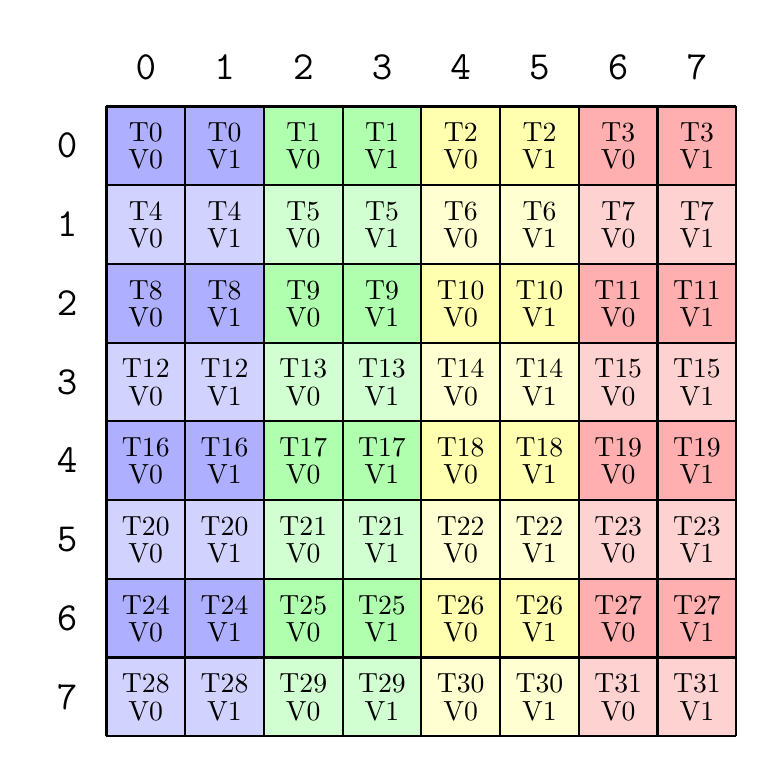
\begin{tikzpicture}[x={(0cm,-1cm)},y={(1cm,0cm)},every node/.style={minimum size=1cm, outer sep=0pt}]
\node[fill={rgb,255:red,175;green,175;blue,255}] at (0,0) {\shortstack{T0 \\ V0}};
\node[fill={rgb,255:red,175;green,175;blue,255}] at (0,1) {\shortstack{T0 \\ V1}};
\node[fill={rgb,255:red,175;green,255;blue,175}] at (0,2) {\shortstack{T1 \\ V0}};
\node[fill={rgb,255:red,175;green,255;blue,175}] at (0,3) {\shortstack{T1 \\ V1}};
\node[fill={rgb,255:red,255;green,255;blue,175}] at (0,4) {\shortstack{T2 \\ V0}};
\node[fill={rgb,255:red,255;green,255;blue,175}] at (0,5) {\shortstack{T2 \\ V1}};
\node[fill={rgb,255:red,255;green,175;blue,175}] at (0,6) {\shortstack{T3 \\ V0}};
\node[fill={rgb,255:red,255;green,175;blue,175}] at (0,7) {\shortstack{T3 \\ V1}};
\node[fill={rgb,255:red,210;green,210;blue,255}] at (1,0) {\shortstack{T4 \\ V0}};
\node[fill={rgb,255:red,210;green,210;blue,255}] at (1,1) {\shortstack{T4 \\ V1}};
\node[fill={rgb,255:red,210;green,255;blue,210}] at (1,2) {\shortstack{T5 \\ V0}};
\node[fill={rgb,255:red,210;green,255;blue,210}] at (1,3) {\shortstack{T5 \\ V1}};
\node[fill={rgb,255:red,255;green,255;blue,210}] at (1,4) {\shortstack{T6 \\ V0}};
\node[fill={rgb,255:red,255;green,255;blue,210}] at (1,5) {\shortstack{T6 \\ V1}};
\node[fill={rgb,255:red,255;green,210;blue,210}] at (1,6) {\shortstack{T7 \\ V0}};
\node[fill={rgb,255:red,255;green,210;blue,210}] at (1,7) {\shortstack{T7 \\ V1}};
\node[fill={rgb,255:red,175;green,175;blue,255}] at (2,0) {\shortstack{T8 \\ V0}};
\node[fill={rgb,255:red,175;green,175;blue,255}] at (2,1) {\shortstack{T8 \\ V1}};
\node[fill={rgb,255:red,175;green,255;blue,175}] at (2,2) {\shortstack{T9 \\ V0}};
\node[fill={rgb,255:red,175;green,255;blue,175}] at (2,3) {\shortstack{T9 \\ V1}};
\node[fill={rgb,255:red,255;green,255;blue,175}] at (2,4) {\shortstack{T10 \\ V0}};
\node[fill={rgb,255:red,255;green,255;blue,175}] at (2,5) {\shortstack{T10 \\ V1}};
\node[fill={rgb,255:red,255;green,175;blue,175}] at (2,6) {\shortstack{T11 \\ V0}};
\node[fill={rgb,255:red,255;green,175;blue,175}] at (2,7) {\shortstack{T11 \\ V1}};
\node[fill={rgb,255:red,210;green,210;blue,255}] at (3,0) {\shortstack{T12 \\ V0}};
\node[fill={rgb,255:red,210;green,210;blue,255}] at (3,1) {\shortstack{T12 \\ V1}};
\node[fill={rgb,255:red,210;green,255;blue,210}] at (3,2) {\shortstack{T13 \\ V0}};
\node[fill={rgb,255:red,210;green,255;blue,210}] at (3,3) {\shortstack{T13 \\ V1}};
\node[fill={rgb,255:red,255;green,255;blue,210}] at (3,4) {\shortstack{T14 \\ V0}};
\node[fill={rgb,255:red,255;green,255;blue,210}] at (3,5) {\shortstack{T14 \\ V1}};
\node[fill={rgb,255:red,255;green,210;blue,210}] at (3,6) {\shortstack{T15 \\ V0}};
\node[fill={rgb,255:red,255;green,210;blue,210}] at (3,7) {\shortstack{T15 \\ V1}};
\node[fill={rgb,255:red,175;green,175;blue,255}] at (4,0) {\shortstack{T16 \\ V0}};
\node[fill={rgb,255:red,175;green,175;blue,255}] at (4,1) {\shortstack{T16 \\ V1}};
\node[fill={rgb,255:red,175;green,255;blue,175}] at (4,2) {\shortstack{T17 \\ V0}};
\node[fill={rgb,255:red,175;green,255;blue,175}] at (4,3) {\shortstack{T17 \\ V1}};
\node[fill={rgb,255:red,255;green,255;blue,175}] at (4,4) {\shortstack{T18 \\ V0}};
\node[fill={rgb,255:red,255;green,255;blue,175}] at (4,5) {\shortstack{T18 \\ V1}};
\node[fill={rgb,255:red,255;green,175;blue,175}] at (4,6) {\shortstack{T19 \\ V0}};
\node[fill={rgb,255:red,255;green,175;blue,175}] at (4,7) {\shortstack{T19 \\ V1}};
\node[fill={rgb,255:red,210;green,210;blue,255}] at (5,0) {\shortstack{T20 \\ V0}};
\node[fill={rgb,255:red,210;green,210;blue,255}] at (5,1) {\shortstack{T20 \\ V1}};
\node[fill={rgb,255:red,210;green,255;blue,210}] at (5,2) {\shortstack{T21 \\ V0}};
\node[fill={rgb,255:red,210;green,255;blue,210}] at (5,3) {\shortstack{T21 \\ V1}};
\node[fill={rgb,255:red,255;green,255;blue,210}] at (5,4) {\shortstack{T22 \\ V0}};
\node[fill={rgb,255:red,255;green,255;blue,210}] at (5,5) {\shortstack{T22 \\ V1}};
\node[fill={rgb,255:red,255;green,210;blue,210}] at (5,6) {\shortstack{T23 \\ V0}};
\node[fill={rgb,255:red,255;green,210;blue,210}] at (5,7) {\shortstack{T23 \\ V1}};
\node[fill={rgb,255:red,175;green,175;blue,255}] at (6,0) {\shortstack{T24 \\ V0}};
\node[fill={rgb,255:red,175;green,175;blue,255}] at (6,1) {\shortstack{T24 \\ V1}};
\node[fill={rgb,255:red,175;green,255;blue,175}] at (6,2) {\shortstack{T25 \\ V0}};
\node[fill={rgb,255:red,175;green,255;blue,175}] at (6,3) {\shortstack{T25 \\ V1}};
\node[fill={rgb,255:red,255;green,255;blue,175}] at (6,4) {\shortstack{T26 \\ V0}};
\node[fill={rgb,255:red,255;green,255;blue,175}] at (6,5) {\shortstack{T26 \\ V1}};
\node[fill={rgb,255:red,255;green,175;blue,175}] at (6,6) {\shortstack{T27 \\ V0}};
\node[fill={rgb,255:red,255;green,175;blue,175}] at (6,7) {\shortstack{T27 \\ V1}};
\node[fill={rgb,255:red,210;green,210;blue,255}] at (7,0) {\shortstack{T28 \\ V0}};
\node[fill={rgb,255:red,210;green,210;blue,255}] at (7,1) {\shortstack{T28 \\ V1}};
\node[fill={rgb,255:red,210;green,255;blue,210}] at (7,2) {\shortstack{T29 \\ V0}};
\node[fill={rgb,255:red,210;green,255;blue,210}] at (7,3) {\shortstack{T29 \\ V1}};
\node[fill={rgb,255:red,255;green,255;blue,210}] at (7,4) {\shortstack{T30 \\ V0}};
\node[fill={rgb,255:red,255;green,255;blue,210}] at (7,5) {\shortstack{T30 \\ V1}};
\node[fill={rgb,255:red,255;green,210;blue,210}] at (7,6) {\shortstack{T31 \\ V0}};
\node[fill={rgb,255:red,255;green,210;blue,210}] at (7,7) {\shortstack{T31 \\ V1}};
\draw[color=black,thick,shift={(-0.5,-0.5)}] (0,0) grid (8,8);
\node at (0,-1) {\Large{\texttt{0}}};
\node at (1,-1) {\Large{\texttt{1}}};
\node at (2,-1) {\Large{\texttt{2}}};
\node at (3,-1) {\Large{\texttt{3}}};
\node at (4,-1) {\Large{\texttt{4}}};
\node at (5,-1) {\Large{\texttt{5}}};
\node at (6,-1) {\Large{\texttt{6}}};
\node at (7,-1) {\Large{\texttt{7}}};
\node at (-1,0) {\Large{\texttt{0}}};
\node at (-1,1) {\Large{\texttt{1}}};
\node at (-1,2) {\Large{\texttt{2}}};
\node at (-1,3) {\Large{\texttt{3}}};
\node at (-1,4) {\Large{\texttt{4}}};
\node at (-1,5) {\Large{\texttt{5}}};
\node at (-1,6) {\Large{\texttt{6}}};
\node at (-1,7) {\Large{\texttt{7}}};
\end{tikzpicture}
}
\caption{Ampere FP64 Tensor Core 所要求的 $8 {\times} 8$ C 矩阵的线程-值划分。}
\label{fig:TVLayout}
\end{figure}

考察一个细化了形状 $(8,8)$ 的数据布局。我们的目标是使用图~\ref{fig:TVLayout} 所示的线程-值模式对该数据进行划分，该模式是某个特定 Ampere Tensor Core 的逻辑划分模式。这条指令的线程-值划分模式可以用布局
\begin{align*}
\texttt{ThrValLayoutC:} \quad ((4,8),2):((16,1),8),
\end{align*}
表示，它充当从 $(\texttt{thread\_idx}, \texttt{value\_idx})$ 到 $8 {\times} 8$ 矩阵内一维坐标的映射。如图所示，出于人类可读性的考虑，图~\ref{fig:TVLayout} 实际上画出的是其逆——它展示的是从 $8 {\times} 8$ 矩阵内的二维坐标到 $(\texttt{thread\_idx}, \texttt{value\_idx})$ 二元组的映射。这个 {\tt ThrValLayoutC} 被视为 Ampere Tensor Core 指令的静态元数据——它是指令与硬件功能的内在属性；在 \CuTe 出现之前，它只能以指令集架构（ISA）中类似图~\ref{fig:TVLayout} 的图像来描述。

任意 $8 {\times} 8$ 数据布局都可以通过与线程-值布局 {\tt ThrValLayoutC} 复合而被置换。每次复合都会产生一个与形状 $(32,2)$ 相容的布局，并定义 $(\texttt{thread\_idx}, \texttt{value\_idx})$ 与数据偏移之间的映射。例如，表~\ref{tab:TVLayoutExamples} 展示了若干数据布局经上述 {\tt ThrValLayoutC} 复合变换的例子。

\begin{table}[ht]
\centering
\begin{tabular}{|c|c|c|c|}
数据名称 & 数据布局 $8 {\times} 8$（$\v{A}$） & 线程-值布局 $32 {\times} 2$（$\v{B}$） & 结果 $32 {\times} 2$（$\v{R}$） \\ \hline \hline
{\tt ColMajor} & $(8,8):(1,8)$ & $((4,8),2):((16,1),8)$ & $((4,8),2):((16,1),8)$ \\ \hline
{\tt RowMajor} & $(8,8):(8,1)$ & $((4,8),2):((16,1),8)$ & $((4,8),2):((2,8),1)$ \\ \hline
{\tt Padded} & $(8,8):(1,9)$ & $((4,8),2):((16,1),8)$ & $((4,8),2):((18,1),9)$ \\ \hline
{\tt ColInterleaved} & $((4,2),(2,4)):((2,16),(1,8))$ & $((4,8),2):((16,1),8)$ & $((4,(4,2)),2):((8,(2,16)),1)$ \\ \hline
{\tt Swizzled} & $(8,8):(f_1,f_9)$ & $((4,8),2):((16,1),8)$ & $((4,8),2):((f_{18},f_1),f_9)$ \\ \hline
{\tt Coordinate} & $(8,8):(e_0,e_1)$ & $((4,8),2):((16,1),8)$ & $((4,8),2):((2e_1,e_0),e_1)$ \\ \hline
\end{tabular}
\caption{数据布局经线程-值（TV）布局复合变换的示例。}
\label{tab:TVLayoutExamples}
\end{table}

下面的代码展示了一种使用线程-值划分的常见模式：
\begin{python}
smem_data = Tensor(MyAccessor, MyLayout8x8)     # Tensor：Coord -> Offset
tv_layout   = Layout(((4,8),2), ((16,1),8))     # TV 布局：(Thr,Val) -> Coord
smem_tv     = composition(smem_data, tv_layout) # 复合：(Thr,Val) -> Offset
smem_v      = smem_tv[thr_id, None]             # 按线程切片得到子张量
copy(smem_v, rmem_data)                         # 拷贝到寄存器张量/数组
\end{python}
这一模式在 SIMD 编程中极为常见：每个处理元素接收某个父数据的一个对称划分。一般而言，\CuTe 认识到任意划分都可以定义为复合（置换和/或重塑形）之后再切片。如第~\ref{sec:slicing} 节所述，这种“复合-切片”模式把划分模式（{\tt ThrValLayoutC}）与实际切出的数据切片（以 {\tt thr\_id} 做的切片）分离开来。由于划分模式往往是指令或优化参数相关的编译期元数据，而切片往往是运行时的程序标识索引，这一模式更有能力传播静态信息并降低运行时开销。

\wpssh{逐模复合与分块器（By-mode Composition and Tilers）}
\label{sec:tiler}

群复合可以逐模应用，从而支持对布局的子定义域进行操作。例如，常常需要对矩阵的行与列独立地应用复合。我们使用式~\eqref{eqn:layout_combinator} 中的组合子，并把其中的 $\star$ 运算取为群复合 $\circ$，从而对布局的各个独立子布局分别应用复合。

我们把式~\eqref{eqn:layout_combinator} 中的布局元组称为{\em 分块器}（Tiler）。
\begin{definition}
{\em 分块器}（Tiler）是一个 $\texttt{HTuple}(\texttt{Tile})$，其中每个 \texttt{Tile} 是
\begin{compactitem}
\item 一个 \textit{Layout} $S:D$，或
\item 一个 \textit{Integer} $S$，等价地视作布局 $S:1$。
\end{compactitem}
\end{definition}
该定义意味着所有布局都是分块器，所有整数也都是分块器，并且允许 $(4,8)$ 这样的形状用作分块器。图~\ref{fig:48tile} 展示了这一常见情形：形状可以作为提取并操作子布局的便捷分块器。

\begin{figure}[ht]
\centering
\begin{subfigure}{0.22\textwidth}
\centering
\resizebox{\linewidth}{!}{
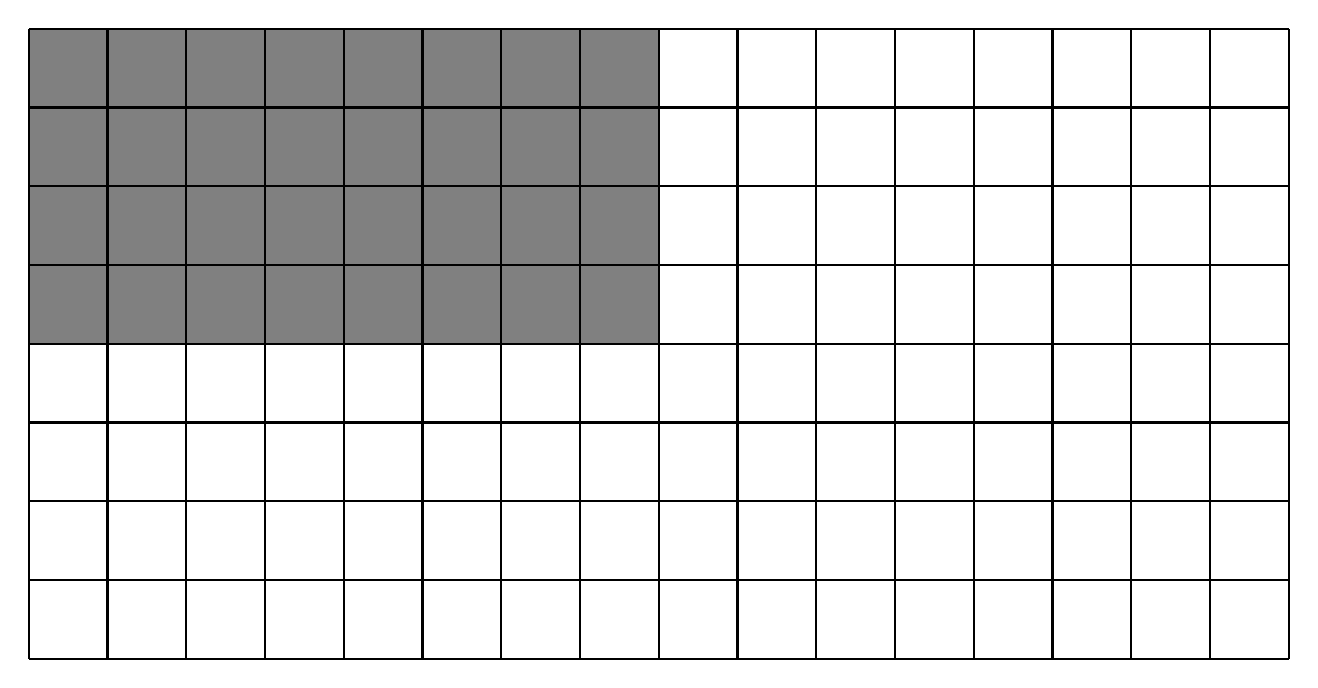
\begin{tikzpicture}[x={(0cm,-1cm)},y={(1cm,0cm)},every node/.style={minimum size=1cm, outer sep=0pt}]
\foreach \i in {0,1,2,3} {
\foreach \j in {0,1,2,3,4,5,6,7} {
\node[fill=gray] at (\i,\j) {};
}}
\draw[color=black,thick,shift={(-0.5,-0.5)}] (0,0) grid (8,16);
\end{tikzpicture}}
\caption{$\langle 4:1,8:1 \rangle \equiv \langle 4,8 \rangle$}
\label{fig:48tile}
\end{subfigure}\quad
\begin{subfigure}{0.22\textwidth}
\centering
\resizebox{\linewidth}{!}{
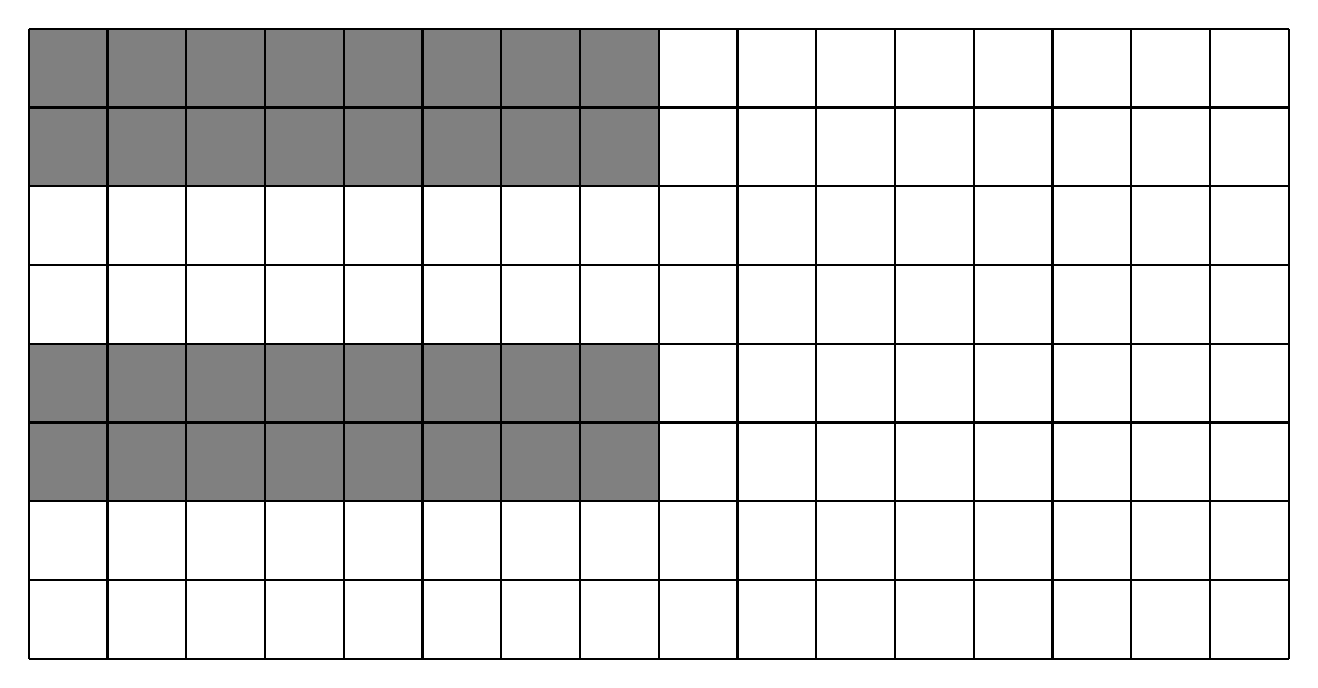
\begin{tikzpicture}[x={(0cm,-1cm)},y={(1cm,0cm)},every node/.style={minimum size=1cm, outer sep=0pt}]
\foreach \i in {0,1,4,5} {
\foreach \j in {0,1,2,3,4,5,6,7} {
\node[fill=gray] at (\i,\j) {};
}}
\draw[color=black,thick,shift={(-0.5,-0.5)}] (0,0) grid (8,16);
\end{tikzpicture}}
\caption{$\langle (2,2):(1,4),8:1 \rangle$}
\end{subfigure}\quad
\begin{subfigure}{0.22\textwidth}
\centering
\resizebox{\linewidth}{!}{
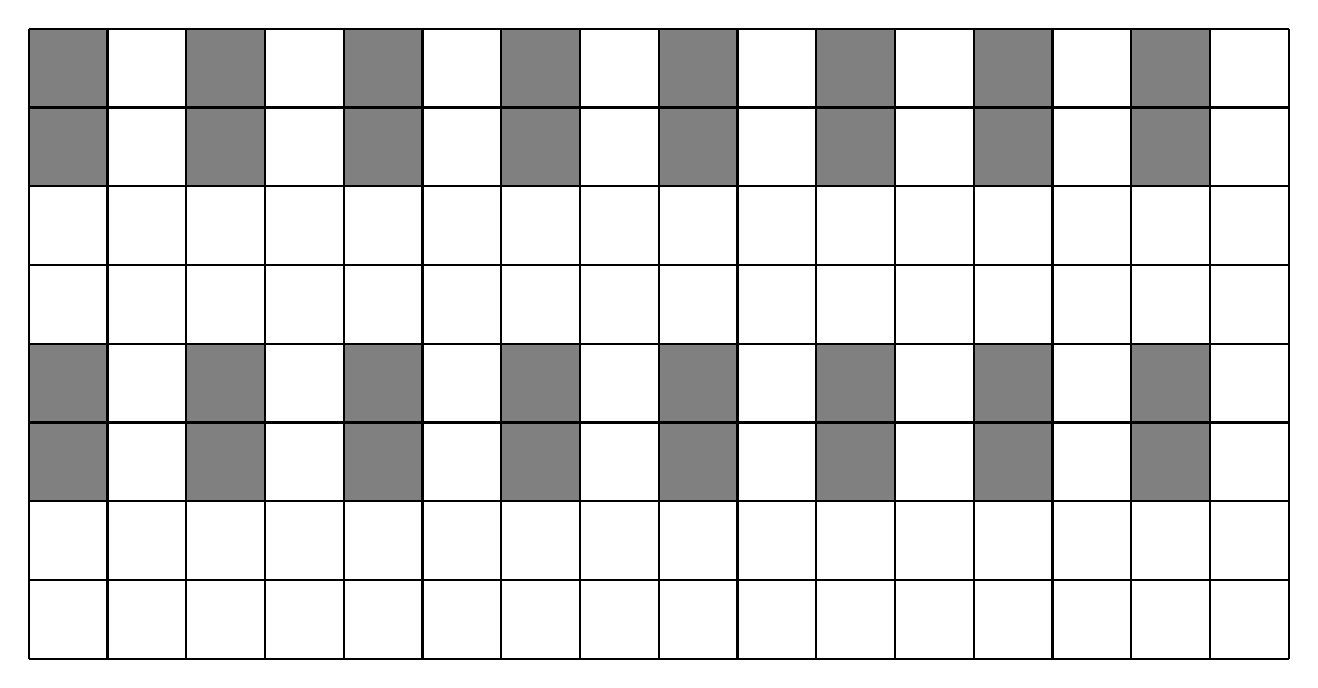
\begin{tikzpicture}[x={(0cm,-1cm)},y={(1cm,0cm)},every node/.style={minimum size=1cm, outer sep=0pt}]
\foreach \i in {0,1,4,5} {
\foreach \j in {0,2,4,6,8,10,12,14} {
\node[fill=gray] at (\i,\j) {};
}}
\draw[color=black,thick,shift={(-0.5,-0.5)}] (0,0) grid (8,16);
\end{tikzpicture}}
\caption{$\langle (2,2):(1,4),8:2 \rangle$}
\end{subfigure}\quad
\begin{subfigure}{0.22\textwidth}
\centering
\resizebox{\linewidth}{!}{
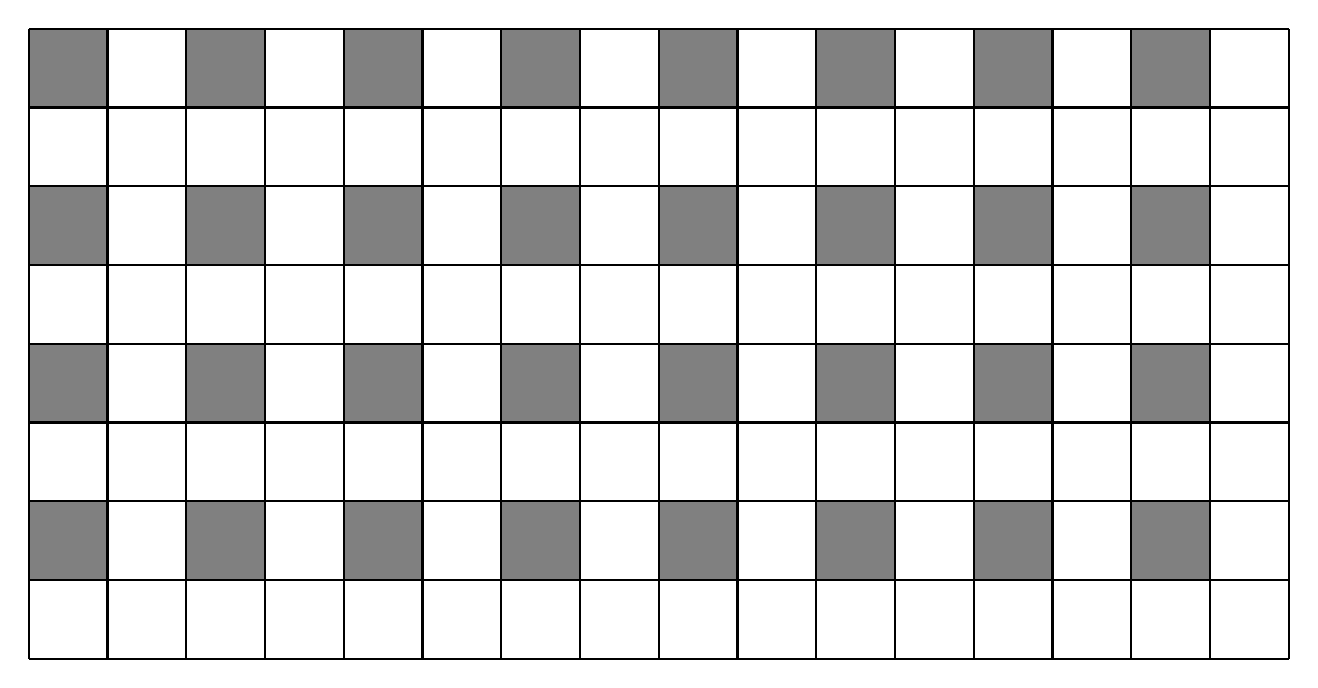
\begin{tikzpicture}[x={(0cm,-1cm)},y={(1cm,0cm)},every node/.style={minimum size=1cm, outer sep=0pt}]
\foreach \i in {0,2,4,6} {
\foreach \j in {0,2,4,6,8,10,12,14} {
\node[fill=gray] at (\i,\j) {};
}}
\draw[color=black,thick,shift={(-0.5,-0.5)}] (0,0) grid (8,16);
\end{tikzpicture}}
\caption{$\langle 4:2,8:2 \rangle$}
\end{subfigure}
\caption{通过 $\v{L} \circ \v{T}$ 从任意 $8{\times}16$ 布局 $\v{L}$ 中提取 $4 {\times} 8$ 子布局的分块器 $\v{T}$ 示例。}
\label{fig:tilers}
\end{figure}

图~\ref{fig:tilers} 展示了分块器如何通过复合作用于任意布局。图中取一个与形状 $(8,16)$ 相容的任意布局，并应用各种分块器分别从列和行中提取元素，从而产生与形状 $(4,8)$ 相容的子布局。例如，分块器 $\langle 4:1, 8:1 \rangle$ 从每列提取前 4 个元素、从每行提取前 8 个元素，产生与形状 $(4,8)$ 相容的子布局。

此外，分块器的复合与坐标布局的复合之间存在等价关系。对布局 $\v{L} = (M,N) : (X,Y)$ 与分块器 $\v{T} = \langle \v{T}_0, \v{T}_1 \rangle$，我们注意到
\begin{align*}
\v{L} \ \circ \ \v{T} \ \equiv \ \v{L} \ \circ \ (M,N):(e_0,e_1) \ \circ \ \v{T}
\end{align*}
这意味着 $(M,N):(e_0,e_1) \ \circ \ \v{T}$ 对 $\v{L}$ 的作用与 $\v{T}$ 的作用相同。这里 $(M,N):(e_0,e_1)$ 是一个恒等布局，把二维自然坐标映射到二维坐标。分块器的这种表述巩固了如下观念：形状可以被视为从坐标到自然坐标的映射，正如第~\ref{sec:layout} 节中 Layout 的定义所采用的那样。具体而言，在复合中以下对象应视为等价：
\begin{align*}
(4,8) \equiv \langle 4, 8 \rangle \equiv (4:1, 8:1) \equiv (4,8):(e_0,e_1)
\end{align*}

%% wp6 逆布局：右逆、左逆及应用（论文 Inverse 小节）
\wpsh{逆（Inverse）}
\label{sec:inverse}

布局可以是单射（injective）、满射（surjective）或双射（bijective）的，并且存在右逆（right-inverse）、左逆（left-inverse）、全逆（full-inverse）与拟逆（quasi-inverse）。当把布局解释为从坐标到偏移的函数时，逆布局便可解释为从偏移到坐标的函数。布局的逆很有用：确定某些偏移在布局中的位置、提取由特定偏移构成的组，或确定两个布局各自的公共子布局。

本节定义布局的广义左逆与右逆，并给出使用它们的应用示例。

\wpssh{右逆（Right-Inverse）}

布局 $\v{L} : \Z_{\abs{\v{L}}} \to \D$ 的{\em 右（伪）逆}是一个单射布局 $\v{L}^{\ddagger} : \D_{\v{L}^{\ddagger}} \to \Z_{\abs{\v{L}}}$，满足
\begin{align}
\forall k \in \D_{\v{L}^{\ddagger}}, \ \ \v{L}^\ddagger(\v{L}(\v{L}^\ddagger(k))) &= \v{L}^\ddagger(k)
\label{eqn:right-inverse}
\end{align}
当 $\v{L}$ 具有一般的整数半模（integer-semimodule）陪域（codomain）$\D$ 时，上述一般性定义可用来刻画 $\v{L}^{\ddagger}$ 的性质。在常见情形 $\D = \Z$ 下，可以恢复出右逆的经典定义，
\begin{align*}
\forall k \in \Z_{\abs{\v{L}^{\ddagger}}}, \ \ \v{L}(\v{L}^{\ddagger}(k)) = k,
\end{align*}
而对于更一般的陪域，例如 $\D = \Z^{(\ast,\ast)}$，由式~\eqref{eqn:right-inverse} 可以推出 $\D \lesssim \v{L}^\ddagger$：右逆的定义域（domain）对 $\v{L}$ 陪域的轮廓做了粗化，使其能够接受来自 $\v{L}$ 的偏移。

若布局 $\v{L}$ 存在右逆布局 $\v{L}^\ddagger$，则 $\abs{\v{L}^\ddagger} \leq \abs{\v{L}}$。实践中，提到某布局的右逆时，我们通常指尺寸最大的那个右逆。例如，图~\ref{fig:layouts} 与图~\ref{fig:layouts2} 中布局的最大尺寸右逆如表~\ref{tab:rinv} 所示。

\begin{table}[ht]
\begin{center}
\begin{tabular}{|>{$}c<{$}|>{$}c<{$}|c|}
\v{L} & \v{L}^\ddagger & \textbf{备注} \\ \hline \hline
(4,8):(1,4) & 32:1 & \\ \hline
(4,8):(8,1) & (8,4):(4,1) \\ \hline
(3,7,5):(5,15,1) & (5,21):(21,1) & 非 2 的幂的形状/步幅也没有问题。 \\ \hline
(4,8):(1,5) & 4:1 & 对非连续的像，结果更小。 \\ \hline
(4,(4,2)):(4,(1,16)) & (4,4,2):(4,1,16) & 结果定义域与陪域 $\Z$ 同余。 \\ \hline
((2,2),(4,2)):((1,8),(2,16)) & (2,4,2,2):(1,4,2,16) \\ \hline
((2,2),(2,4)):((0,1),(0,2)) & (2,4):(2,8) & 步幅为 0 的模没有贡献。 \\ \hline
((2,2),(2,4)):((0,2),(0,4)) & 1:0 & 平凡右逆。 \\ \hline
(4,8):(e_0,e_1) & (4,8):(1,4) & 结果定义域与陪域 $\Z^{(\ast,\ast)}$ 同余。 \\ \hline
(4,(4,2)):(e_1,(e_0,6e_1)) & (4,4):(4,1) & 结果更小且定义域相容。 \\ \hline
(4,(4,3)):(f_1,(f_5,f_{16})) & (4,4,3):(f_1,f_5,f_{16}) & 对整数模步幅也可定义。 \\ \hline
\end{tabular}
\end{center}
\caption{布局右逆的示例。}
\label{tab:rinv}
\end{table}

当布局 $\v{L}$ 是 $\Z_{\abs{\v{L}}}$ 上的双射时，右逆同时也是布局 $\v{L}$ 的{\em 逆} $\v{L}^{-1}$，满足
\begin{align*}
\forall k \in \Z_{\abs{\v{L}}}, \ \ \v{L}(\v{L}^{-1}(k)) = k = \v{L}^{-1}(\v{L}(k))
\end{align*}
若布局 $\v{L}$ 存在全逆 $\v{L}^{-1}$，则称该布局是{\em 紧凑}（compact）的。

\wpssh{应用：向量化（Vectorization）示例}

\begin{figure}[ht]
	\centering
	\begin{subfigure}[t]{0.35\textwidth}
		\centering
		\begin{tikzpicture}[thick,scale=1.10, every node/.style={scale=1.10}]
			\begin{scope}[xshift=-1.5cm]
			\matrix[matrix of nodes,nodes={draw,inner sep=0pt,text width=.5cm,align=center,minimum height=.5cm}]
			at (0,0) {
				0 & 4 & 8  & 12 \\
				1 & 5 & 9  & 13 \\
				2 & 6 & 10 & 14 \\
				3 & 7 & 11 & 15 \\};
			\fill [gray,fill opacity=0.4] (-1.05,0) rectangle (-0.50,1.05);
			\draw (0,-1) node[anchor=north,align=center] {\footnotesize $(4,4):(1,4)$ \\ \footnotesize 源};
			\end{scope}
			\begin{scope}[xshift=+1.5cm]
			\matrix[matrix of nodes,nodes={draw,inner sep=0pt,text width=.5cm,align=center,minimum height=.5cm}]
			at (0,0) {
				0 & 2 & 4  & 6 \\
				1 & 3 & 5  & 7 \\
				8 & 10 & 12 & 14 \\
				9 & 11 & 13 & 15 \\};
			\fill [gray,fill opacity=0.4] (-1.05,0) rectangle (-0.50,1.05);
			\draw (0,-1) node[anchor=north,align=center] {\footnotesize $((2,2),4):((1,8),2)$ \\ \footnotesize 目标};
		    \end{scope}
		\end{tikzpicture}
		\caption{2 元素公共子向量。} \label{fig:autovec1}
	\end{subfigure}
    \quad\quad\quad\quad\quad\quad
	\begin{subfigure}[t]{0.5\textwidth}
	\centering
	\begin{tikzpicture}[thick,scale=1.10, every node/.style={scale=1.10}]
		\begin{scope}[xshift=-2cm]
		\matrix[matrix of nodes,nodes={draw,inner sep=0pt,text width=.5cm,align=center,minimum height=.5cm}]
		at (0,0) {
			0  & 4  & 1  & 5  \\
			8  & 12 & 9  & 13 \\
			2  & 6  & 3  & 7  \\
			10 & 14 & 11 & 15 \\};
		\fill [gray,fill opacity=0.4] (-1.05,+0.50) rectangle (-0.50,1.05);
		\fill [gray,fill opacity=0.4] (-1.05,-0.50) rectangle (-0.50,0.00);
		\fill [gray,fill opacity=0.4] (    0,+0.50) rectangle (+0.50,1.05);
		\fill [gray,fill opacity=0.4] (    0,-0.50) rectangle (+0.50,0.00);
		\draw (0,-1) node[anchor=north,align=center] {\footnotesize$((2,2),(2,2)):((8,2),(4,1))$ \\ \footnotesize 源};
		\end{scope}
		\begin{scope}[xshift=+2cm]
		\matrix[matrix of nodes,nodes={draw,inner sep=0pt,text width=.5cm,align=center,minimum height=.5cm}]
		at (0,0) {
			0 & 8 & 1  & 9 \\
			4 & 12 & 5  & 13 \\
			2 & 10 & 3 & 11 \\
			6 & 14 & 7 & 15 \\};
		\fill [gray,fill opacity=0.4] (-1.05,+0.50) rectangle (-0.50,1.05);
		\fill [gray,fill opacity=0.4] (-1.05,-0.50) rectangle (-0.50,0.00);
		\fill [gray,fill opacity=0.4] (    0,+0.50) rectangle (+0.50,1.05);
		\fill [gray,fill opacity=0.4] (    0,-0.50) rectangle (+0.50,0.00);
		\draw (0,-1) node[anchor=north,align=center] {\footnotesize $((2,2),(2,2)):((4,2),(8,1))$ \\ \footnotesize 目标};
		\end{scope}
	\end{tikzpicture}
	\caption{4 元素公共子向量。} \label{fig:autovec2}
\end{subfigure}
\caption{布局之间公共子向量的示例。}
\label{fig:autovec}
\end{figure}

判断数据布局里有没有连续元素、在什么位置，右逆非常有用。举个直接的例子：布局 $(4,8):(1,4)$ 与 $(4,8):(8,1)$ 的右逆分别是 $32:1$ 与 $(8,4):(4,1)$。两个右逆的尺寸都是 32，说明两个布局都索引 32 个连续的物理元素。

再看一个复杂些的例子：\CuTe{} 中一种常见的拷贝模式，向量化拷贝（vectorizing-copy），它要找出两个张量之间一次最多能拷贝的元素个数。右逆使 \CuTe{} 确定两个布局之间的{\em 最大公共子布局}（maximum common sublayout）；再结合硬件能力以及指针与步幅物理对齐的信息，就能以代数方式确定可安全向量化的元素数量及其位置，照此完成拷贝。

图~\ref{fig:autovec} 给出了两个向量化示例。在第一幅图~\ref{fig:autovec1} 中，源布局与目标布局在元素偏移 $k \in \{0,1\}$（对应坐标 $\bar{c} \in \{0,1\}$）处坐标一致。只要访问器（accessor）、数据类型与对齐允许，拷贝宽度即可扩展为每条指令搬运两个元素。在第二幅图~\ref{fig:autovec2} 中，源布局与目标布局在元素偏移 $k \in \{0,1,2,3\}$（对应坐标 $\bar{c} = \{0,2,8,10\}$）处坐标一致，拷贝宽度可扩展为每条指令搬运四个元素。

一般地，对满足 $\abs{\v{A}} = \abs{\v{B}}$ 的布局 $\v{A} : \Z(\v{A}) \to \Z_\alpha$ 与 $\v{B} : \Z(\v{B}) \to \Z_\beta$，我们希望找到最大的整数 $K$，使得坐标相匹配
\begin{align*}
\forall \, k \in \Z_K, \ \ \v{A}^\ddagger(k) = \v{B}^\ddagger(k)
\end{align*}
并且这一最大值可以通过寻找满足下式的 $K$ 来高效计算：
\begin{align*}
\forall \, k \in \Z_K, \ \ k = \v{A}(\v{B}^\ddagger(k)) = (\v{A} \circ \v{B}^\ddagger)(k) \quad \text{或} \quad
\forall \, k \in \Z_K, \ \ k = \v{B}(\v{A}^\ddagger(k)) = (\v{B} \circ \v{A}^\ddagger)(k)
\end{align*}
也就是 $\v{A} \circ \v{B}^\ddagger = (\v{I}_K, \v{X})$ 或 $\v{B} \circ \v{A}^\ddagger = (\v{I}_K, \v{Y})$ 中恒等部分（步幅为 1 的模）的尺寸。

这些相互连续的元素，其整数坐标由下式给出
\begin{align}
\v{A}^\ddagger \circ  \floor{\v{B} \circ \v{A}^\ddagger}_K = \v{A}^\ddagger \circ \v{I}_K = \floor{\v{A}^\ddagger}_K  \ \colon \ \Z_K \to \Z_{\abs{A}} \nonumber \\
\v{B}^\ddagger \circ  \floor{\v{A} \circ \v{B}^\ddagger}_K = \v{B}^\ddagger \circ \v{I}_K = \floor{\v{B}^\ddagger}_K  \ \colon \ \Z_K \to \Z_{\abs{B}}
\label{eqn:common_layout}
\end{align}
其中 $\floor{\cdot}_K$ 是在尺寸 $K$ 处截断的操作。该布局给出数据中前 $K$ 个物理元素的逻辑坐标，并可通过 \texttt{logical\_divide} 或 \texttt{zipped\_divide}（第~\ref{sec:logical_divide} 节）从中提取出公共子向量。

在实践中，考虑第~\ref{sec:copy} 节中的参考函数 {\tt COPY}。该实现可以在不改变可观察行为的前提下，在内部置换迭代顺序。置换迭代顺序等价于对源张量与目标张量的布局施加同一个一致的置换。选取与式~\eqref{eqn:common_layout} 所定义布局相匹配的置换，所有连续元素都会被换到第一个模中，由向量化指令做特殊处理。这一过程既能检测待向量化的元素是否存在及其位置，也能确定可安全向量化的最大元素数；{\bf 自动向量化}（AutoVectorization）就建立在这套流程之上。

\wpssh{左逆（Left-Inverse）}

布局 $\v{L} : \Z_{\abs{\v{L}}} \to \D$ 的{\em 左（伪）逆}是一个布局 $\v{L}^{\dagger} : \D_{\v{L}^\dagger} \to \Z_{\abs{\v{L}}}$，满足
\begin{align}
\forall k \in \Z_{\abs{\v{L}}}, \ \ \v{L}(\v{L}^{\dagger}(\v{L}(k))) = \v{L}(k)
\end{align}
左逆可能不唯一，并且对于不在 $\v{L}$ 的像（image）中的输入，左逆可以取任意值。当 $\v{L}$ 具有一般的整数半模陪域 $\D$ 时，上述一般性定义同样可用来刻画 $\v{L}^{\dagger}$ 的性质。在 $\v{L}$ 为单射这一常见情形下，可以恢复出左逆的经典定义，
\begin{align*}
\forall k \in \Z_{\abs{\v{L}}}, \ \ \v{L}^\dagger(\v{L}(k)) = k.
\end{align*}

图~\ref{fig:layouts} 与图~\ref{fig:layouts2} 中布局的左逆如表~\ref{tab:linv} 所示。

\begin{table}[ht]
\begin{center}
\begin{tabular}{|>{$}c<{$}|>{$}c<{$}|c|}
\v{L} & \v{L}^\dagger & 备注 \\ \hline \hline
(4,8):(1,4) & 32:1 \\ \hline
(4,8):(8,1) & (8,4):(4,1) & 对连续的像，与右逆相同。 \\ \hline
(3,7,5):(5,15,1) & (5,21):(21,1) & 非 2 的幂的形状/步幅也没有问题。 \\ \hline
(4,8):(1,5) & (5,8):(1,4) & 对非连续的像，结果更大。 \\ \hline
(4,(4,2)):(4,(1,16)) & (4,4,2):(4,1,16) & 结果定义域与陪域 $\Z$ 同余。 \\ \hline
((2,2),(4,2)):((1,8),(2,16)) & (2,4,2,2):(1,4,2,16) \\ \hline
((2,2),(2,4)):((0,2),(0,4)) & (2,2,4):(0,2,8) & 结果不唯一——模 0 的步幅可任取。 \\ \hline
((2,2),(2,4)):((0,1),(0,2)) & (2,4):(2,8) \\ \hline
(4,8):(e_0,e_1) & (4,8):(1,4) & 结果定义域与陪域 $\Z^{(\ast,\ast)}$ 同余。 \\ \hline
(4,(4,2)):(e_1,(e_0,6e_1)) & (4,(6,2)):(4,(1,16)) & 结果更大且定义域相容。 \\ \hline
(4,(4,3)):(f_1,(f_5,f_{16})) & (4,4,3):(f_1,f_5,f_{16}) & 对整数模步幅也可定义。 \\ \hline
\end{tabular}
\end{center}
\caption{布局左逆的示例。}
\label{tab:linv}
\end{table}

\wpssh{应用：容许性（Admissibility）示例}

左逆用来确定某个数据布局所产生的特定偏移是否存在及其所在位置。

\begin{figure}[ht]
\centering
\begin{subfigure}[b]{0.45\textwidth}
    \centering
    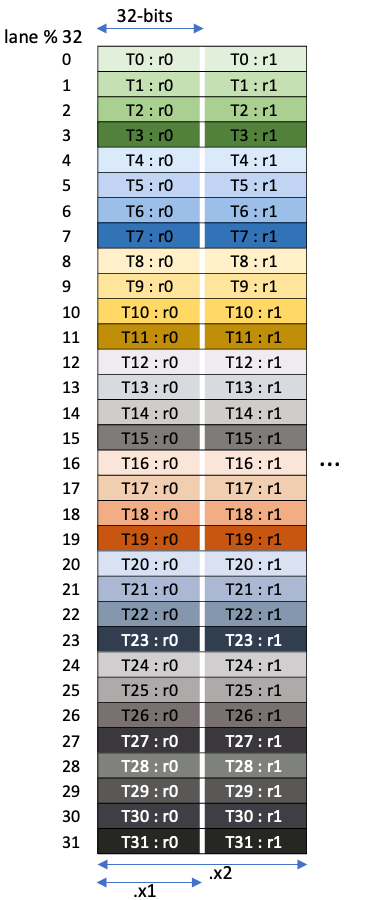
\includegraphics[width=0.3\textwidth]{figures/tikz/wp-tcgen05-tmem-fragment-3232b.png}
    \caption{\texttt{tcgen05\{.ld,.st\}.32x32b.\{x1,x2\}}}
    \label{fig:tmem_fragment-32x32}
\end{subfigure}
\hfill
\begin{subfigure}[b]{0.45\textwidth}
    \centering
    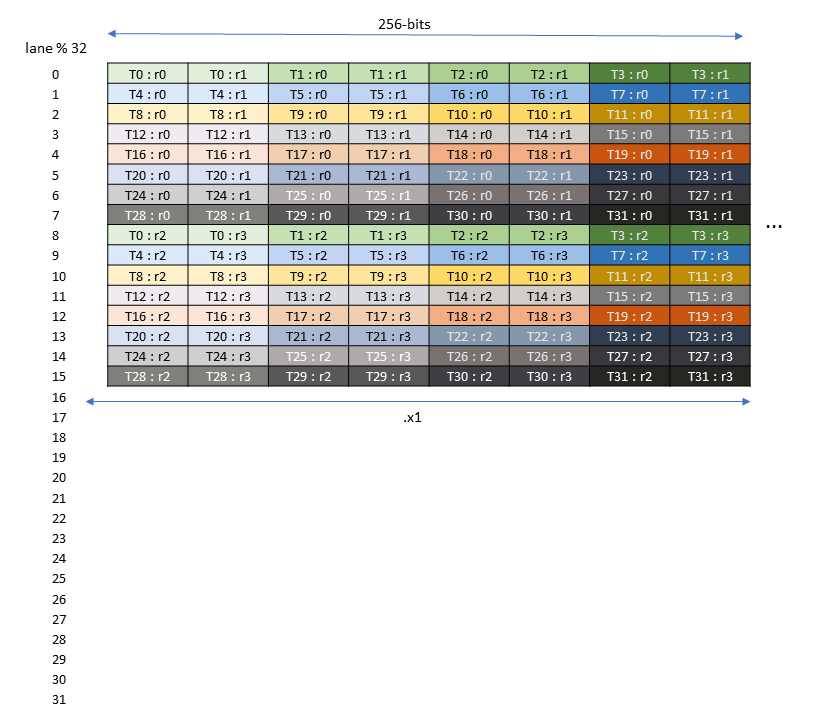
\includegraphics[width=0.8\textwidth]{figures/tikz/wp-tcgen05-tmem-fragment-16256b.png}
    \caption{\texttt{tcgen05\{.ld,.st\}.16x256b.x1}}
    \label{fig:tmem-fragment-16x256}
\end{subfigure}
\caption{TMEM load/store 指令访问特定的偏移，并将数据分配到线程本地寄存器（NVIDIA Corporation 2025）。}
\label{fig:tmem-fragments}
\end{figure}

向 Blackwell 的“张量内存”（tensor memory，TMEM）加载以及从其存储数据所使用的指令，会以一组预定义且非常特定的偏移访问 TMEM，如图~\ref{fig:tmem-fragments} 所示。物理 TMEM 的编址是一个二维网格，最多包含 512 个“列”（col）与 128 个“通道”（lane）。图中是每条指令单个 warp 的访问模式；每条指令实际使用四个 warp，上述模式每 32 个通道重复一次、共重复四次。在对物理 TMEM 编址时，沿 32 位的“列”方向跨越一步使 TMEM 地址增加 1，沿“通道”方向向下跨越一步使 TMEM 地址增加 16384。基于这一物理编址，我们定义记录每条指令所访问的全部物理偏移的布局：
\begin{center}
\begin{tabular}{l | r@{:}l}
\quad\quad\quad\quad \textbf{指令} & \multicolumn{2}{c}{$(\text{指令 COL}, \text{指令 LANE}) \to \text{TMEM 偏移}$} \\
\hline
\texttt{tcgen05\{.ld,.st\}.32x32b.x1} & $(1,128)$ & $(1,16384)$ \\
\texttt{tcgen05\{.ld,.st\}.32x32b.x2} & $(2,128)$ & $(1,16384)$ \\
\texttt{tcgen05\{.ld,.st\}.16x256b.x1} & $(8,(16,4))$ & $(1,(16384,32\cdot 16384))$ \\
\end{tabular}
\end{center}
这些布局与具体指令一一对应，可用来精确确定每条指令将访问 TMEM 中的哪些偏移。

尽管 TMEM 采用二维编址，并被用作形状为 $(M,N)$ 的 MMA 的累加器，TMEM 的“通道”与“列”并不总与逻辑矩阵的行和列相对应。与任何编址方式一样，物理偏移可以通过任意的 \CuTe{} 布局被回绕并折叠成任意形状。因此，给定一个数据布局与一条 TMEM 指令，我们希望确定
\begin{enumerate}[itemsep=0pt,topsep=2pt]
\item 数据布局是否包含该指令将访问的全部偏移；以及
\item 指令所访问的偏移在数据布局中位于何处（以逻辑坐标表示）。
\end{enumerate}

一般地，设数据布局 $\v{A} : \Z(\v{A}) \to \Z_\alpha$ 将逻辑坐标映射到数据偏移，指令布局 $\v{T} : \Z(\v{T}) \to \Z_\beta$ 将指令坐标映射到数据偏移，我们希望确定所有偏移 $\v{T}(i)$ 在 $\v{A}$ 的像中的存在性及其位置。将其表述为
\begin{align*}
\forall i \in \Z_{\abs{\v{T}}}, \exists c \in \Z(\v{A}) \ \ s.t. \ \ \v{T}(i) = \v{A}(c)
\end{align*}
该问题可以通过计算 $\v{A}$ 的左逆并检验下式来高效求解：
\begin{align*}
\v{A}(\v{A}^\dagger(\v{T}(i))) = \v{T}(i)
\end{align*}
也就是说，
\begin{compactitem}
\item 所有偏移 $\v{T}(i)$ 都在 $\v{A}^\dagger$ 的定义域中。
\item 所有坐标 $\v{A}^\dagger(\v{T}(i))$ 都互不相同，且都在 $\v{A}$ 的定义域中。
\end{compactitem}
在这些条件下，我们可以断言：每个偏移 $\v{T}(i)$ 都出现在 $\v{A}$ 的像中，且位于坐标 $\v{A}^\dagger(\v{T}(i))$ 处。布局 $\v{A}^\dagger \circ \v{T}$ 把指令坐标映射到逻辑数据坐标，例如可借助 {\tt zipped\_divide} 把数据布局 $\v{A}$ 切分为与该指令所访问偏移相对应的若干子布局。

%% wp7 补布局、逻辑乘积/逻辑切分、结论与致谢（论文收尾）
\wpsh{补}
\label{sec:complement}

布局（layout）$\v{L} : \Z(\v{L}) \to \D$ 的\emph{补}（complement）是一个满足下列条件的布局 $\v{L}^* : \Z(\v{L}^*) \to \D$
\begin{align}
\label{eqn:comp:congruence}
\text{与陪域弱同余：} && \D \lesssim \v{L}^*, \\
\label{eqn:comp:disjoint}
\text{像互不相交：} && \forall b \in \Z(\v{L}), \ \forall a \in \Z^{\v{L}^*}/\{0\}, \ &\v{L}(b) \neq \v{L}^*(a), \\
\label{eqn:comp:ordered}
\text{像有序：} && \forall a \in \Z_{\abs{\v{L}^*}}/\{0\}, \ &\v{L}^*(a-1) < \v{L}^*(a).
%\text{\emph{???:}} && \v{L}^\dagger (\v{L}, \v{L}^*) \v{L}^\dagger = \v{L}^\dagger
\end{align}
布局的补是一个在原布局的陪域（codomain）之中、但不在其像（image）之中生成元素的布局。在复合（Composition）中，布局 $\v{L}$ 常被用作对另一个布局的间接寻址，因此补 $\v{L}^*$ 就是指向 $\v{L}$ 所遗漏元素的那个布局。{\tt complement} 操作使得可以经由\emph{逻辑切分}（logical divide）（第~\ref{sec:logical_divide}~节）切分布局，并经由\emph{逻辑乘积}（logical product）（第~\ref{sec:logical_product}~节）实现布局的重复与扩展。

本节只关注陪域 $\D$ 为 {\tt HTuple}($\Z$) 的布局：即整数，或对某个轮廓 D 而言 $\D = \Z^D$ 的坐标。这使得弱同余条件式~\eqref{eqn:comp:congruence} 得以成立。像互不相交条件（式~\eqref{eqn:comp:disjoint}）保证补所生成的值与原布局生成的值互不相同。注意，这里使用的是原布局的有限定义域 $\Z(\v{L})$，而使用的是补的无穷扩展定义域 $\Z^{\v{L}^*}$。这保证了无论补的形状被截断还是被扩展（例如通过与右侧的布局复合），它所生成的值始终与原布局不同。最后，像有序条件（式~\eqref{eqn:comp:ordered}）确立了补布局的唯一性。

表~\ref{tab:complements} 给出了补的若干例子。

\begin{table}[ht]
\begin{center}
\begin{tabular}{|>{$}c<{$}|>{$}c<{$}|c|}
\v{L} & \v{L}^* & 备注 \\ \hline \hline
(4,8):(1,4) & 1:32 & 注意 $\forall i \in \Z^+, \v{L}^*(i) > \max_{j \in \Z_\v{L}} \v{L}(j)$。 \\ \hline
(4,8):(8,1) & 1:32 & 输入的顺序无关紧要。 \\ \hline
(4,(4,2)):(4,(1,16)) & 1:32 & 输入的层级结构无关紧要。 \\ \hline
(4,8):(1,5) & 1:40 \\ \hline
(4,8):(1,8) & (2,1):(4,64) & 仍然互不相交，但在陪域中“填补空洞”。 \\ \hline
((2,2),(2,4)):((0,1),(0,2)) & 1:8 & 步幅（stride）为 0 的模无贡献。 \\ \hline
((2,2),(2,4)):((0,2),(0,4)) & (2,1):(1,16) \\ \hline
(4,8):(e_0,e_1) & (1,1):(4e_0,8e_1) & 结果定义域与陪域 $\Z^{(\ast,\ast)}$ 同余。 \\ \hline
(4,(4,2)):(e_1,(e_0,12e_1)) & (1,(3,1)):(4e_0,(4e_1,24e_1)) & 弱同余、互不相交且有序。 \\ \hline
\end{tabular}
\end{center}
\caption{布局补的例子。}
\label{tab:complements}
\end{table}

\wpssh{应用：逻辑乘积}
\label{sec:logical_product}

两个布局 $\v{A}$ 与 $\v{B}$ 的逻辑乘积是一个布局 $\v{R}$，其中“布局 $\v{B}$ 的每个元素都被替换为布局 $\v{A}$ 的一个经过唯一平移的版本”。

具体地，我们将逻辑乘积定义为一个从两个布局产生一个 2 阶（rank-2）布局的函数
\begin{align*}
\v{A} \otimes \v{B} = (\v{A}, \v{A}^* \circ \v{B})
\end{align*}
其中 $\v{A}^*$ 是 $\v{A}$ 的补。注意，结果的第一个模（mode）恰好就是输入布局 $\v{A}$，而第二个模在元素形状（shape）与元素顺序上与输入布局 $\v{B}$ 相容。第一个模，即 $\v{A}$ 布局，通常被称为“瓦片”，它在“网格”布局 $\v{B}$ 上被重复。%Because the purpose of the logical product is to expand the domain and codomain of $\v{A}$, this does not require that $(\v{A},\v{A}^*)$ is surjective onto $\Z_{\norm{\v{B}}}$.

考虑这样的例子：行主序（row-major）布局 $(\textcolor{red}{3},\textcolor{red}{4}):(\textcolor{red}{4},\textcolor{red}{1})$ 瓦片，要在列主序（col-major）布局 $(\textcolor{blue}{2},\textcolor{blue}{5}):(\textcolor{blue}{1},\textcolor{blue}{2})$ 网格中复现：
\begin{align*}
\begin{array}{cc} (\textcolor{red}{3}, & \textcolor{red}{4}) \\ (\textcolor{red}{4}, & \textcolor{red}{1}) \end{array}
\ \otimes \
\begin{array}{cc} (\textcolor{blue}{2}, & \textcolor{blue}{5}) \\ (\textcolor{blue}{1}, & \textcolor{blue}{2}) \end{array}
\ =\
\left(
\begin{array}{cc} (\textcolor{red}{3}, & \textcolor{red}{4}) \\ (\textcolor{red}{4}, & \textcolor{red}{1}) \end{array}, \
\begin{array}{c} 1 \\ 12 \end{array}
\ \circ \
\begin{array}{cc}(\textcolor{blue}{2}, & \textcolor{blue}{5}) \\ (\textcolor{blue}{1},& \textcolor{blue}{2}) \end{array}
\right)
\ = \
\begin{array}{cccc}((\textcolor{red}{3}, & \textcolor{red}{4}), & (\textcolor{blue}{2}, & \textcolor{blue}{5})) \\ ((\textcolor{red}{4}, & \textcolor{red}{1}), & (\textcolor{blue}{12}, & \textcolor{blue}{24})) \end{array}
\end{align*}
其中布局 $1:12$ 是 $(\textcolor{red}{3},\textcolor{red}{4}):(\textcolor{red}{4},\textcolor{red}{1})$ 的补。在结果的第一个模中可以直接得到原始瓦片，而结果的第二个模以 $2\times 5$ 列主序的顺序将原始瓦片不重复地重复 10 次。

作为另一个例子，考虑布局 $(\textcolor{red}{4},\textcolor{red}{8}):(\textcolor{red}{20},\textcolor{red}{2})$ 瓦片在行主序布局 $(\textcolor{blue}{3},\textcolor{blue}{2}):(\textcolor{blue}{2},\textcolor{blue}{1})$ 网格中复现：
\begin{align*}
\begin{array}{cc} (\textcolor{red}{4}, & \textcolor{red}{8}) \\ (\textcolor{red}{20}, & \textcolor{red}{2}) \end{array}
\ \otimes \
\begin{array}{cc} (\textcolor{blue}{3}, & \textcolor{blue}{2}) \\ (\textcolor{blue}{2}, & \textcolor{blue}{1}) \end{array}
\ = \
\left(
\begin{array}{cc} (\textcolor{red}{4}, & \textcolor{red}{8}) \\ (\textcolor{red}{20}, & \textcolor{red}{2}) \end{array}, \
\begin{array}{cc} (2, & 1) \\ (1, & 80) \end{array}
\ \circ \
\begin{array}{cc} (\textcolor{blue}{3}, & \textcolor{blue}{2}) \\ (\textcolor{blue}{2}, & \textcolor{blue}{1}) \end{array}
\right)
\ = \
\begin{array}{cccc}((\textcolor{red}{4}, & \textcolor{red}{8}), & (\textcolor{blue}{3}, & \textcolor{blue}{2})) \\ ((\textcolor{red}{20}, & \textcolor{red}{2}), & (\textcolor{blue}{80}, & \textcolor{blue}{1})) \end{array}
\end{align*}
其中布局 $(2,1):(1,80)$ 是 $(\textcolor{red}{4},\textcolor{red}{8}):(\textcolor{red}{20},\textcolor{red}{2})$ 的补。注意，此时网格在交错排布这些瓦片，以产生结果的最小陪域。补布局告诉结果如何为布局 $\v{B}$ 设定步幅，而布局 $\v{B}$ 告诉结果如何为补布局排序并定形。

\paragraph{相关乘积}

逻辑乘积产生一个 2 阶布局，其中第一个模是原始瓦片，第二个模被解释为该瓦片的网格，即“铺瓦”。

虽然逻辑乘积对 $\v{A}$ 与 $\v{B}$ 的阶（rank）或相容性没有任何限制，但操作 {\tt blocked\_product} 往往是一个更直观的版本，它利用输入的阶来构造结果的形状。我们可能会期望一个 $3 {\times} 4$ 布局与一个 $2 {\times} 5$ 布局的乘积产生一个 $6 {\times} 20$ 布局。{\tt blocked\_product} 要求 $\v{A}$ 与 $\v{B}$ 的阶相同，
\begin{align*}
\text{阶}(\v{A}) = \text{阶}(\v{B})
\end{align*}
以便施加一个 zip 操作，把逻辑上的行模与行模、列模与列模组合起来。例如，将上例中的模重排
\begin{align*}
\begin{array}{cccc}((\textcolor{red}{3}, & \textcolor{red}{4}), & (\textcolor{blue}{2}, & \textcolor{blue}{5})) \\ ((\textcolor{red}{4}, & \textcolor{red}{1}), & (\textcolor{blue}{12}, & \textcolor{blue}{24})) \end{array}
\ \Longrightarrow \
\begin{array}{cccc}((\textcolor{red}{3}, & \textcolor{blue}{2}), & (\textcolor{red}{4}, & \textcolor{blue}{5})) \\ ((\textcolor{red}{4}, & \textcolor{blue}{12}), & (\textcolor{red}{1}, & \textcolor{blue}{24})) \end{array}
\end{align*}
便得到一个 $6 {\times} 20$ 布局。图~\ref{fig:blockedproduct} 画出了得到的布局，其中每个 $3 {\times} 4$ 瓦片都施以底纹。之所以称其为“分块”，是因为结果布局中的每个 $3 {\times} 4$ 块都恰好是原始 $3 {\times} 4$ 瓦片的平移版本。

\begin{figure}[ht]
\centering
%\includegraphics[scale=0.5]{blocked_product}
\scalebox{0.5}{
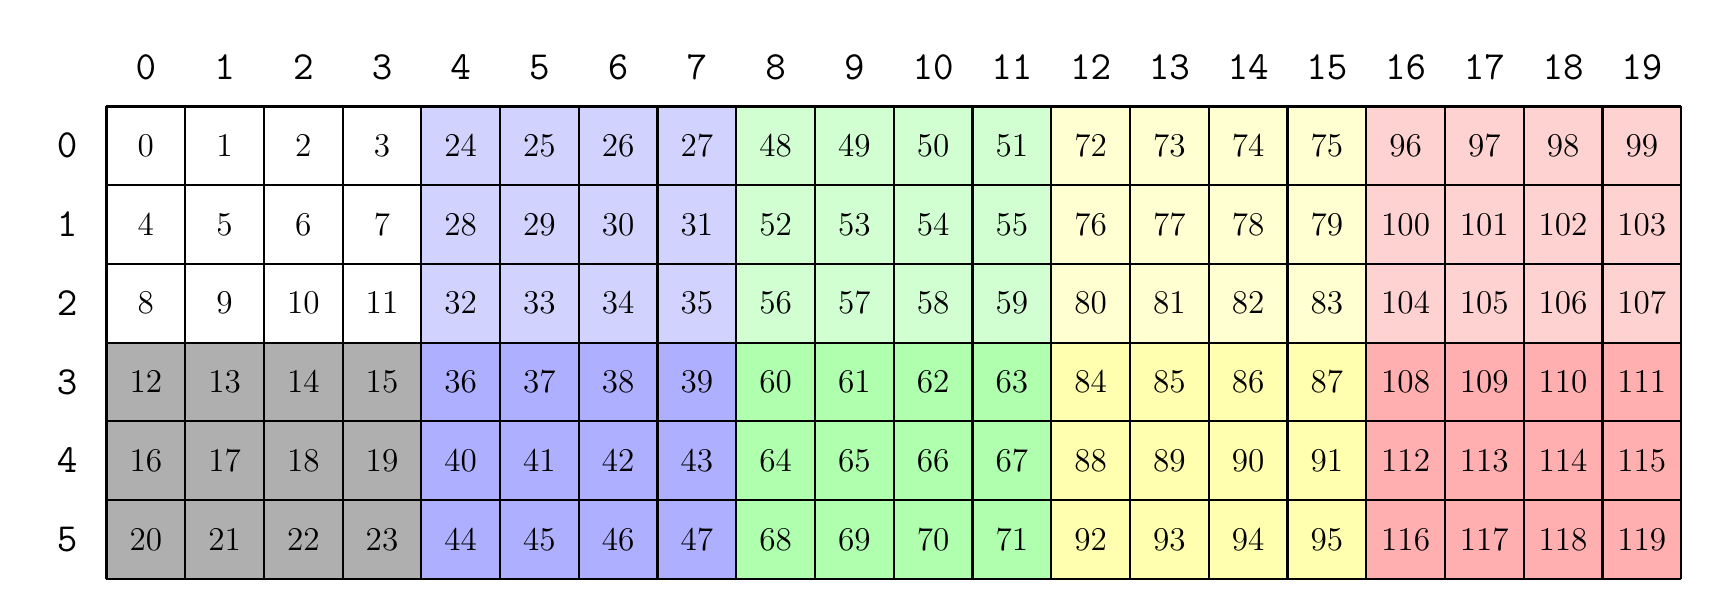
\begin{tikzpicture}[x={(0cm,-1cm)},y={(1cm,0cm)},every node/.style={minimum size=1cm, outer sep=0pt}]
\node[fill={rgb,255:red,255;green,255;blue,255}] at (0,0) {\large 0};
\node[fill={rgb,255:red,255;green,255;blue,255}] at (0,1) {\large 1};
\node[fill={rgb,255:red,255;green,255;blue,255}] at (0,2) {\large 2};
\node[fill={rgb,255:red,255;green,255;blue,255}] at (0,3) {\large 3};
\node[fill={rgb,255:red,210;green,210;blue,255}] at (0,4) {\large 24};
\node[fill={rgb,255:red,210;green,210;blue,255}] at (0,5) {\large 25};
\node[fill={rgb,255:red,210;green,210;blue,255}] at (0,6) {\large 26};
\node[fill={rgb,255:red,210;green,210;blue,255}] at (0,7) {\large 27};
\node[fill={rgb,255:red,210;green,255;blue,210}] at (0,8) {\large 48};
\node[fill={rgb,255:red,210;green,255;blue,210}] at (0,9) {\large 49};
\node[fill={rgb,255:red,210;green,255;blue,210}] at (0,10) {\large 50};
\node[fill={rgb,255:red,210;green,255;blue,210}] at (0,11) {\large 51};
\node[fill={rgb,255:red,255;green,255;blue,210}] at (0,12) {\large 72};
\node[fill={rgb,255:red,255;green,255;blue,210}] at (0,13) {\large 73};
\node[fill={rgb,255:red,255;green,255;blue,210}] at (0,14) {\large 74};
\node[fill={rgb,255:red,255;green,255;blue,210}] at (0,15) {\large 75};
\node[fill={rgb,255:red,255;green,210;blue,210}] at (0,16) {\large 96};
\node[fill={rgb,255:red,255;green,210;blue,210}] at (0,17) {\large 97};
\node[fill={rgb,255:red,255;green,210;blue,210}] at (0,18) {\large 98};
\node[fill={rgb,255:red,255;green,210;blue,210}] at (0,19) {\large 99};
\node[fill={rgb,255:red,255;green,255;blue,255}] at (1,0) {\large 4};
\node[fill={rgb,255:red,255;green,255;blue,255}] at (1,1) {\large 5};
\node[fill={rgb,255:red,255;green,255;blue,255}] at (1,2) {\large 6};
\node[fill={rgb,255:red,255;green,255;blue,255}] at (1,3) {\large 7};
\node[fill={rgb,255:red,210;green,210;blue,255}] at (1,4) {\large 28};
\node[fill={rgb,255:red,210;green,210;blue,255}] at (1,5) {\large 29};
\node[fill={rgb,255:red,210;green,210;blue,255}] at (1,6) {\large 30};
\node[fill={rgb,255:red,210;green,210;blue,255}] at (1,7) {\large 31};
\node[fill={rgb,255:red,210;green,255;blue,210}] at (1,8) {\large 52};
\node[fill={rgb,255:red,210;green,255;blue,210}] at (1,9) {\large 53};
\node[fill={rgb,255:red,210;green,255;blue,210}] at (1,10) {\large 54};
\node[fill={rgb,255:red,210;green,255;blue,210}] at (1,11) {\large 55};
\node[fill={rgb,255:red,255;green,255;blue,210}] at (1,12) {\large 76};
\node[fill={rgb,255:red,255;green,255;blue,210}] at (1,13) {\large 77};
\node[fill={rgb,255:red,255;green,255;blue,210}] at (1,14) {\large 78};
\node[fill={rgb,255:red,255;green,255;blue,210}] at (1,15) {\large 79};
\node[fill={rgb,255:red,255;green,210;blue,210}] at (1,16) {\large 100};
\node[fill={rgb,255:red,255;green,210;blue,210}] at (1,17) {\large 101};
\node[fill={rgb,255:red,255;green,210;blue,210}] at (1,18) {\large 102};
\node[fill={rgb,255:red,255;green,210;blue,210}] at (1,19) {\large 103};
\node[fill={rgb,255:red,255;green,255;blue,255}] at (2,0) {\large 8};
\node[fill={rgb,255:red,255;green,255;blue,255}] at (2,1) {\large 9};
\node[fill={rgb,255:red,255;green,255;blue,255}] at (2,2) {\large 10};
\node[fill={rgb,255:red,255;green,255;blue,255}] at (2,3) {\large 11};
\node[fill={rgb,255:red,210;green,210;blue,255}] at (2,4) {\large 32};
\node[fill={rgb,255:red,210;green,210;blue,255}] at (2,5) {\large 33};
\node[fill={rgb,255:red,210;green,210;blue,255}] at (2,6) {\large 34};
\node[fill={rgb,255:red,210;green,210;blue,255}] at (2,7) {\large 35};
\node[fill={rgb,255:red,210;green,255;blue,210}] at (2,8) {\large 56};
\node[fill={rgb,255:red,210;green,255;blue,210}] at (2,9) {\large 57};
\node[fill={rgb,255:red,210;green,255;blue,210}] at (2,10) {\large 58};
\node[fill={rgb,255:red,210;green,255;blue,210}] at (2,11) {\large 59};
\node[fill={rgb,255:red,255;green,255;blue,210}] at (2,12) {\large 80};
\node[fill={rgb,255:red,255;green,255;blue,210}] at (2,13) {\large 81};
\node[fill={rgb,255:red,255;green,255;blue,210}] at (2,14) {\large 82};
\node[fill={rgb,255:red,255;green,255;blue,210}] at (2,15) {\large 83};
\node[fill={rgb,255:red,255;green,210;blue,210}] at (2,16) {\large 104};
\node[fill={rgb,255:red,255;green,210;blue,210}] at (2,17) {\large 105};
\node[fill={rgb,255:red,255;green,210;blue,210}] at (2,18) {\large 106};
\node[fill={rgb,255:red,255;green,210;blue,210}] at (2,19) {\large 107};
\node[fill={rgb,255:red,175;green,175;blue,175}] at (3,0) {\large 12};
\node[fill={rgb,255:red,175;green,175;blue,175}] at (3,1) {\large 13};
\node[fill={rgb,255:red,175;green,175;blue,175}] at (3,2) {\large 14};
\node[fill={rgb,255:red,175;green,175;blue,175}] at (3,3) {\large 15};
\node[fill={rgb,255:red,175;green,175;blue,255}] at (3,4) {\large 36};
\node[fill={rgb,255:red,175;green,175;blue,255}] at (3,5) {\large 37};
\node[fill={rgb,255:red,175;green,175;blue,255}] at (3,6) {\large 38};
\node[fill={rgb,255:red,175;green,175;blue,255}] at (3,7) {\large 39};
\node[fill={rgb,255:red,175;green,255;blue,175}] at (3,8) {\large 60};
\node[fill={rgb,255:red,175;green,255;blue,175}] at (3,9) {\large 61};
\node[fill={rgb,255:red,175;green,255;blue,175}] at (3,10) {\large 62};
\node[fill={rgb,255:red,175;green,255;blue,175}] at (3,11) {\large 63};
\node[fill={rgb,255:red,255;green,255;blue,175}] at (3,12) {\large 84};
\node[fill={rgb,255:red,255;green,255;blue,175}] at (3,13) {\large 85};
\node[fill={rgb,255:red,255;green,255;blue,175}] at (3,14) {\large 86};
\node[fill={rgb,255:red,255;green,255;blue,175}] at (3,15) {\large 87};
\node[fill={rgb,255:red,255;green,175;blue,175}] at (3,16) {\large 108};
\node[fill={rgb,255:red,255;green,175;blue,175}] at (3,17) {\large 109};
\node[fill={rgb,255:red,255;green,175;blue,175}] at (3,18) {\large 110};
\node[fill={rgb,255:red,255;green,175;blue,175}] at (3,19) {\large 111};
\node[fill={rgb,255:red,175;green,175;blue,175}] at (4,0) {\large 16};
\node[fill={rgb,255:red,175;green,175;blue,175}] at (4,1) {\large 17};
\node[fill={rgb,255:red,175;green,175;blue,175}] at (4,2) {\large 18};
\node[fill={rgb,255:red,175;green,175;blue,175}] at (4,3) {\large 19};
\node[fill={rgb,255:red,175;green,175;blue,255}] at (4,4) {\large 40};
\node[fill={rgb,255:red,175;green,175;blue,255}] at (4,5) {\large 41};
\node[fill={rgb,255:red,175;green,175;blue,255}] at (4,6) {\large 42};
\node[fill={rgb,255:red,175;green,175;blue,255}] at (4,7) {\large 43};
\node[fill={rgb,255:red,175;green,255;blue,175}] at (4,8) {\large 64};
\node[fill={rgb,255:red,175;green,255;blue,175}] at (4,9) {\large 65};
\node[fill={rgb,255:red,175;green,255;blue,175}] at (4,10) {\large 66};
\node[fill={rgb,255:red,175;green,255;blue,175}] at (4,11) {\large 67};
\node[fill={rgb,255:red,255;green,255;blue,175}] at (4,12) {\large 88};
\node[fill={rgb,255:red,255;green,255;blue,175}] at (4,13) {\large 89};
\node[fill={rgb,255:red,255;green,255;blue,175}] at (4,14) {\large 90};
\node[fill={rgb,255:red,255;green,255;blue,175}] at (4,15) {\large 91};
\node[fill={rgb,255:red,255;green,175;blue,175}] at (4,16) {\large 112};
\node[fill={rgb,255:red,255;green,175;blue,175}] at (4,17) {\large 113};
\node[fill={rgb,255:red,255;green,175;blue,175}] at (4,18) {\large 114};
\node[fill={rgb,255:red,255;green,175;blue,175}] at (4,19) {\large 115};
\node[fill={rgb,255:red,175;green,175;blue,175}] at (5,0) {\large 20};
\node[fill={rgb,255:red,175;green,175;blue,175}] at (5,1) {\large 21};
\node[fill={rgb,255:red,175;green,175;blue,175}] at (5,2) {\large 22};
\node[fill={rgb,255:red,175;green,175;blue,175}] at (5,3) {\large 23};
\node[fill={rgb,255:red,175;green,175;blue,255}] at (5,4) {\large 44};
\node[fill={rgb,255:red,175;green,175;blue,255}] at (5,5) {\large 45};
\node[fill={rgb,255:red,175;green,175;blue,255}] at (5,6) {\large 46};
\node[fill={rgb,255:red,175;green,175;blue,255}] at (5,7) {\large 47};
\node[fill={rgb,255:red,175;green,255;blue,175}] at (5,8) {\large 68};
\node[fill={rgb,255:red,175;green,255;blue,175}] at (5,9) {\large 69};
\node[fill={rgb,255:red,175;green,255;blue,175}] at (5,10) {\large 70};
\node[fill={rgb,255:red,175;green,255;blue,175}] at (5,11) {\large 71};
\node[fill={rgb,255:red,255;green,255;blue,175}] at (5,12) {\large 92};
\node[fill={rgb,255:red,255;green,255;blue,175}] at (5,13) {\large 93};
\node[fill={rgb,255:red,255;green,255;blue,175}] at (5,14) {\large 94};
\node[fill={rgb,255:red,255;green,255;blue,175}] at (5,15) {\large 95};
\node[fill={rgb,255:red,255;green,175;blue,175}] at (5,16) {\large 116};
\node[fill={rgb,255:red,255;green,175;blue,175}] at (5,17) {\large 117};
\node[fill={rgb,255:red,255;green,175;blue,175}] at (5,18) {\large 118};
\node[fill={rgb,255:red,255;green,175;blue,175}] at (5,19) {\large 119};
\draw[color=black,thick,shift={(-0.5,-0.5)}] (0,0) grid (6,20);

\node at (0,-1) {\Large{\texttt{0}}};
\node at (1,-1) {\Large{\texttt{1}}};
\node at (2,-1) {\Large{\texttt{2}}};
\node at (3,-1) {\Large{\texttt{3}}};
\node at (4,-1) {\Large{\texttt{4}}};
\node at (5,-1) {\Large{\texttt{5}}};
\node at (-1,0) {\Large{\texttt{0}}};
\node at (-1,1) {\Large{\texttt{1}}};
\node at (-1,2) {\Large{\texttt{2}}};
\node at (-1,3) {\Large{\texttt{3}}};
\node at (-1,4) {\Large{\texttt{4}}};
\node at (-1,5) {\Large{\texttt{5}}};
\node at (-1,6) {\Large{\texttt{6}}};
\node at (-1,7) {\Large{\texttt{7}}};
\node at (-1,8) {\Large{\texttt{8}}};
\node at (-1,9) {\Large{\texttt{9}}};
\node at (-1,10) {\Large{\texttt{10}}};
\node at (-1,11) {\Large{\texttt{11}}};
\node at (-1,12) {\Large{\texttt{12}}};
\node at (-1,13) {\Large{\texttt{13}}};
\node at (-1,14) {\Large{\texttt{14}}};
\node at (-1,15) {\Large{\texttt{15}}};
\node at (-1,16) {\Large{\texttt{16}}};
\node at (-1,17) {\Large{\texttt{17}}};
\node at (-1,18) {\Large{\texttt{18}}};
\node at (-1,19) {\Large{\texttt{19}}};
\end{tikzpicture}
}
\caption{行主序 $(3,4):(4,1)$ 瓦片与列主序 $(2,5):(1,2)$ 铺瓦的 {\tt blocked\_product}。}
\label{fig:blockedproduct}
\end{figure}

操作 {\tt raked\_product} 与分块乘积类似，只是各模以相反的顺序拉链（zip）组合：
\begin{align*}
\begin{array}{cccc}((\textcolor{red}{3}, & \textcolor{red}{4}), & (\textcolor{blue}{2}, & \textcolor{blue}{5})) \\ ((\textcolor{red}{4}, & \textcolor{red}{1}), & (\textcolor{blue}{12}, & \textcolor{blue}{24})) \end{array}
\ \Longrightarrow \
\begin{array}{cccc}((\textcolor{blue}{2}, & \textcolor{red}{3}), & (\textcolor{blue}{5}, & \textcolor{red}{4})) \\ ((\textcolor{blue}{12}, & \textcolor{red}{4}), & (\textcolor{blue}{24}, & \textcolor{red}{1})) \end{array}
\end{align*}
其效果是 $3 {\times} 4$ 瓦片被“耙”（raked）在 $2 {\times} 5$ 瓦片之上，而非“分块”排布。图~\ref{fig:rakedproduct} 画出了得到的布局，其中每个 $3 {\times} 4$ 瓦片都施以底纹。

\begin{figure}[ht]
\centering
%\includegraphics[scale=0.5]{raked_product}
\scalebox{0.5}{
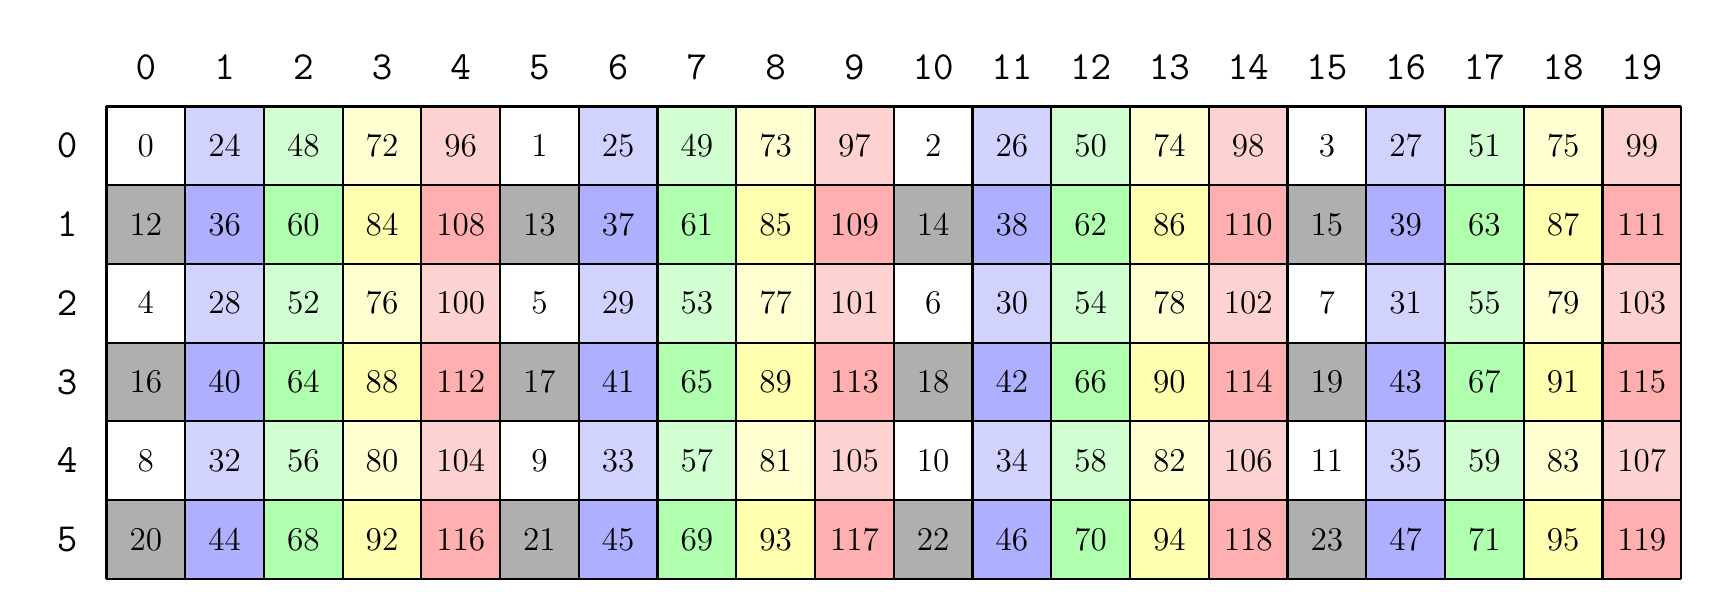
\begin{tikzpicture}[x={(0cm,-1cm)},y={(1cm,0cm)},every node/.style={minimum size=1cm, outer sep=0pt}]

\node[fill={rgb,255:red,255;green,255;blue,255}] at (0,0) {\large 0};
\node[fill={rgb,255:red,210;green,210;blue,255}] at (0,1) {\large 24};
\node[fill={rgb,255:red,210;green,255;blue,210}] at (0,2) {\large 48};
\node[fill={rgb,255:red,255;green,255;blue,210}] at (0,3) {\large 72};
\node[fill={rgb,255:red,255;green,210;blue,210}] at (0,4) {\large 96};
\node[fill={rgb,255:red,255;green,255;blue,255}] at (0,5) {\large 1};
\node[fill={rgb,255:red,210;green,210;blue,255}] at (0,6) {\large 25};
\node[fill={rgb,255:red,210;green,255;blue,210}] at (0,7) {\large 49};
\node[fill={rgb,255:red,255;green,255;blue,210}] at (0,8) {\large 73};
\node[fill={rgb,255:red,255;green,210;blue,210}] at (0,9) {\large 97};
\node[fill={rgb,255:red,255;green,255;blue,255}] at (0,10) {\large 2};
\node[fill={rgb,255:red,210;green,210;blue,255}] at (0,11) {\large 26};
\node[fill={rgb,255:red,210;green,255;blue,210}] at (0,12) {\large 50};
\node[fill={rgb,255:red,255;green,255;blue,210}] at (0,13) {\large 74};
\node[fill={rgb,255:red,255;green,210;blue,210}] at (0,14) {\large 98};
\node[fill={rgb,255:red,255;green,255;blue,255}] at (0,15) {\large 3};
\node[fill={rgb,255:red,210;green,210;blue,255}] at (0,16) {\large 27};
\node[fill={rgb,255:red,210;green,255;blue,210}] at (0,17) {\large 51};
\node[fill={rgb,255:red,255;green,255;blue,210}] at (0,18) {\large 75};
\node[fill={rgb,255:red,255;green,210;blue,210}] at (0,19) {\large 99};
\node[fill={rgb,255:red,175;green,175;blue,175}] at (1,0) {\large 12};
\node[fill={rgb,255:red,175;green,175;blue,255}] at (1,1) {\large 36};
\node[fill={rgb,255:red,175;green,255;blue,175}] at (1,2) {\large 60};
\node[fill={rgb,255:red,255;green,255;blue,175}] at (1,3) {\large 84};
\node[fill={rgb,255:red,255;green,175;blue,175}] at (1,4) {\large 108};
\node[fill={rgb,255:red,175;green,175;blue,175}] at (1,5) {\large 13};
\node[fill={rgb,255:red,175;green,175;blue,255}] at (1,6) {\large 37};
\node[fill={rgb,255:red,175;green,255;blue,175}] at (1,7) {\large 61};
\node[fill={rgb,255:red,255;green,255;blue,175}] at (1,8) {\large 85};
\node[fill={rgb,255:red,255;green,175;blue,175}] at (1,9) {\large 109};
\node[fill={rgb,255:red,175;green,175;blue,175}] at (1,10) {\large 14};
\node[fill={rgb,255:red,175;green,175;blue,255}] at (1,11) {\large 38};
\node[fill={rgb,255:red,175;green,255;blue,175}] at (1,12) {\large 62};
\node[fill={rgb,255:red,255;green,255;blue,175}] at (1,13) {\large 86};
\node[fill={rgb,255:red,255;green,175;blue,175}] at (1,14) {\large 110};
\node[fill={rgb,255:red,175;green,175;blue,175}] at (1,15) {\large 15};
\node[fill={rgb,255:red,175;green,175;blue,255}] at (1,16) {\large 39};
\node[fill={rgb,255:red,175;green,255;blue,175}] at (1,17) {\large 63};
\node[fill={rgb,255:red,255;green,255;blue,175}] at (1,18) {\large 87};
\node[fill={rgb,255:red,255;green,175;blue,175}] at (1,19) {\large 111};
\node[fill={rgb,255:red,255;green,255;blue,255}] at (2,0) {\large 4};
\node[fill={rgb,255:red,210;green,210;blue,255}] at (2,1) {\large 28};
\node[fill={rgb,255:red,210;green,255;blue,210}] at (2,2) {\large 52};
\node[fill={rgb,255:red,255;green,255;blue,210}] at (2,3) {\large 76};
\node[fill={rgb,255:red,255;green,210;blue,210}] at (2,4) {\large 100};
\node[fill={rgb,255:red,255;green,255;blue,255}] at (2,5) {\large 5};
\node[fill={rgb,255:red,210;green,210;blue,255}] at (2,6) {\large 29};
\node[fill={rgb,255:red,210;green,255;blue,210}] at (2,7) {\large 53};
\node[fill={rgb,255:red,255;green,255;blue,210}] at (2,8) {\large 77};
\node[fill={rgb,255:red,255;green,210;blue,210}] at (2,9) {\large 101};
\node[fill={rgb,255:red,255;green,255;blue,255}] at (2,10) {\large 6};
\node[fill={rgb,255:red,210;green,210;blue,255}] at (2,11) {\large 30};
\node[fill={rgb,255:red,210;green,255;blue,210}] at (2,12) {\large 54};
\node[fill={rgb,255:red,255;green,255;blue,210}] at (2,13) {\large 78};
\node[fill={rgb,255:red,255;green,210;blue,210}] at (2,14) {\large 102};
\node[fill={rgb,255:red,255;green,255;blue,255}] at (2,15) {\large 7};
\node[fill={rgb,255:red,210;green,210;blue,255}] at (2,16) {\large 31};
\node[fill={rgb,255:red,210;green,255;blue,210}] at (2,17) {\large 55};
\node[fill={rgb,255:red,255;green,255;blue,210}] at (2,18) {\large 79};
\node[fill={rgb,255:red,255;green,210;blue,210}] at (2,19) {\large 103};
\node[fill={rgb,255:red,175;green,175;blue,175}] at (3,0) {\large 16};
\node[fill={rgb,255:red,175;green,175;blue,255}] at (3,1) {\large 40};
\node[fill={rgb,255:red,175;green,255;blue,175}] at (3,2) {\large 64};
\node[fill={rgb,255:red,255;green,255;blue,175}] at (3,3) {\large 88};
\node[fill={rgb,255:red,255;green,175;blue,175}] at (3,4) {\large 112};
\node[fill={rgb,255:red,175;green,175;blue,175}] at (3,5) {\large 17};
\node[fill={rgb,255:red,175;green,175;blue,255}] at (3,6) {\large 41};
\node[fill={rgb,255:red,175;green,255;blue,175}] at (3,7) {\large 65};
\node[fill={rgb,255:red,255;green,255;blue,175}] at (3,8) {\large 89};
\node[fill={rgb,255:red,255;green,175;blue,175}] at (3,9) {\large 113};
\node[fill={rgb,255:red,175;green,175;blue,175}] at (3,10) {\large 18};
\node[fill={rgb,255:red,175;green,175;blue,255}] at (3,11) {\large 42};
\node[fill={rgb,255:red,175;green,255;blue,175}] at (3,12) {\large 66};
\node[fill={rgb,255:red,255;green,255;blue,175}] at (3,13) {\large 90};
\node[fill={rgb,255:red,255;green,175;blue,175}] at (3,14) {\large 114};
\node[fill={rgb,255:red,175;green,175;blue,175}] at (3,15) {\large 19};
\node[fill={rgb,255:red,175;green,175;blue,255}] at (3,16) {\large 43};
\node[fill={rgb,255:red,175;green,255;blue,175}] at (3,17) {\large 67};
\node[fill={rgb,255:red,255;green,255;blue,175}] at (3,18) {\large 91};
\node[fill={rgb,255:red,255;green,175;blue,175}] at (3,19) {\large 115};
\node[fill={rgb,255:red,255;green,255;blue,255}] at (4,0) {\large 8};
\node[fill={rgb,255:red,210;green,210;blue,255}] at (4,1) {\large 32};
\node[fill={rgb,255:red,210;green,255;blue,210}] at (4,2) {\large 56};
\node[fill={rgb,255:red,255;green,255;blue,210}] at (4,3) {\large 80};
\node[fill={rgb,255:red,255;green,210;blue,210}] at (4,4) {\large 104};
\node[fill={rgb,255:red,255;green,255;blue,255}] at (4,5) {\large 9};
\node[fill={rgb,255:red,210;green,210;blue,255}] at (4,6) {\large 33};
\node[fill={rgb,255:red,210;green,255;blue,210}] at (4,7) {\large 57};
\node[fill={rgb,255:red,255;green,255;blue,210}] at (4,8) {\large 81};
\node[fill={rgb,255:red,255;green,210;blue,210}] at (4,9) {\large 105};
\node[fill={rgb,255:red,255;green,255;blue,255}] at (4,10) {\large 10};
\node[fill={rgb,255:red,210;green,210;blue,255}] at (4,11) {\large 34};
\node[fill={rgb,255:red,210;green,255;blue,210}] at (4,12) {\large 58};
\node[fill={rgb,255:red,255;green,255;blue,210}] at (4,13) {\large 82};
\node[fill={rgb,255:red,255;green,210;blue,210}] at (4,14) {\large 106};
\node[fill={rgb,255:red,255;green,255;blue,255}] at (4,15) {\large 11};
\node[fill={rgb,255:red,210;green,210;blue,255}] at (4,16) {\large 35};
\node[fill={rgb,255:red,210;green,255;blue,210}] at (4,17) {\large 59};
\node[fill={rgb,255:red,255;green,255;blue,210}] at (4,18) {\large 83};
\node[fill={rgb,255:red,255;green,210;blue,210}] at (4,19) {\large 107};
\node[fill={rgb,255:red,175;green,175;blue,175}] at (5,0) {\large 20};
\node[fill={rgb,255:red,175;green,175;blue,255}] at (5,1) {\large 44};
\node[fill={rgb,255:red,175;green,255;blue,175}] at (5,2) {\large 68};
\node[fill={rgb,255:red,255;green,255;blue,175}] at (5,3) {\large 92};
\node[fill={rgb,255:red,255;green,175;blue,175}] at (5,4) {\large 116};
\node[fill={rgb,255:red,175;green,175;blue,175}] at (5,5) {\large 21};
\node[fill={rgb,255:red,175;green,175;blue,255}] at (5,6) {\large 45};
\node[fill={rgb,255:red,175;green,255;blue,175}] at (5,7) {\large 69};
\node[fill={rgb,255:red,255;green,255;blue,175}] at (5,8) {\large 93};
\node[fill={rgb,255:red,255;green,175;blue,175}] at (5,9) {\large 117};
\node[fill={rgb,255:red,175;green,175;blue,175}] at (5,10) {\large 22};
\node[fill={rgb,255:red,175;green,175;blue,255}] at (5,11) {\large 46};
\node[fill={rgb,255:red,175;green,255;blue,175}] at (5,12) {\large 70};
\node[fill={rgb,255:red,255;green,255;blue,175}] at (5,13) {\large 94};
\node[fill={rgb,255:red,255;green,175;blue,175}] at (5,14) {\large 118};
\node[fill={rgb,255:red,175;green,175;blue,175}] at (5,15) {\large 23};
\node[fill={rgb,255:red,175;green,175;blue,255}] at (5,16) {\large 47};
\node[fill={rgb,255:red,175;green,255;blue,175}] at (5,17) {\large 71};
\node[fill={rgb,255:red,255;green,255;blue,175}] at (5,18) {\large 95};
\node[fill={rgb,255:red,255;green,175;blue,175}] at (5,19) {\large 119};
\draw[color=black,thick,shift={(-0.5,-0.5)}] (0,0) grid (6,20);

\node at (0,-1) {\Large{\texttt{0}}};
\node at (1,-1) {\Large{\texttt{1}}};
\node at (2,-1) {\Large{\texttt{2}}};
\node at (3,-1) {\Large{\texttt{3}}};
\node at (4,-1) {\Large{\texttt{4}}};
\node at (5,-1) {\Large{\texttt{5}}};
\node at (-1,0) {\Large{\texttt{0}}};
\node at (-1,1) {\Large{\texttt{1}}};
\node at (-1,2) {\Large{\texttt{2}}};
\node at (-1,3) {\Large{\texttt{3}}};
\node at (-1,4) {\Large{\texttt{4}}};
\node at (-1,5) {\Large{\texttt{5}}};
\node at (-1,6) {\Large{\texttt{6}}};
\node at (-1,7) {\Large{\texttt{7}}};
\node at (-1,8) {\Large{\texttt{8}}};
\node at (-1,9) {\Large{\texttt{9}}};
\node at (-1,10) {\Large{\texttt{10}}};
\node at (-1,11) {\Large{\texttt{11}}};
\node at (-1,12) {\Large{\texttt{12}}};
\node at (-1,13) {\Large{\texttt{13}}};
\node at (-1,14) {\Large{\texttt{14}}};
\node at (-1,15) {\Large{\texttt{15}}};
\node at (-1,16) {\Large{\texttt{16}}};
\node at (-1,17) {\Large{\texttt{17}}};
\node at (-1,18) {\Large{\texttt{18}}};
\node at (-1,19) {\Large{\texttt{19}}};
\end{tikzpicture}
}
\caption{行主序 $(3,4):(4,1)$ 瓦片与列主序 $(2,5):(1,2)$ 铺瓦的 {\tt raked\_product}。}
\label{fig:rakedproduct}
\end{figure}

%The operation {\tt tiled\_product} is another convenience function that simply flattens by one level the second mode of a logical product.

还可以构造逻辑乘积的许多其它版本，它们额外地对模进行分组与重排，以得到方便使用的结果。

\wpssh{应用：逻辑切分}
\label{sec:logical_divide}

两个布局 $\v{A}$ 与 $\v{B}$ 的逻辑切分是一个布局 $\v{R}$，其中“布局 $\v{A}$ 被一分为二：被 $\v{B}$ 指向的元素与未被 $\v{B}$ 指向的元素”。

具体地，我们将逻辑切分定义为一个从两个布局产生一个 2 阶布局的函数
\begin{align*}
\v{A} \oslash \v{B} = \v{A} \circ (\v{B}, \v{B}^*_{\abs{\v{A}}}) = \v{A} \circ \v{B}^\bigstar
\end{align*}
其中 $\v{B}^*_{\abs{\v{A}}}$ 是 $\v{B}$ 相对于布局 $\v{A}$ 的尺寸所取的补。由于该操作意在保留 $\v{A}$ 的全部元素、只是把布局 $\v{A}$ 一分为二，我们要求 $\v{B}^\bigstar = (\v{B},\v{B}^*_{\abs{\v{A}}})$ 满射到 $\Z_{\abs{A}}$。这通常涉及对 $\v{B}^*$ 尺寸的扩展，使得 $\abs{\v{B}^\bigstar} \geq \abs{\v{A}}$。此外，我们要求补 $\v{B}^*$ 在如下意义上“补全”布局 $\v{B}$：$\v{B}^\bigstar = (\v{B},\v{B}^*_{\abs{A}})$ 具有自反广义逆 $\v{B}^+$，满足
\begin{align}
\v{B}^\bigstar \v{B}^+ \v{B}^\bigstar = \v{B}^\bigstar \\
\v{B}^+ \v{B}^\bigstar \v{B}^+ = \v{B}^+
\end{align}

与逻辑乘积操作类似，结果布局 $\v{A} \circ \v{B}$ 的第一个模通常被称为“瓦片”，它在“网格”（即“铺瓦”）布局 $\v{A} \circ \v{B}^*_{\abs{\v{A}}}$ 上被重复。参数 $\v{B}$ 被称为“铺瓦器”，它可以被扩展为不仅仅是布局，如第~\ref{sec:tiler}~节所述。

作为一个直接的例子，常见的需求是从另一个布局中取出某组逻辑元素。例如，要从布局中每隔三个取一个元素，可以使用复合：
\begin{align*}
\begin{array}{c} \textcolor{red}{24} \\ \textcolor{red}{3} \end{array}
\ \circ \
\begin{array}{c} \textcolor{blue}{8} \\ \textcolor{blue}{3} \end{array}
\ &= \
\begin{array}{c} \textcolor{blue}{8} \\ \textcolor{blue}{9} \end{array} \\
\begin{array}{ccc} (\textcolor{red}{6}, & \textcolor{red}{2}, & \textcolor{red}{2}) \\ (\textcolor{red}{2}, & \textcolor{red}{1}, & \textcolor{red}{20}) \end{array}
\ \circ \
\begin{array}{c} \textcolor{blue}{8} \\ \textcolor{blue}{3} \end{array}
\ &= \
\begin{array}{ccc} (\textcolor{blue}{2}, & \textcolor{blue}{2}, & \textcolor{blue}{2}) \\ (\textcolor{blue}{6}, & \textcolor{blue}{1}, & \textcolor{blue}{20}) \end{array}
\end{align*}
在上面两种情形中，都是 24 个元素的布局与布局 $8:3$ 复合，得到每隔三个取一个元素的布局。但左手边布局中“其余”的元素怎么办？逻辑切分把左手边的布局拆成两块：被右手边“命中”的部分与“其余”部分：
\begin{align*}
\begin{array}{c} \textcolor{red}{24} \\ \textcolor{red}{3} \end{array}
\ \oslash \
\begin{array}{c} \textcolor{blue}{8} \\ \textcolor{blue}{3} \end{array}
\ &=& \
\begin{array}{c} \textcolor{red}{24} \\ \textcolor{red}{3} \end{array}
\ \circ \
\begin{array}{cc} (\textcolor{blue}{8}, & 3) \\ (\textcolor{blue}{3}, & 1) \end{array}
\ &=& \
\begin{array}{cc} (\textcolor{blue}{8}, & 3) \\ (\textcolor{blue}{9}, & 3) \end{array} \\
\begin{array}{ccc} (\textcolor{red}{6}, & \textcolor{red}{2}, & \textcolor{red}{2}) \\ (\textcolor{red}{2}, & \textcolor{red}{1}, & \textcolor{red}{20}) \end{array}
\ \oslash \
\begin{array}{c} \textcolor{blue}{8} \\ \textcolor{blue}{3} \end{array}
\ &=& \
\begin{array}{ccc} (\textcolor{red}{6}, & \textcolor{red}{2}, & \textcolor{red}{2}) \\ (\textcolor{red}{2}, & \textcolor{red}{1}, & \textcolor{red}{20}) \end{array}
\ \circ \
\begin{array}{cc} (\textcolor{blue}{8}, & 3) \\ (\textcolor{blue}{3}, & 1) \end{array}
\ &=& \
\begin{array}{cccc} ((\textcolor{blue}{2}, & \textcolor{blue}{2}, & \textcolor{blue}{2}), & 3) \\ ((\textcolor{blue}{6}, & \textcolor{blue}{1}, & \textcolor{blue}{20}), & 2) \end{array}
\end{align*}
其中 $3:1$ 是 $8:3$ 在尺寸 24 之下的补。结果的第一模按要求仍然包含左手边布局中每隔三个取一个的元素，而结果的第二模是这些“瓦片”在原布局中的个数（本例中为 3）以及这些瓦片之间的步幅。补被用来确定缺失了哪些元素、以及以何种顺序保留它们。

\paragraph{相关切分}

与复合类似，人们经常希望按模施加逻辑切分。这里使用同样的记号与策略
\begin{align*}
\v{A} \oslash \langle \v{B},\v{C} \rangle = (\v{A}_0,\v{A}_1) \oslash \langle \v{B},\v{C} \rangle = (\v{A}_0 \oslash \v{B}, \v{A}_1 \oslash \v{C}).
\end{align*}
其直觉在于：能够对列和行独立地执行这些操作，然后视需要重排这些模以构造新布局，这与布局乘积类似。例如，回到第~\ref{sec:tiler}~节中的铺瓦器，将这些铺瓦器用于逻辑切分而非复合，就得到铺瓦器所指向的 $4 {\times} 8$ 子布局组成的 $2 {\times} 2$ 布局。图~\ref{fig:tilers_divide} 展示了这一点，其中可以想象有一个 $2 {\times} 2$ 布局映射到每个单独施以底纹的数据瓦片。

\begin{figure}[ht]
\centering
\begin{subfigure}{0.22\textwidth}
\centering
\resizebox{\linewidth}{!}{
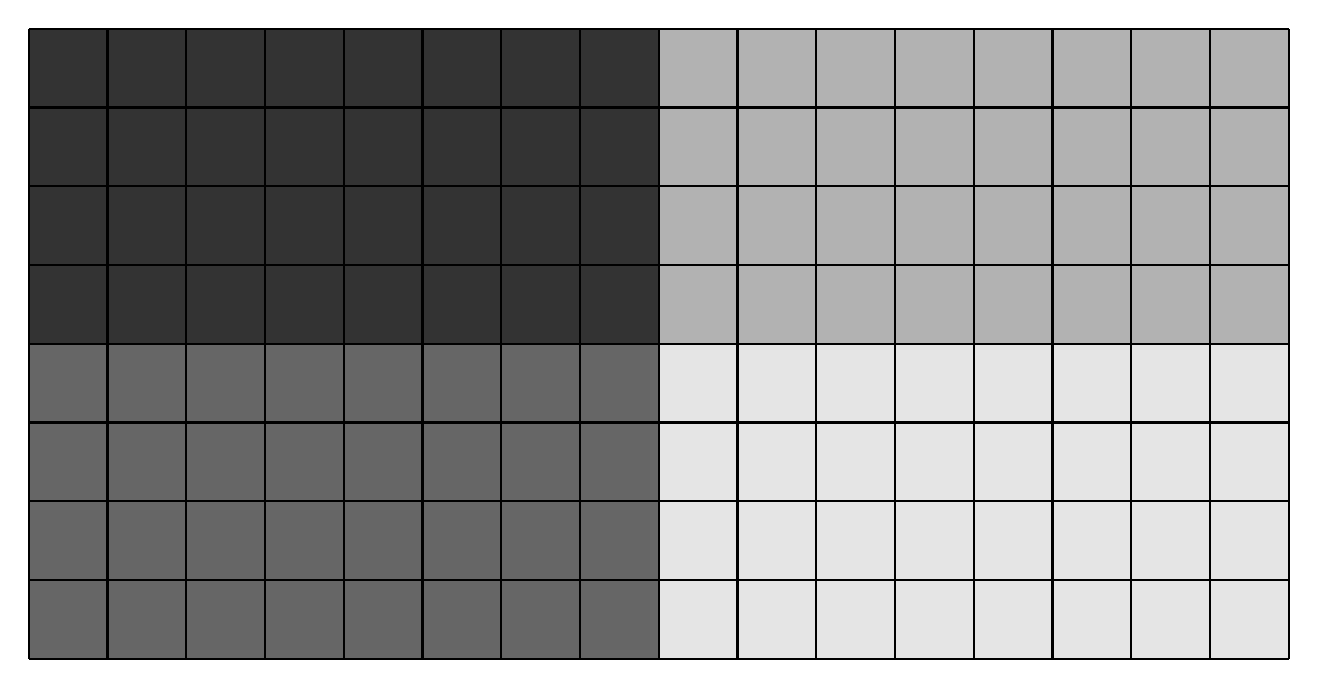
\begin{tikzpicture}[x={(0cm,-1cm)},y={(1cm,0cm)},every node/.style={minimum size=1cm, outer sep=0pt}]
\foreach \i in {0,1,2,3} {
\foreach \j in {0,1,2,3,4,5,6,7} {
\node[fill=black!80!white] at (\i,\j) {};
}}
\foreach \i in {4,5,6,7} {
\foreach \j in {0,1,2,3,4,5,6,7} {
\node[fill=black!60!white] at (\i,\j) {};
}}
\foreach \i in {0,1,2,3} {
\foreach \j in {8,9,10,11,12,13,14,15} {
\node[fill=black!30!white] at (\i,\j) {};
}}
\foreach \i in {4,5,6,7} {
\foreach \j in {8,9,10,11,12,13,14,15} {
\node[fill=black!10!white] at (\i,\j) {};
}}
\draw[color=black,thick,shift={(-0.5,-0.5)}] (0,0) grid (8,16);
\end{tikzpicture}}
\caption{$\langle 4,8 \rangle \equiv \langle 4:1,8:1 \rangle$}
\end{subfigure}\quad
\begin{subfigure}{0.22\textwidth}
\centering
\resizebox{\linewidth}{!}{
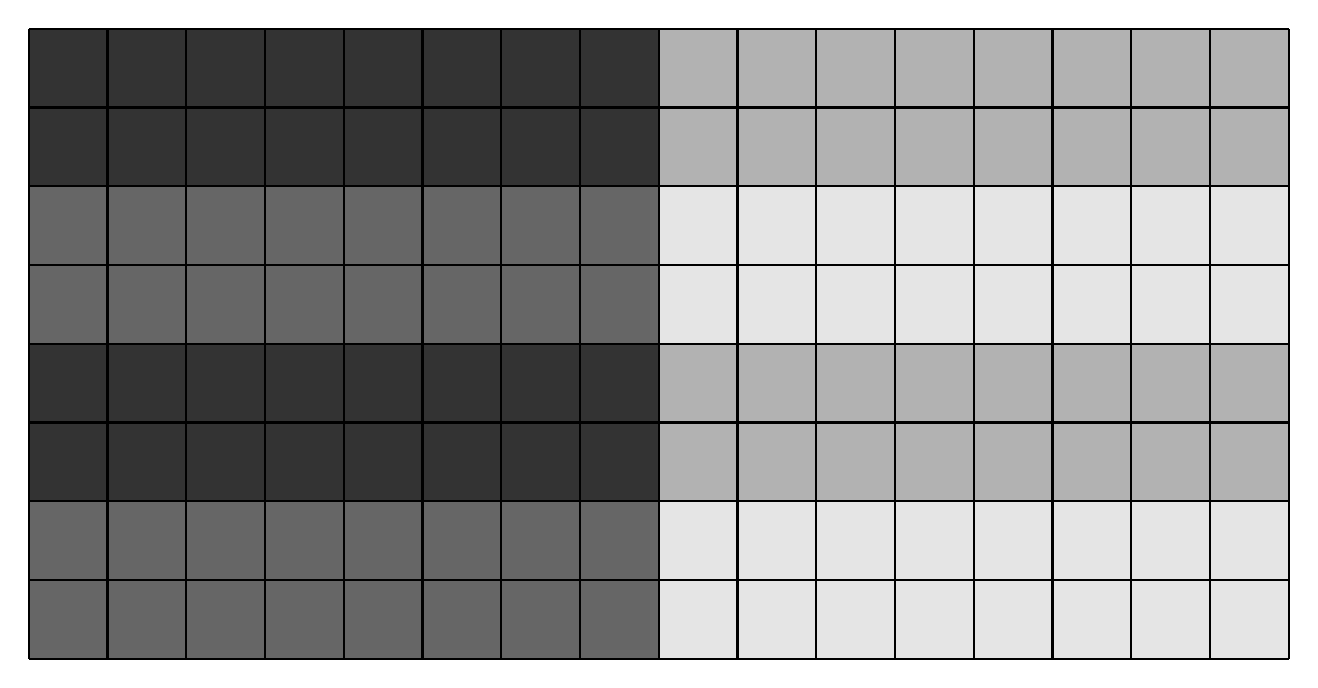
\begin{tikzpicture}[x={(0cm,-1cm)},y={(1cm,0cm)},every node/.style={minimum size=1cm, outer sep=0pt}]
\foreach \i in {0,1,4,5} {
\foreach \j in {0,1,2,3,4,5,6,7} {
\node[fill=black!80!white] at (\i,\j) {};
}}
\foreach \i in {2,3,6,7} {
\foreach \j in {0,1,2,3,4,5,6,7} {
\node[fill=black!60!white] at (\i,\j) {};
}}
\foreach \i in {0,1,4,5} {
\foreach \j in {8,9,10,11,12,13,14,15} {
\node[fill=black!30!white] at (\i,\j) {};
}}
\foreach \i in {2,3,6,7} {
\foreach \j in {8,9,10,11,12,13,14,15} {
\node[fill=black!10!white] at (\i,\j) {};
}}
\draw[color=black,thick,shift={(-0.5,-0.5)}] (0,0) grid (8,16);
\end{tikzpicture}}
\caption{$\langle (2,2):(1,4),8:1 \rangle$}
\end{subfigure}\quad
\begin{subfigure}{0.22\textwidth}
\centering
\resizebox{\linewidth}{!}{
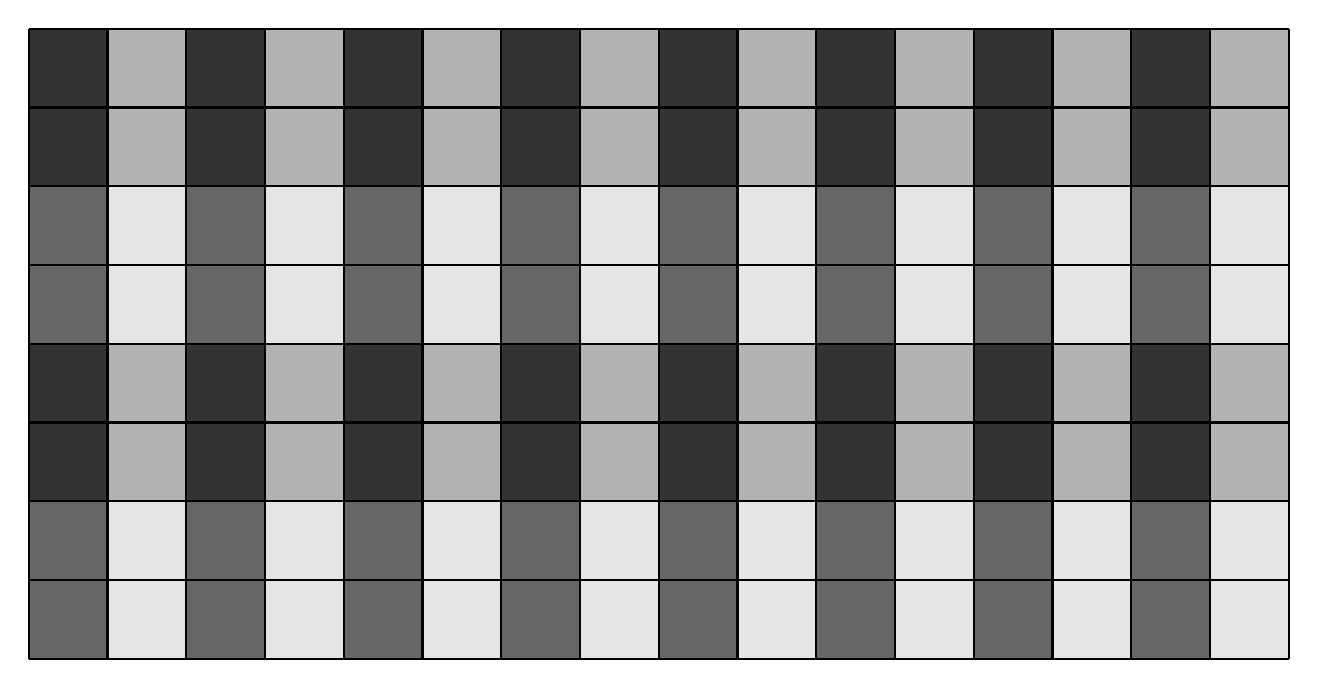
\begin{tikzpicture}[x={(0cm,-1cm)},y={(1cm,0cm)},every node/.style={minimum size=1cm, outer sep=0pt}]
\foreach \i in {0,1,4,5} {
\foreach \j in {0,2,4,6,8,10,12,14} {
\node[fill=black!80!white] at (\i,\j) {};
}}
\foreach \i in {2,3,6,7} {
\foreach \j in {0,2,4,6,8,10,12,14} {
\node[fill=black!60!white] at (\i,\j) {};
}}
\foreach \i in {0,1,4,5} {
\foreach \j in {1,3,5,7,9,11,13,15} {
\node[fill=black!30!white] at (\i,\j) {};
}}
\foreach \i in {2,3,6,7} {
\foreach \j in {1,3,5,7,9,11,13,15} {
\node[fill=black!10!white] at (\i,\j) {};
}}
\draw[color=black,thick,shift={(-0.5,-0.5)}] (0,0) grid (8,16);
\end{tikzpicture}}
\caption{$\langle (2,2):(1,4),8:2 \rangle$}
\end{subfigure}\quad
\begin{subfigure}{0.22\textwidth}
\centering
\resizebox{\linewidth}{!}{
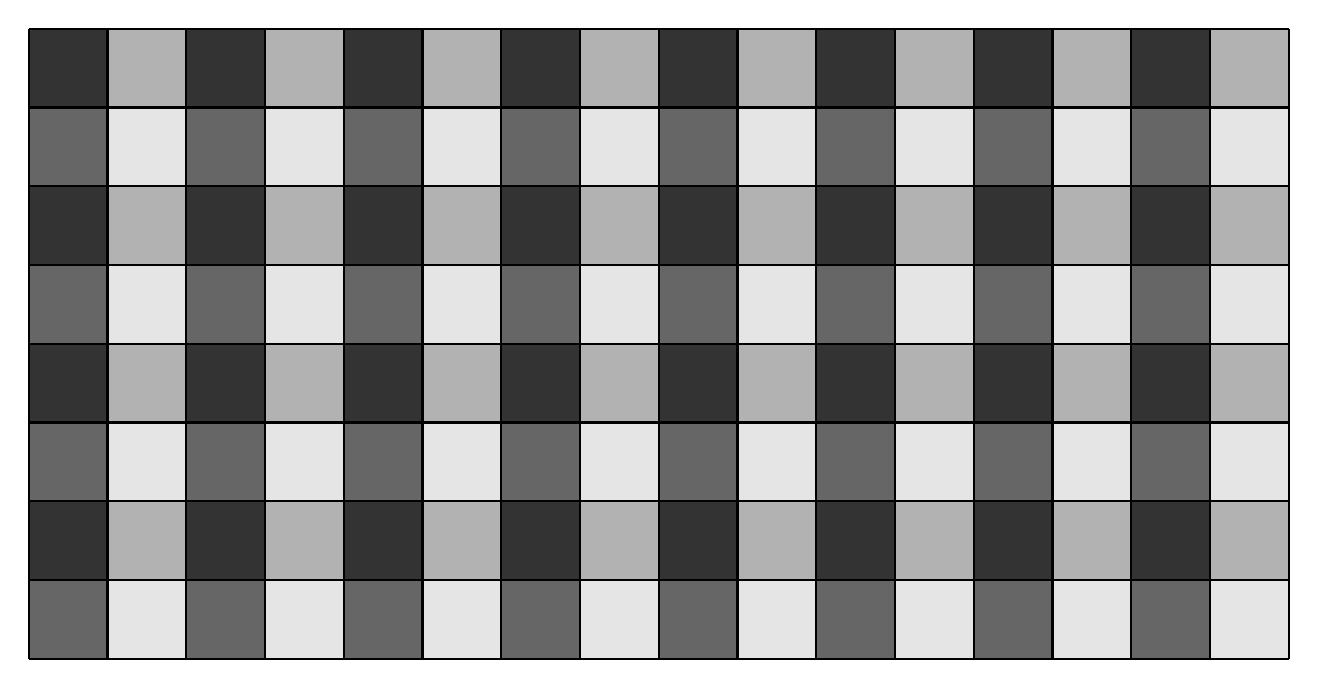
\begin{tikzpicture}[x={(0cm,-1cm)},y={(1cm,0cm)},every node/.style={minimum size=1cm, outer sep=0pt}]
\foreach \i in {0,2,4,6} {
\foreach \j in {0,2,4,6,8,10,12,14} {
\node[fill=black!80!white] at (\i,\j) {};
}}
\foreach \i in {1,3,5,7} {
\foreach \j in {0,2,4,6,8,10,12,14} {
\node[fill=black!60!white] at (\i,\j) {};
}}
\foreach \i in {0,2,4,6} {
\foreach \j in {1,3,5,7,9,11,13,15} {
\node[fill=black!30!white] at (\i,\j) {};
}}
\foreach \i in {1,3,5,7} {
\foreach \j in {1,3,5,7,9,11,13,15} {
\node[fill=black!10!white] at (\i,\j) {};
}}
\draw[color=black,thick,shift={(-0.5,-0.5)}] (0,0) grid (8,16);
\end{tikzpicture}}
\caption{$\langle 4:2,8:2 \rangle$}
\end{subfigure}
\caption{将 $8 {\times} 16$ 布局切分为 $4 {\times} 8$ 瓦片、并以 $2 {\times} 2$ 铺瓦的铺瓦器示例。}
\label{fig:tilers_divide}
\end{figure}

例如，给定布局 $(\textcolor{red}{8},\textcolor{red}{16}):(\textcolor{red}{20},\textcolor{red}{1})$，我们想抽取一个“瓦片”：沿每列向下取 4 个连续元素、沿每行每隔一个取一个元素。按模的逻辑切分给出
\begin{align*}
\begin{array}{cc} (\textcolor{red}{8}, & \textcolor{red}{16})\\
                  (\textcolor{red}{20},& \textcolor{red}{1}) \end{array}
\ \oslash \
\left\langle
\begin{array}{c} \textcolor{blue}{4} \\ \textcolor{blue}{1} \end{array},
\begin{array}{c} \textcolor{blue}{8} \\ \textcolor{blue}{2} \end{array}
\right\rangle
\ = \
\begin{array}{cc} (\textcolor{red}{8}, & \textcolor{red}{16}) \\ (\textcolor{red}{20}, & \textcolor{red}{1}) \end{array}
\ \circ \
\left\langle
\begin{array}{cc} (\textcolor{blue}{4}, & \textcolor{black}{2}) \\ (\textcolor{blue}{1}, & \textcolor{black}{4}) \end{array},
\begin{array}{cc} (\textcolor{blue}{8}, & \textcolor{black}{2}) \\ (\textcolor{blue}{2}, & \textcolor{black}{1}) \end{array}
\right\rangle
\ = \
\begin{array}{cccc}((\textcolor{blue}{4}, & \textcolor{black}{2}), & (\textcolor{blue}{8}, & \textcolor{black}{2})) \\ ((\textcolor{blue}{20}, & \textcolor{black}{80}), & (\textcolor{blue}{2}, & \textcolor{black}{1})) \end{array}
\end{align*}
其中“瓦片”模标为蓝色，“其余”模标为黑色。注意，结果布局仍保持 $8 {\times} 16$，而铺瓦器所指向的元素已被置换到最前面的 $4 {\times} 8$ 块中。

操作 {\tt zipped\_divide} 先执行按模逻辑切分，再把同类模拉链式地组合在一起：
\begin{align*}
\begin{array}{cccc}((\textcolor{blue}{4}, & \textcolor{blue}{8}), & (\textcolor{black}{2}, & \textcolor{black}{2})) \\ ((\textcolor{blue}{20}, & \textcolor{blue}{2}), & (\textcolor{black}{80}, & \textcolor{black}{1})) \end{array}
\end{align*}
这生成了一个“瓦片”模（蓝色），它恰好是铺瓦器所指向的子布局；以及一个“其余”模（黑色），它是遍历各瓦片的子布局。操作 {\tt zipped\_divide} 总是返回一个 2 阶布局结果，其第一模恰好是与铺瓦器的复合，第二模是与补的复合。

软件中一个非常常见的模式是：把数据布局铺瓦成一个瓦片网格，然后为每个处理单元选出特定的瓦片。在 Python 参考实现 PyCuTe（NVIDIA，2026）中，其形式如下：
\begin{python}
data    = Tensor(MyPtr, MyLayoutMxN)   # Tensor：Crd -> Offset
tiler   = (4,8)                        # Tiler：TileCoord -> Crd
data_vt = zipped_divide(data, tiler)   # Compose：(TileCrd,GridCrd) -> Offset
tile    = data_vt[:, blk_id]           # 按一维 block id 切片
tile    = data_vt[:, (blk_x, blk_y)]   # 按二维 block id 切片，二者等价
\end{python}
可以看出，这一模式与第~\ref{sec:layouttv}~节的线程-值分块非常相似，只不过这里真正指定的只有瓦片模，缺失的“网格”模作为铺瓦器的补被计算出来。这个形状为 $(\text{瓦片}, \text{网格})$ 的“补全”铺瓦器随后与数据复合，产生瓦片网格；再在第二模上按块标识符切片，即可为某个处理单元抽取特定的瓦片。

同样可以构造逻辑切分的许多其它版本，它们额外地对模进行分组与重排，以得到方便使用的结果。

\wph{结论}

本文提出了 \CuTe，一个用于表示与操纵张量布局的数学框架，以应对现代 GPU 架构日益增长的复杂性。凭借其分层布局表示，\CuTe 为编写与管理当代硬件上专用张量指令所需的复杂数据布局与分块（partition）模式提供了通用方法。凭借其丰富的代数运算，\CuTe 为高性能线性代数 kernel 开发中布局的操纵与新布局的生成提供了一条有原理依据的途径。二者结合，该表示与代数能够支持复杂的布局与分块、关注点分离，以及静态分析与优化。

\CuTe 布局表示的表达能力已在若干关键应用中被证明极具价值。\CuTe 便于将多种多样的算法——例如广义张量-张量收缩（GETT）与卷积（CONV）——表示为通用矩阵乘法（GEMM）的实例，从而促进代码复用与算法统一性。例如，\CuTe 允许矩阵无论其具体数据布局如何都用 $(m,n)$ 坐标（coordinate）索引，让通用算法与具体布局保持正交；同时，要求特定布局的算法或指令则能够静态地检查、验证并推演它们的张量参数。

\CuTe 布局代数使得张量布局的静态分析与变换成为可能，用以实现并验证通用算法。例如，它可以为 \texttt{COPY} 操作推导最大向量化机会，验证矩阵乘累加（\texttt{MMA}）与 \texttt{COPY} 指令的输入输出布局，并推导出最优的共享内存布局，包括避免 bank 冲突的 swizzle 模式。这些能力把布局管理从易错的手工过程转变为一种系统化、可验证的方法论。为支持对本文定义的学习、实验与验证，纯 Python 参考实现 PyCuTe（NVIDIA，2026）已在 \url{https://github.com/NVlabs/CuTe} 公开发布。

\CuTe 的实际影响体现在它成功部署于生产系统，最显著的是作为 NVIDIA CUTLASS v3 与 v4 库的基础。在 CUTLASS 以及 FlashAttention 等应用中的性能评估表明，\CuTe 的抽象不引入任何性能开销，同时显著加速了软件开发。该框架的采用验证了它的双重承诺：在保持手工优化代码性能特征的同时，大幅降低开发复杂度与开发时间。

展望未来，\CuTe 的数学基础与代数化方法使其成为一个能够持续适应未来架构创新的框架。通过将布局关注点与算法逻辑分离，并提供强大的编译期推理能力，\CuTe 确立了一种面向张量中心编程的方法论，能够满足各类计算系统与应用的需求。

\section*{致谢}
\addcontentsline{toc}{section}{致谢}

作者感谢 Vijay Thakkar 作为 \CuTe 的早期使用者，感谢他在 \CuTe 的普及及其与 CUTLASS 的集成中发挥的关键作用，以及他对 \CuTe 基础设计与部署的重要贡献。他还感谢 Andrew Kerr、Pradeep Ramani 与 Manish Gupta，感谢他们对于在 CUTLASS 中使用 \CuTe 的洞见，以及他们推动 \CuTe 在高性能 kernel 开发中的早期采用。他感谢 Muhammad Osama 与 Duane Merrill 在 \CuTe 原型上的早期实验工作，以及在最初 \CuTe 示例中所做的底层性能优化。最后，作者感谢 Michael Garland、Bastian Hagedorn、Jay Shah 与 Amanda Liu 提出的富有洞见的反馈，以及他们对 \CuTe 规范一次次提出的挑战与质询。


\endgroup
